% volby:
% male × female
% czech × english (zatím funguje jen czech)
% studijní program / obor: api_bc, api_ing, edu_bc, edu_ing
\documentclass[male,czech,api_bc]{kitheses}

% ------------------------
% BALÍČKY PODLE ŠABLONY
% ------------------------
\usepackage{ifthen}

\usepackage{amsmath,amssymb}
\usepackage{graphicx}
\usepackage{color}
\usepackage{array}
\usepackage{longtable}
\usepackage{afterpage}

% Doplňkové balíčky používané v textu práce.
\usepackage{booktabs}
\usepackage{caption}
\usepackage{float}

% workaround for incompatibility of czech babel and biblatex
\iftutex
\else
\usepackage{etoolbox}
\makeatletter
\newcommand\my@hyphen{-}
\newcommand\my@apostroph{'}
\patchcmd\select@language{-}{\my@hyphen}{}{}
\patchcmd\select@language{'}{\my@apostroph}{}{}
\makeatother
\fi

\usepackage{microtype}

\usepackage[style=iso-numeric,shortnumeration=true]{biblatex}
\addbibresource{literature.bib}

% fonty lze měnit (detaily viz šablona ki-thesis.tex)
\iftutex
	\usepackage{fontspec}
	\setmainfont{Libertinus Serif}
	\setsansfont{Libertinus Sans}
	\setmonofont[Scale=MatchLowercase]{Source Code Pro}
	\usepackage{unicode-math}
	\setmathfont{Libertinus Math}
\else
	\usepackage[utf8]{inputenc}
	\usepackage[T1]{fontenc}
	\usepackage{libertinus}
	\renewcommand{\ttdefault}{pxtt}
\fi

\usepackage{csquotes}

% ------------------------
% ÚDAJE O PRÁCI
% ------------------------
\newcommand{\nazevcz}{Vliv modelů AI na určování významných parametrů na RTG snímcích krční páteře}
\newcommand{\nazeven}{Influence of AI Models on Determining Significant Parameters in X-ray Images of the Cervical Spine}
\newcommand{\autor}{Jaroslav Radimský}
\newcommand{\rok}{2026}
\newcommand{\vedouci}{RNDr. Petr Kubera, Ph.D.}
\newcommand{\vedouciDAT}{RNDr. Petru Kuberovi, Ph.D.}

% zvětšuje o 23 % vertikální okraje v tabulkách
\renewcommand{\arraystretch}{1.23}

% nastavení pro záhlaví
\renewcommand{\chaptermark}[1]{\markboth{\arabic{chapter}. #1}{}}
\pagestyle{fancy}

% nastavení odkazů
\usepackage{url}
\usepackage{varioref}
\usepackage[unicode=true,pdfusetitle,
 bookmarks=true,
 breaklinks=false,pdfborder={0 0 1},backref=false,colorlinks=false]{hyperref}

\newcommand{\UV}[1]{\quotedblbase#1\textquotedblleft}

\raggedbottom

%%%%%%%%%%%%%%%%%%%%%%%%%%%%%%%%%%%%%%%%%%%%%%
% vlastní začátek dokumentu podle šablony
%%%%%%%%%%%%%%%%%%%%%%%%%%%%%%%%%%%%%%%%%%%%%%

\begin{document}
\thispagestyle{empty}
\begin{center}
{
\LARGE
\univerzita\\[16pt]
\fakulta
}

\vspace{2cm}
\resizebox{8.42cm}{!}{%
\ifthenelse{\boolean{czech}}
{
\includegraphics{images/LOGO_PRF_CZ_RGB_standard.jpg}}
{\includegraphics{LOGO_PRF_EN_RGB_standard.jpg}}}

\vspace{2cm}
{
\Huge\sffamily
\nazevcz\par
\vspace{0.6cm}
\Large\scshape \ifthenelse{\boolean{bc}}{bakalářská}{diplomová} práce
}
\end{center}

\vfill
{
\large
\begin{tabular}{>{\bfseries}rl}
    Vypracoval:      & \autor\\
    Vedoucí práce:   & \vedouci\\
&\\
Studijní program:    & \program
\end{tabular}
}
\vspace{1.5cm}
\begin{center}
  \Large\scshape Ústí nad Labem \rok
\end{center}

\cleardoublepage
\thispagestyle{empty}
\pagecolor{yellow}
{\Large Namísto žlutých stránek vložte digitálně podepsané zadání kvalifikační práce poskytnuté vedoucím katedry.\\
Zadání musí zaujímat právě dvě strany.
}

Zadání je nutno vložit jako PDF pomocí některého nástroje, který umožňuje editaci dokumentů se zachováním elektronického podpisu.

\clearpage
\thispagestyle{empty}
\afterpage{\nopagecolor}
~
\clearpage

\thispagestyle{empty}
{\bfseries Prohlášení}

\vspace{0.5cm}
Prohlašuji, že jsem tuto \ifthenelse{\boolean{bc}}{bakalářskou}{diplomovou} práci vypracoval\ifthenelse{\boolean{feminum}}{a}{}
samostatně a použil\ifthenelse{\boolean{feminum}}{a}{}
jen pramenů, které cituji a uvádím v přiloženém seznamu literatury.

\vspace{0.5em}

Byl\ifthenelse{\boolean{feminum}}{a}{} jsem seznámen\ifthenelse{\boolean{feminum}}{a}{}
s tím, že se na moji práci vztahují práva a povinnosti vyplývající ze
zákona č.~121/2000 Sb., ve znění zákona č.~81/2005 Sb., autorský zákon, zejména se
skutečností, že Univerzita Jana Evangelisty Purkyně v Ústí nad Labem má právo na uzavření
licenční smlouvy o užití této práce jako školního díla podle § 60 odst. 1 autorského zákona, a
s tím, že pokud dojde k užití této práce mnou nebo bude poskytnuta licence o užití jinému
subjektu, je Univerzita Jana Evangelisty Purkyně v Ústí nad Labem oprávněna ode mne
požadovat přiměřený příspěvek na úhradu nákladu, které na vytvoření díla vynaložila, a to
podle okolností až do jejich skutečné výše.

\vspace{2em}

V Ústí nad Labem dne \today \hfill Podpis: \makebox[4cm][s]{\dotfill}

\cleardoublepage
\thispagestyle{empty}
~
\vfill

\begin{flushright}
    Děkuji vedoucímu práce \vedouciDAT\\
    za cenné rady a pomoc při tvorbě bakalářské práce.
\end{flushright}

\cleardoublepage

\textsc{\nazevcz}

\textbf{Abstrakt:}

Automatická analýza rentgenových (RTG) snímků krční páteře má značný klinický význam, neboť může lékařům pomoci rychleji a objektivněji posoudit úspěšnost obratlové fúze po operaci. Ruční hodnocení těchto snímků je časově náročné a subjektivní, proto roste zájem o metody využívající hluboké učení. Vývoj spolehlivých algoritmů pro automatické rozpoznávání anatomických struktur a klíčových bodů krční páteře představuje důležitý krok směrem k efektivnější a přesnější klinické diagnostice.

Hlavním cílem práce je srovnání dvou přístupů hlubokého učení pro automatickou analýzu RTG snímků krční páteře, které se liší způsobem určování klíčových bodů závislých na poloze jednotlivých obratlů vůči sobě.

\textbf{Klíčová slova:} hluboké učení, medicínské zobrazování, RTG krční páteře, segmentace, detekce klíčových bodů

\bigskip

\textsc{\nazeven}

\textbf{Abstract:}

Automatic analysis of X-ray (radiographic, RTG) images of the cervical spine has significant clinical importance, as it can help physicians assess the success of vertebral fusion after surgery more quickly and objectively. Manual evaluation of these images is time-consuming and subjective; therefore, there is growing interest in methods based on deep learning. The development of reliable algorithms for the automatic recognition of anatomical structures and key points of the cervical spine represents an important step toward more efficient and accurate clinical diagnosis.

The main objective of this thesis is to compare two deep learning approaches for the automatic analysis of cervical spine X-ray images, which differ in the way they determine key points depending on the relative positions of individual vertebrae.

\textbf{Keywords:} deep learning, medical imaging, cervical spine X-ray, segmentation, keypoint detection

\tableofcontents

\addchap{Úvod}

Degenerativní změny, deformity a další patologické stavy krční páteře patří mezi časté problémy klinické praxe, přičemž jejich správné vyhodnocení je zásadní pro stanovení diagnózy, plánování léčby i sledování pooperačního vývoje. V diagnostice těchto stavů hrají významnou roli boční rentgenové (RTG) snímky krční páteře, z nichž lze odvozovat řadu radiologických parametrů popisujících vzájemné postavení obratlů a celkovou sagitální rovnováhu páteře. Mezi často sledované charakteristiky patří například Cobbův úhel C2--C7, sagitální vertikální osa nebo segmentové úhly jednotlivých pohybových segmentů. Přestože jsou tato měření v klinické praxi běžně využívána, jejich manuální stanovování je časově náročné a může být zatíženo určitou mírou subjektivity.

Cílem práce je navrhnout, implementovat a ověřit dva přístupy k automatizovanému určování klíčových bodů na RTG snímcích krční páteře a následnému výpočtu radiologických metrik. Prvním přístupem je segmentace anatomických struktur s následným postprocessingem pro extrakci klíčových bodů. Druhým přístupem je přímá detekce klíčových bodů.

Dílčími cíli práce je implementace a otestování obou přístupů, návrh a optimalizace postprocessingu s cílem zvýšit přesnost detekce klíčových bodů a následné porovnání dosažených výsledků na základě přesnosti určených charakteristik (Cobbova úhlu, Jacksonova úhlu a dalších odvozených metrik). Součástí práce je rovněž zhodnocení obou metod z hlediska přesnosti, spolehlivosti a výpočetní náročnosti a formulace doporučeného postupu pro automatizované hodnocení RTG snímků krční páteře.

Práce je členěna do jedenácti kapitol. V kapitole \textit{Úvod} je vymezen cíl práce, dílčí cíle a motivace řešeného problému. Kapitola \textit{Medicínské zobrazování krční páteře a význam analýzy RTG} shrnuje základní poznatky o zobrazování krční páteře a významu radiologického hodnocení. V kapitole \textit{Popis klíčových charakteristik krční páteře} jsou popsány sledované anatomické a radiologické parametry. Kapitola \textit{Přehled přístupů hlubokého učení v medicínském zobrazování} uvádí teoretický přehled metod hlubokého učení se zaměřením na úlohy segmentace, detekce a lokalizace klíčových bodů.

V kapitole \textit{Použité modely pro segmentaci a detekci klíčových bodů} jsou představeny modely využité v práci, zejména přístupy založené na architekturách typu U-Net a HRNet. Kapitola \textit{Použité knihovny a frameworky} popisuje softwarové nástroje a knihovny použité při implementaci. V kapitole \textit{Extrakce klíčových bodů ze segmentační masky} je popsán navržený postprocessing pro získání klíčových bodů ze segmentačních výstupů. Kapitola \textit{Popis provedených experimentů} se věnuje datasetu, metodice experimentů, trénování modelů a způsobu vyhodnocení. V kapitole \textit{Výsledky} jsou prezentovány a porovnány dosažené výsledky segmentačního a detekčního přístupu. Kapitola \textit{Závěr} shrnuje hlavní přínosy práce, dosažené výsledky a možná omezení navrženého řešení. Poslední kapitola \textit{Externí Přílohy} obsahuje doplňující materiály.


\chapter{Medicínské zobrazování krční páteře a význam analýzy RTG}

Rentgenové (RTG) vyšetření krční páteře představuje jeden ze základních zobrazovacích nástrojů v klinické praxi při diagnostice onemocnění pohybového aparátu a nervového systému. Díky své široké dostupnosti, nízké finanční náročnosti a relativně malé radiační zátěži je RTG často používáno jako první vyšetřovací metoda při podezření na degenerativní změny, traumatická poranění nebo pooperační komplikace v oblasti krční páteře. Zejména laterální projekce \footnote{Laterální projekce označuje rentgenové zobrazení provedené z bočního pohledu, kdy paprsky procházejí tělem z jedné strany na druhou. U krční páteře tento typ projekce umožňuje dobře zobrazit sagitální zakřivení, vzájemné postavení obratlů a meziobratlové prostory.} poskytuje zásadní informace o sagitálním zakřivení páteře, postavení jednotlivých obratlů a výšce meziobratlových prostor, které jsou klíčové pro další klinické rozhodování \cite{Scheer2013}.

Analýza RTG snímků krční páteře se v klinické praxi zaměřuje především na hodnocení sagitální rovnováhy a zakřivení páteře, které mají přímý vliv na biomechaniku krční oblasti a kvalitu života pacienta. Mezi nejčastěji sledované parametry patří Cobbův úhel, Jacksonův úhel nebo sagitální vertikální osa (SVA), jež slouží k posouzení fyziologického či patologického postavení krční páteře. Odchylky od normálního zakřivení mohou vést k chronickým bolestem, omezení hybnosti nebo k neurologickým obtížím, například při kompresi míchy či nervových kořenů \cite{Scheer2013}.

V současné klinické praxi je však hodnocení těchto parametrů založeno převážně na manuální analýze RTG snímků. Lékař nebo radiolog musí na snímku nejprve identifikovat jednotlivé obratle, zpravidla v rozsahu C2–C7, a následně ručně vyznačit referenční body, koncové ploténky nebo osy obratlových těl. Na základě těchto konstrukcí jsou pomocí měřicích nástrojů v PACS systémech nebo specializovaném softwaru dopočítávány úhly a vzdálenosti charakterizující zakřivení krční páteře \cite{Scheer2013}.

Tento manuální postup je nejen časově náročný, ale také značně závislý na zkušenosti hodnotitele. Různí lékaři mohou volit mírně odlišné referenční body nebo interpretační strategie, což vede k variabilitě naměřených hodnot mezi odlišnými lékaři a institucemi. Subjektivita měření může ovlivnit jak samotnou diagnostiku, tak i následné rozhodování o léčebném postupu, zejména u hraničních nebo mírných patologických nálezů \cite{Ran2024}.

Dalším omezením manuální analýzy RTG snímků je její omezená škálovatelnost v prostředí moderní zdravotní péče. S rostoucím počtem pacientů a obrazových dat se ruční měření stává obtížně udržitelným, zejména v kontextu rutinní klinické praxe. Tradiční přístup
vyžadující manuální anotace a výpočty tak představuje významnou zátěž pro zdravotnický personál a může zpomalovat diagnostický proces \cite{Huang2025}.

Uvedené limity vedou k rostoucímu zájmu o automatizované metody analýzy RTG snímků krční páteře, zejména s využitím metod hlubokého učení. Tyto přístupy slibují objektivní, reprodukovatelné a časově efektivní stanovení klinicky významných parametrů, čímž mohou významně přispět ke zlepšení diagnostického workflow a podpořit rozhodování lékaře. Automatizace analýzy RTG snímků tak představuje perspektivní směr dalšího vývoje medicínského zobrazování v oblasti krční páteře \cite{Huang2025}.

Ačkoli je v běžném PACS workflow hodnocení laterálních RTG snímků krční páteře stále převážně manuální, existují již specializované softwarové nástroje, které část analýzy automatizují nebo alespoň významně zjednodušují. Příkladem je platforma Surgimap, kterou výrobce uvádí jako FDA-cleared a HIPAA-compliant a která nabízí sagitální, koronální a cervikální „wizardy“ pro rychlé měření radiografických parametrů páteře; oficiální web současně uvádí používání více než 15\,000 zdravotnickými profesionály \cite{SurgimapOfficial2026,SurgimapFeatures2026}. Klinická studie publikovaná v roce 2023 navíc popisuje použití Surgimapu jako semi-automatického nástroje při porovnání spinopelvických měření mezi radiology a spinálními chirurgy, což potvrzuje jeho praktické nasazení mimo čistě experimentální prostředí \cite{Fleiderman2023}.

Dalším příkladem je ekosystém EOS imaging, zahrnující systémy EOSedge, sterEOS a spineEOS. Podle výrobce je tato platforma využívána ve více než 500 zdravotnických zařízeních po světě a podporuje více než 1 milion vyšetření ročně \cite{EOSOfficial2026}. Oficiální dokumentace současně uvádí, že sterEOS poskytuje interaktivní 2D/3D měřicí nástroje pro muskuloskeletální RTG snímky a že software sterEOS byl již dříve rozšířen o automatický výpočet více než 100 klinických parametrů relevantních pro diagnostiku a chirurgické plánování \cite{EOSImagingSolutions2026,EOSFDA2014}. Novější platforma EOS Insight je výrobcem popisována jako webová AI platforma, která umožňuje automatizovat hodnocení sagitálního vyvážení z vyšetření EOSedge několik minut po provedení snímku \cite{EOSInsight2025}. Je však třeba zdůraznit, že tento workflow je vázán na specializovaný zobrazovací ekosystém EOS a neodpovídá přímo běžné analýze standardních laterálních RTG snímků krční páteře v konvenčním PACS.

Současně platí, že plně automatická analýza přímo z konvenčních laterálních RTG snímků krční páteře je v literatuře dosud popisována převážně na úrovni výzkumných prototypů. Fujita et al. vyvinuli aplikaci pro automatické měření rozsahu pohybu na flexně-extenčních snímcích krční páteře a ukázali přesnost srovnatelnou se spinálními chirurgy \cite{Fujita2022}. Shim et al. následně publikovali systém pro automatickou segmentaci a výpočet diagnostických metrik z krčních RTG snímků, včetně cSVA a cervikální lordózy, a poukázali na jeho potenciál pro diagnostiku poranění a hodnocení pooperačních výsledků \cite{Shim2024}. V dostupných pracích jsou tyto systémy prezentovány především jako výzkumné prototypy.

Z pohledu této práce tedy lze konstatovat, že určité formy automatizace analýzy RTG snímků páteře již v praxi existují, avšak zpravidla mají charakter specializovaných semi-automatických plánovacích nástrojů nebo jsou vázány na dedikované zobrazovací platformy. Plně automatická a široce rozšířená analýza běžných laterálních RTG snímků krční páteře zatím podle dostupných zdrojů nepředstavuje standardní součást rutinní klinické praxe.


\chapter{Popis klíčových charakteristik krční páteře}
\label{sec:metrics}

\begin{figure}[htbp]
\centering
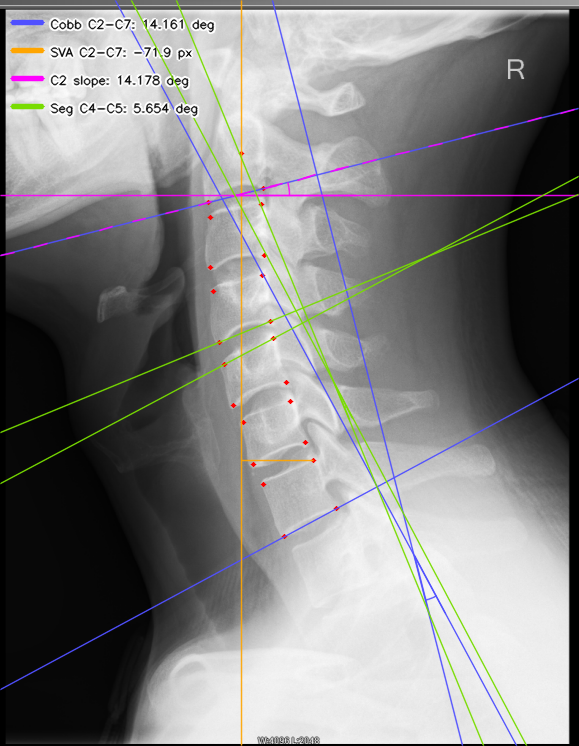
\includegraphics[width=0.82\textwidth]{images/4811033_all_metrics.png}
\caption{Ukázka vybraných klinických metrik vykreslených v jednom snímku. Červeně je znázorněn Cobbův úhel C2--C7, oranžově sagitální osa C2--C7, fialově sklon C2 a zeleně segmentový úhel C4--C5. Obrázek ilustruje způsob konstrukce metrik z lokalizovaných anatomických bodů.}
\label{fig:metrics_visualization}
\end{figure}

Hodnocení sagitálního profilu krční páteře je v klinické praxi založeno na souboru standardizovaných radiologických parametrů, které popisují zakřivení, sklon jednotlivých segmentů a prostorové postavení krční páteře vůči zbytku axiálního skeletu. Tyto metriky jsou běžně stanovovány z laterálních RTG snímků a slouží k posouzení fyziologického či patologického zakřivení krční páteře, k hodnocení degenerativních změn a k analýze pooperačních stavů. Definice jednotlivých charakteristik v této kapitole vycházejí z klinicky používaných měření popsaných v disertační práci MUDr. Martina Bolchy \cite{Bolcha2025}.

\section*{Cobbův úhel C2--C7}

Krční lordóza je nejčastěji kvantifikována pomocí Cobbova úhlu mezi obratli C2 a C7. Tento úhel je klinicky definován jako úhel mezi linií dolní krycí plochy obratle C2 a linií dolní krycí plochy obratle C7 na laterálním RTG snímku. Znaménko úhlu přitom určuje charakter zakřivení, kdy záporné hodnoty odpovídají lordóze a kladné hodnoty kyfotickému zakřivení krční páteře \cite{Bolcha2025}. Konstrukce této metriky je schematicky znázorněna na obr.~\ref{fig:metrics_visualization}, kde je Cobbův úhel vyznačen červeně.

Pro účely automatizované analýzy lze dolní krycí plochy obratlů C2 a C7 popsat pomocí dvojic bodů odpovídajících jejich levému a pravému okraji. Označíme-li tyto body jako $\mathbf{p}_{C2}^{BL}$, $\mathbf{p}_{C2}^{BR}$ a $\mathbf{p}_{C7}^{BL}$, $\mathbf{p}_{C7}^{BR}$, lze směrové vektory jednotlivých krycích ploch definovat vztahem:
\begin{equation}\label{eq:vectors_cobb}
\mathbf{v}_1 = \mathbf{p}_{C2}^{BR} - \mathbf{p}_{C2}^{BL}, \quad
\mathbf{v}_2 = \mathbf{p}_{C7}^{BR} - \mathbf{p}_{C7}^{BL}.
\end{equation}

Samotný Cobbův úhel je následně určen jako úhel mezi těmito vektory.

\section*{Jacksonův úhel C2--C7}

Jacksonův úhel představuje alternativní způsob vyjádření sagitálního zakřivení krční páteře. Klinicky je definován jako úhel mezi linií vedenou podél zadní strany těla obratle C2 a linií vedenou podél zadní strany těla obratle C7 \cite{Bolcha2025}. Na rozdíl od Cobbova úhlu tedy nevychází z krycích ploch, ale z orientace zadních hran obratlových těl.

Označíme-li dva body ležící na zadní hraně obratle C2 jako $\mathbf{p}_{C2}^{P1}$ a $\mathbf{p}_{C2}^{P2}$ a analogicky dva body na zadní hraně obratle C7 jako $\mathbf{p}_{C7}^{P1}$ a $\mathbf{p}_{C7}^{P2}$, lze směrové vektory obou hran zapsat jako:
\begin{equation}
\mathbf{u}_1 = \mathbf{p}_{C2}^{P2} - \mathbf{p}_{C2}^{P1}, \quad
\mathbf{u}_2 = \mathbf{p}_{C7}^{P2} - \mathbf{p}_{C7}^{P1}.
\end{equation}

Jacksonův úhel je pak určen jako úhel mezi těmito vektory:
\begin{equation}
\theta_{Jackson} = \frac{180}{\pi}\,\arctan2(u_{1x}u_{2y} - u_{1y}u_{2x}, \; u_{1x}u_{2x} + u_{1y}u_{2y}).
\end{equation}

\section*{Sagitální vertikální osa C2--C7 (SVA)}

Sagitální vertikální osa C2--C7 (SVA) je vzdálenostní parametr popisující předozadní postavení hlavy a krční páteře. Klinicky je definována jako horizontální vzdálenost mezi vertikální linií spuštěnou ze středu těla obratle C2 ($\mathbf{x}_{C2}^{centroid}$) a zadním horním okrajem těla obratle C7 ($\mathbf{x}_{C7}^{top\ right}$). Tento parametr poskytuje informaci o sagitální rovnováze krční páteře a je významným ukazatelem funkčního zatížení krčního úseku \cite{Bolcha2025}. Konstrukce SVA je znázorněna na obr.~\ref{fig:metrics_visualization} oranžově.

V geometrickém pojetí lze SVA vyjádřit jako rozdíl horizontálních souřadnic příslušných referenčních bodů:
\begin{equation}\label{eq:sva_c2c7}
\mathrm{SVA}_{C2-C7} = {x}_{C2}^{centroid} - {x}_{C7}^{top\ right}.
\end{equation}

\section*{Sklon obratle C2 (C2 slope)}

Sklon obratle C2 je lokální úhlová charakteristika definovaná jako úhel mezi horizontální linií a linií podél dolní krycí plochy obratle C2. Tento parametr popisuje orientaci horní části krční páteře a je významný zejména při hodnocení vztahu mezi lokální a globální sagitální osou krční páteře \cite{Bolcha2025}. Konstrukce této metriky je uvedena na obr.~\ref{fig:metrics_visualization}, kde je sklon C2 znázorněn fialově.

Je-li dolní krycí plocha obratle C2 popsána body $\mathbf{p}_{C2}^{BL}$ a $\mathbf{p}_{C2}^{BR}$, lze sklon obratle vyjádřit pomocí vztahů:
\begin{equation}\label{eq:c2_slope_delta}
\Delta x = x_{BR} - x_{BL}, \quad \Delta y = y_{BR} - y_{BL},
\end{equation}
a výsledný úhel pak vypočítat jako:
\begin{equation}\label{eq:c2_slope_angle}
\varphi_{C2} = \arctan2(\Delta y, \Delta x), \quad
\varphi_{deg} = \frac{180}{\pi}\,\varphi_{C2}.
\end{equation}

\section*{Segmentové úhlové charakteristiky}

Kromě celkového zakřivení krční páteře jsou v klinické praxi sledovány také segmentové úhlové charakteristiky mezi sousedními obratli. Tyto parametry jsou definovány jako úhly mezi sousedními segmenty krční páteře, například C2--C3, C3--C4 až C6--C7. Segmentové úhly umožňují detailní hodnocení lokálních změn zakřivení, které mohou mít klinický význam zejména u degenerativních nebo pooperačních změn \cite{Bolcha2025}. Na obr.~\ref{fig:metrics_visualization} je jako příklad znázorněn segmentový úhel C4--C5 zelenou barvou.

Je-li dolní krycí plocha horního obratle daného segmentu popsána dvojicí bodů $\mathbf{p}_{u}^{BL}$ a $\mathbf{p}_{u}^{BR}$ a horní krycí plocha dolního obratle dvojicí bodů $\mathbf{p}_{l}^{TL}$ a $\mathbf{p}_{l}^{TR}$, lze směrové vektory obou linií vyjádřit jako:
\begin{equation}
\mathbf{s}_1 = \mathbf{p}_{u}^{BR} - \mathbf{p}_{u}^{BL}, \quad
\mathbf{s}_2 = \mathbf{p}_{l}^{TR} - \mathbf{p}_{l}^{TL}.
\end{equation}

Segmentový úhel je pak definován jako úhel mezi těmito vektory:
\begin{equation}
\theta_{seg} = \frac{180}{\pi}\,\arctan2(s_{1x}s_{2y} - s_{1y}s_{2x}, \; s_{1x}s_{2x} + s_{1y}s_{2y}).
\end{equation}

\chapter{Přehled přístupů hlubokého učení v medicínském zobrazování}

Hluboké učení představuje v současnosti jeden z nejvýznamnějších směrů automatizované analýzy medicínských obrazových dat. Jeho hlavní přínos spočívá v tom, že modely dokáží učit reprezentace přímo z dat, bez nutnosti ručně navrhovat příznaky pro každý konkrétní diagnostický problém. Podle přehledových prací Litjens et al. a Shen et al. se hluboké učení uplatnilo napříč širokým spektrem zobrazovacích modalit, včetně rentgenových snímků, CT, MRI, ultrazvuku, PET i digitální patologie, a zasáhlo prakticky všechny základní úlohy medicínské obrazové analýzy, od klasifikace přes detekci a segmentaci až po registraci či rekonstrukci obrazu \cite{Litjens2017,Shen2017}. Novější souhrnná práce Zhou et al. navíc ukazuje, že vývoj v této oblasti již není poháněn pouze růstem přesnosti jednotlivých modelů, ale také lepším využitím vlastností konkrétních modalit, víceúlohovým učením a multimodálním propojením obrazu s dalšími datovými zdroji \cite{Zhou2021Review}.

Z metodického hlediska lze přístupy hlubokého učení v medicínském zobrazování rozdělit jednak podle typu úlohy, jednak podle charakteru vstupních dat. U 2D modalit, jako je klasický RTG snímek nebo histopatologický řez, se nejčastěji používají 2D konvoluční sítě. Naopak u volumetrických dat, typicky CT a MRI, se často uplatňují 3D architektury, které lépe zachycují prostorový kontext mezi řezy. Tyto modely však mají vyšší paměťové i výpočetní nároky, takže se v praxi používají i kompromisní strategie založené na zpracování jednotlivých řezů nebo menších 3D bloků \cite{Shen2017,Cicek2016,Hatamizadeh2022UNETR}. Volba architektury proto není dána jen teoretickou přesností, ale také typem modality, dostupnou velikostí datasetu a požadavky na rychlost inferenčního zpracování.

Jednou z nejpřirozenějších úloh je klasifikace snímků, tedy přiřazení obrazu nebo jeho části do diagnostické kategorie. Tyto přístupy se využívají například pro rozpoznání přítomnosti onemocnění, třídění nálezů podle závažnosti nebo screeningové rozhodování. Významným příkladem je model CheXNet, který Rajpurkar et al. navrhli pro detekci pneumonie na rentgenových snímcích hrudníku. Tato práce ukázala, že hluboká konvoluční síť může při dobře definované úloze dosáhnout velmi vysokého výkonu a stát se základem systému počítačem podporované diagnostiky \cite{Rajpurkar2017}. V medicínském kontextu je však důležité zdůraznit, že samotná klasifikace často nestačí, protože klinik obvykle potřebuje vědět nejen \uv{co} je na snímku přítomno, ale také \uv{kde} se daná struktura nebo patologie nachází.

Z toho důvodu mají v medicínském zobrazování zásadní význam detekční a lokalizační přístupy. Detekce typicky pracuje s ohraničujícími boxy nebo oblastmi zájmu, zatímco přesnější lokalizační úlohy odhadují souřadnice konkrétních anatomických bodů. V oblasti určování klíčových bodů se často používá regrese bodových souřadnic nebo predikce heatmap, tedy pravděpodobnostních map výskytu jednotlivých bodů. Pro tyto úlohy jsou výhodné architektury, které si zachovávají vysoké prostorové rozlišení příznakových map. Typickým příkladem je HRNet, který paralelně zpracovává více úrovní rozlišení a opakovaně mezi nimi slučuje informaci, takže výsledná reprezentace zůstává současně prostorově přesná i sémanticky bohatá \cite{Wang2021}. V medicínském zobrazování se tento princip dobře hodí například pro kefalometrickou\footnote{Kefalometrie je měření rozměrů hlavy.} analýzu nebo měření parametrů páteře. Wang et al. na kefalometrických rentgenových snímcích dosáhli u 19 bodů průměrné úspěšnosti 87{,}51~\% při toleranci 2~mm \cite{Wang2021Ceph}. V oblasti krční páteře pak Huang et al. ukázali, že automatická lokalizace může vést k velmi rychlému a přesnému určení obratlů i následných měřených parametrů \cite{Huang2025}.

Největší dopad mělo hluboké učení pravděpodobně v oblasti segmentace, tedy přiřazování tříd jednotlivým pixelům nebo voxelům obrazu. Segmentace je klíčová všude tam, kde je potřeba přesně vymezit anatomickou strukturu nebo patologické ložisko, například při plánování operací, radioterapie, kvantifikaci objemu orgánů nebo hodnocení nádorové odpovědi na léčbu. Zlomovou architekturou se stal U-Net, který kombinuje kontrakční a expanzní větev se skip connections a tím propojuje globální kontext s jemnou lokalizační informací \cite{Ronneberger2015}. Pro volumetrická data byl tento princip dále rozšířen do podoby 3D U-Netu, jenž nahrazuje 2D operace jejich 3D variantami a umožňuje učit segmentaci přímo nad objemovými daty \cite{Cicek2016}. V praxi se ukázalo, že právě tato rodina architektur tvoří základ velké části moderních segmentačních systémů v medicíně.

Další vývoj segmentačních metod směřoval ke zvyšování robustnosti a k automatizaci návrhu celého pipeline. Významným milníkem je nnU-Net, který neprezentuje jednu konkrétní novou vrstvu, ale systematický způsob, jak automaticky přizpůsobit předzpracování, architekturu, trénování i postprocessing konkrétní úloze. Isensee et al. ukázali, že bez manuálního dolaďování lze takto překonat většinu specializovaných řešení na 23 veřejných datasetech z mezinárodních segmentačních soutěží \cite{Isensee2021nnUNet}. Z praktického hlediska je tento výsledek velmi důležitý, protože ukazuje, že vysokého výkonu v medicínském zobrazování často nelze dosáhnout pouze \uv{větším modelem}, ale spíše pečlivým sladěním celé pipeline s vlastnostmi dat.

Vedle konvolučních sítí se v posledních letech prosazují také architektury využívající transformery. Důvodem je jejich schopnost modelovat dlouhodosahové závislosti a globální kontext, což může být užitečné zejména u struktur s proměnlivým tvarem, velikostí nebo prostorovým uspořádáním. V medicínské segmentaci se proto objevují hybridní architektury, které spojují lokální sílu konvolucí s globálním modelováním transformerů. Příkladem je UNETR, kde transformer slouží jako encoder nad posloupností 3D patchů a dekodér si ponechává U-Netovou logiku se skip connections. Autoři této architektury uvádějí velmi silné výsledky na úlohách víceorgánové segmentace i segmentace nádorů a sleziny \cite{Hatamizadeh2022UNETR}. Lze z toho vyvodit, že současný vývoj nesměřuje k úplnému opuštění CNN, ale spíše k hybridním modelům, které kombinují jejich výhody s globálním kontextem transformerů.

Samostatnou kategorií je registrace obrazu, tedy prostorové zarovnání dvou snímků nebo objemů tak, aby si odpovídající anatomické struktury co nejlépe překrývaly. Výsledkem registrace je transformační pole, přesněji pole posunů, které každému pixelu nebo voxelu přiřazuje posun potřebný k zarovnání jednoho obrazu s druhým. Klasické registrační metody obvykle optimalizují toto pole pro každý pár obrazů zvlášť, což je výpočetně náročné. Přístup VoxelMorph naproti tomu formuluje registraci jako funkci, která mapuje dvojici vstupních obrazů na deformační pole. Balakrishnan et al. ukázali, že takový přístup může dosahovat srovnatelné přesnosti jako tehdejší špičkové registrační metody, ale při řádově nižším čase výpočtu.\cite{Balakrishnan2019VoxelMorph}

Hluboké učení se neuplatňuje jen při interpretaci již rekonstruovaných obrazů, ale stále více i v samotné rekonstrukci a generování medicínských dat. V MRI je dlouhodobým problémem délka akvizice, a proto se zkoumají metody rekonstrukce obrazu z neúplně nasamplovaného k-prostoru.Hluboké učení zde představuje významný směr, zejména v situacích, kdy nejsou k dispozici plně nasamplovaná referenční data.\cite{Zeng2021MRI}

V medicínském zobrazování se uplatňuje také adversariální učení, typicky ve formě generativních adversariálních sítí (GAN). Tento přístup je založen na soupeření dvou částí modelu: generátoru, který vytváří syntetické obrazy, a diskriminátoru, který se snaží rozlišit, zda jde o skutečný nebo uměle vytvořený obraz. Díky tomu lze GAN využít například pro rekonstrukci obrazu, segmentaci, detekci, klasifikaci, syntézu obrazů mezi různými modalitami i ke zmírnění problému nedostatku dat.\cite{Yi2019GAN}

Nejnovější vývoj směřuje k multimodálním a foundation modelům, které propojují obraz s textem a snaží se zlepšit přenositelnost, interpretovatelnost a auditovatelnost modelů. Kim et al. představili model MONET \cite{Kim2024MONET}, který propojuje medicínské obrazy s textovými koncepty čerpanými z odborné literatury a používá je pro audit dat, audit modelů i interpretaci rozhodování. Ačkoli jde o práci z dermatologie, její význam přesahuje tuto oblast: ukazuje obecný trend přechodu od úzce specializovaných modelů k systémům, které dokážou pracovat se sémanticky bohatšími reprezentacemi a lépe komunikovat své výstupy odborníkům.

Přes výrazný pokrok zůstává v medicínském zobrazování řada otevřených problémů. Jedním z nejvýznamnějších je kvalita a dostupnost anotací. Anotace medicínských obrazů je málo a jsou těžko dostupné, protože jejich vytváření je časově náročné a finančně nákladné. Různé úlohy navíc vyžadují odlišné typy anotací, což dále zvyšuje problém jejich neúplnosti. Významnou roli hraje také variabilita mezi jednotlivými odborníky i v rámci opakovaného hodnocení téhož odborníka, takže anotace nemusí být zcela konzistentní. Vytvoření spolehlivého \uv{zlatého standardu} pro popis medicínských obrazů tak zůstává otevřeným problémem \cite{Zhou2021Review}.

Z pohledu této práce jsou nejrelevantnější především přístupy pro segmentaci a detekci klíčových bodů, protože právě ty umožňují přejít od pouhého rozpoznání struktur na RTG snímku k jejich přesnému geometrickému popisu a následnému výpočtu klinicky významných parametrů. Následující kapitola se proto detailněji zaměřuje na modely, které jsou pro tyto úlohy nejdůležitější.

\chapter{Použité modely pro segmentaci a detekci klíčových bodů}

V oblasti analýzy medicínských obrazů dnes existuje široká škála modelů pro segmentaci anatomických struktur i pro detekci klíčových bodů. Přehled hlavních směrů, principů a vybraných architektur byl uveden v předchozí kapitole. Cílem této kapitoly proto není podat vyčerpávající rešerši všech dostupných přístupů, ale soustředit se na ty modely, které jsou dále využity v praktické části této práce a které tvoří základ experimentálního porovnání.

Nejprve jsou popsány segmentační modely, z nichž vychází navržené řešení pro identifikaci krčních obratlů na RTG snímcích. Následně jsou představeny modely pro přímou detekci klíčových bodů, které představují alternativní přístup k určení anatomických klíčových bodů bez nutnosti explicitní segmentace. U jednotlivých architektur je pozornost věnována zejména principu jejich fungování, důvodům jejich volby a jejich významu pro další experimentální část práce.


\section{Segmentační modely}

\begin{figure}
    \centering
    \includegraphics[width=1\linewidth]{images/u-net-architecture.png}
    \caption[Architektura sítě U-Net]{Architektura U-Net sítě dle Ronneberger et al. \cite{Ronneberger2015}}
  \label{fig:u-net}
\end{figure}

Pro segmentaci medicínských snímků zavedli Ronneberger et al. roku 2015 model \textbf{U-Net}. Jedná se o plně konvoluční neuronovou síť s \textbf{encoder-decoder} architekturou, která má tvar písmene "U" (Obrázek \ref{fig:u-net}). Síť se skládá z encoder (dolů vzorkující) části a decoder (nahoru vzorkující) části, které jsou symetrické a propojené tzv. \textbf{skip connections}. V encoder větvi se opakovaně aplikují konvoluce a max-pool vrstvy ke zmenšení rozlišení a extrakci vyšších příznaků, zatímco decoder větev provádí postupnou dekonvoluci (upsampling) a kombinaci výstupů s odpovídajícími high-resolution mapami z encoder části. Tato boční propojení umožňují přesnější lokalizaci segmentovaných struktur tím, že spojují kontextové informace z hrubších úrovní s detailními rysy z jemnějších úrovní obrazu. Výstupem U-Netu je segmentační mapa (maska), jejíž rozměry mohou být menší než vstupní obraz v závislosti na způsobu paddingu v konvolučních vrstvách.\cite{Ronneberger2015}

Původní U-Net dosáhl vynikajících výsledků i s malým počtem trénovacích vzorků díky silné \textbf{augmentaci dat}\footnote{Augmentace dat je technika používaná při trénování modelů strojového učení, při níž se z existujících trénovacích obrazů vytvářejí nové modifikované vzorky pomocí transformací, jako je rotace, změna měřítka, posun, zrcadlení nebo úprava jasu. Cílem je zvětšit efektivní velikost datasetu, zvýšit robustnost modelu a snížit riziko přeučení (overfittingu).} a vhodné volbě ztrátové funkce. Autoři úspěšně aplikovali U-Net na segmentaci neurálních struktur na snímcích z elektronové mikroskopie (EM) a buněk v mikroskopických obrazech, kde jejich metoda výrazně překonala předchozí přístupy \cite{Ronneberger2015}.

Shim et al. roku 2022 aplikovali U-Net a jeho modifikace na segmentaci krčních obratlů a lebečních kostí na rentgenových snímcích, přičemž dosáhli přesnosti kolem 99~\% a hodnoty Dice (rovnice~\ref{eq:dice}) koeficientu okolo 0,89 \cite{Shim2022}.

Velkou výhodou U-Net architektury je její flexibilita – existuje řada \textbf{variant a vylepšení}. Pro 3D medicínská data (např. MRI či CT objemy) byla vyvinuta verze \textbf{3D U-Net}, která nahrazuje všechny 2D konvoluce a pooling 3D operacemi. Çiçek et al. (2016) tak rozšířili původní U-Net na volumetrickou segmentaci a ukázali efektivitu na 3D biomedicínských datech \cite{Cicek2016}. Kromě rozšíření do 3D prostoru existují i varianty U-Netu s \textbf{reziduálními bloky}\footnote{Reziduální bloky jsou stavební prvky neuronových sítí, v nichž se vstup bloku přičítá k jeho výstupu pomocí tzv. \textit{skip connection}. Model se tak nemusí učit celou novou transformaci od začátku, ale pouze rozdíl mezi vstupem a požadovaným výstupem, což usnadňuje trénování hlubších sítí a zlepšuje šíření gradientu.} či \textbf{attention mechanismy}\footnote{Attention mechanismy umožňují modelu adaptivně zvýraznit důležité části vstupního obrazu nebo příznakových map a potlačit méně relevantní informace. V segmentačních úlohách tak pomáhají síti lépe se soustředit na anatomické struktury nebo patologické oblasti, což může vést k přesnější lokalizaci hranic a celkově lepší segmentaci.}, které mohou dále zlepšit přesnost segmentace zvýrazněním relevantních oblastí \cite{Shim2022}.

 Tyto modifikace (např. Attention U-Net, Residual U-Net aj.) prokázaly přínos v některých úlohách, avšak základní princip encoder-decoder se skip propojeními zůstává stejný. V kontextu zdravotnictví je důležité zmínit, že segmentační modely vyžadují kvalitní anotace od odborníků a jejich nasazení může omezovat variabilita dat (různá kvalita snímků, artefakty) či potřeba vysvětlitelnosti výsledků. Celkově však U-Net a jeho varianty představují klíčové nástroje pro automatizovanou segmentaci lékařských obrazů a jsou základem mnoha moderních systémů pro detekci a měření anatomických struktur.

\section{Modely pro detekci klíčových bodů (stacked hourglass)}

\begin{figure}
    \centering
    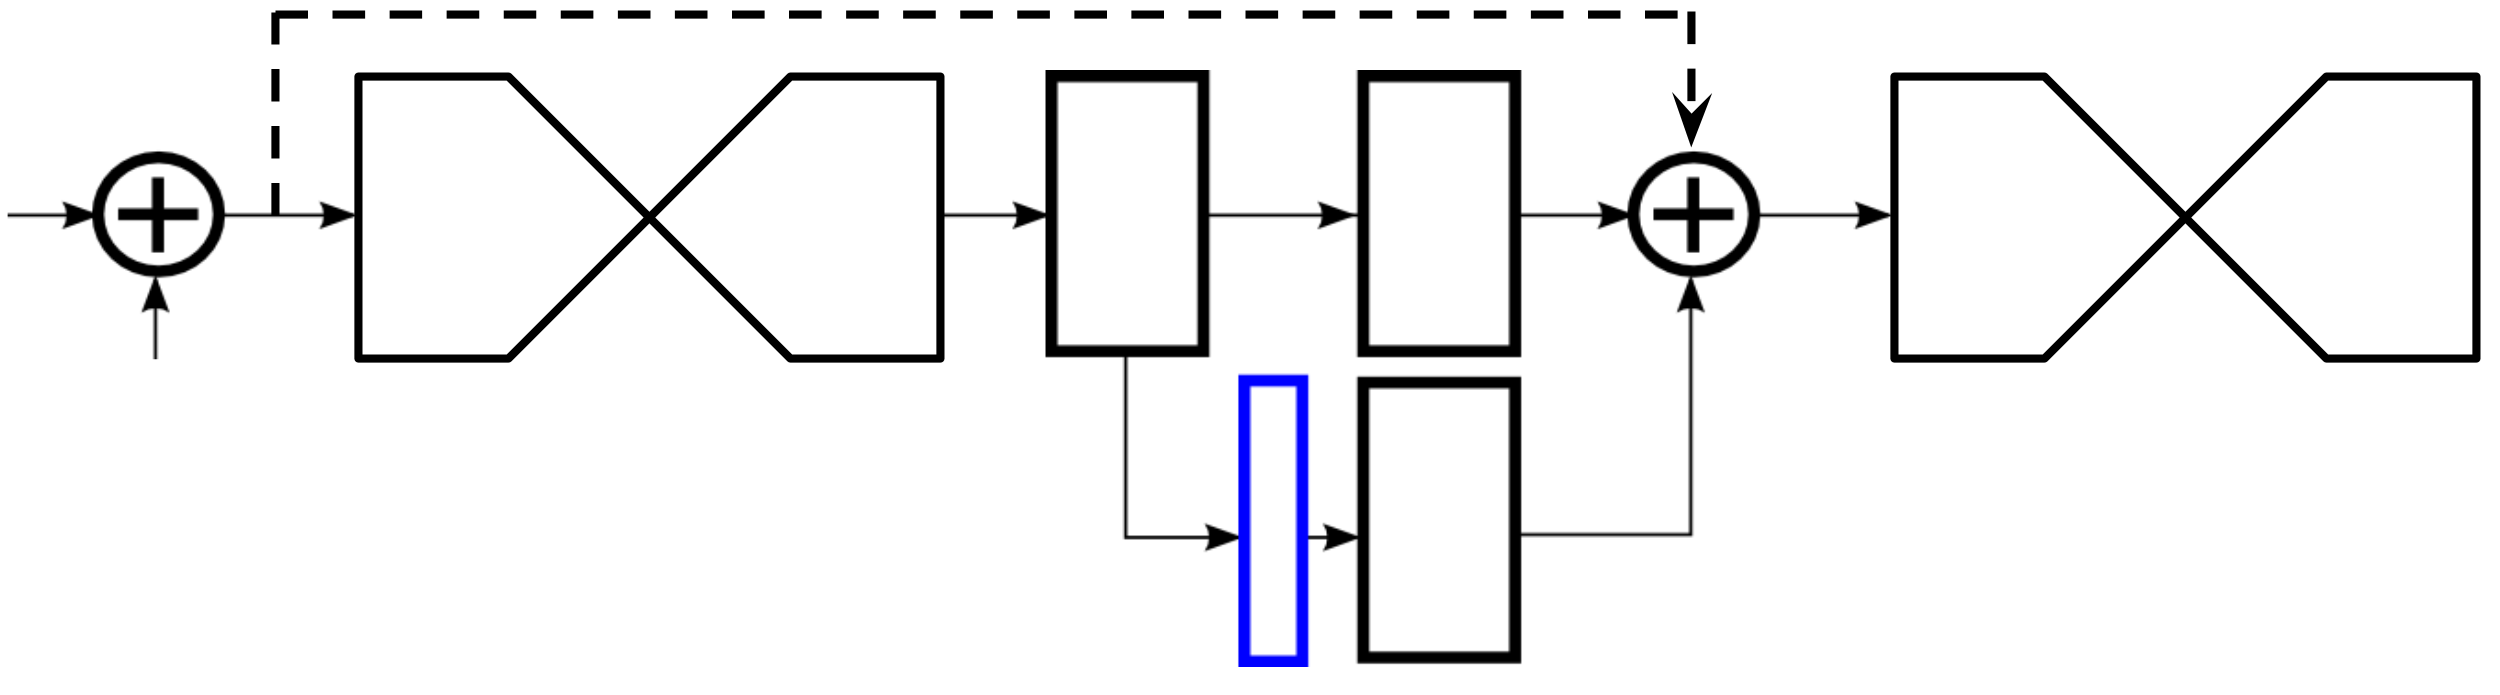
\includegraphics[width=0.95\linewidth]{images/stacked_hourglass.png}
    \caption[Architektura stacked hourglass sítě]{Schématické znázornění architektury \textit{stacked hourglass network} dle Newell et al. \cite{Newell2016}}
    \label{fig:stacked-hourglass}
\end{figure}

Pro detekci anatomických \textbf{klíčových bodů} (klíčových bodů) ve snímcích se uplatňují jak přístupy založené na segmentaci a následné extrakci bodů, tak i přímé detekční modely. V této práci je pro úlohu přímé lokalizace klíčových bodů využit přístup založený na architektuře \textbf{stacked hourglass network}. Tato architektura byla původně navržena pro odhad lidské pózy v obraze, tedy pro přesnou lokalizaci anatomicky definovaných bodů, a právě proto se dobře hodí i pro detekci referenčních bodů na RTG snímcích páteře \cite{Newell2016}.

Základním stavebním prvkem této architektury je tzv. \textbf{hourglass modul}. Jeho princip spočívá v tom, že síť nejprve v rámci \textit{bottom-up} části postupně snižuje prostorové rozlišení příznakových map pomocí poolingových nebo stridovaných konvolučních operací. Tím získává širší kontext a dokáže zachytit vztahy mezi vzdálenějšími strukturami v obraze. Následně v \textit{top-down} části dochází k opětovnému navyšování rozlišení, typicky pomocí upsamplingu, aby bylo možné obnovit jemnou prostorovou informaci potřebnou pro přesnou lokalizaci bodů. Důležitou součástí architektury jsou také \textbf{skip connections}, které propojují odpovídající úrovně při zmenšování a zvětšování rozlišení. Díky nim se kombinují globální kontextové informace s lokálními obrazovými detaily, což je zásadní zejména tehdy, když mají detekované body malý rozměr nebo leží na strukturách s neostrou hranicí \cite{Newell2016}.

Vlastnost, která odlišuje \textit{stacked hourglass} od jednodušších encoder-decoder architektur, spočívá v \textbf{řetězení několika hourglass modulů za sebou}. Každý modul vytváří vlastní odhad polohy klíčových bodů a následující modul tento odhad dále zpřesňuje. Síť tedy neprovádí lokalizaci pouze jednou, ale opakovaně se k ní vrací a v dalších průchodech koriguje dřívější nepřesnosti. Tento princip iterativního zpřesňování je v původní práci doplněn také o \textbf{intermediate supervision}, tedy pomocné ztrátové funkce na výstupech jednotlivých modulů. Díky tomu se model učí smysluplné reprezentace již v průběžných fázích sítě a lépe využívá víceúrovňové obrazové informace \cite{Newell2016}.

Výstupem stacked hourglass modelu obvykle nejsou přímo souřadnice bodů, ale \textbf{heatmapy} odpovídající jednotlivým klíčových bodů. Pro každý klíčový bod model predikuje jednu pravděpodobnostní mapu, v níž vysoké hodnoty označují pravděpodobnou polohu daného bodu. Během trénování se jako referenční výstup používají zpravidla Gaussovsky rozprostřené heatmapy se středem v anotované poloze bodu. Tento přístup je v úlohách přesné lokalizace výhodný, protože model neodhadne pouze jedinou dvojici souřadnic, ale celé prostorové rozložení pravděpodobnosti. Současné práce v medicínském zobrazování potvrzují, že \textbf{heatmap-based} metody patří mezi hlavní přístupy pro detekci klíčových bodů, zejména tam, kde je důležitá vysoká lokalizační přesnost a omezení chyb vznikajících při převodu mezi nízkým a vysokým rozlišením \cite{Zhang2024SRLD}.

Pro rentgenové snímky páteře je stacked hourglass vhodný zejména proto, že dokáže současně využít \textbf{globální uspořádání páteře} i \textbf{lokální tvar jednotlivých obratlů}. Při detekci rohů obratlových těl nebo jiných referenčních bodů totiž nestačí sledovat pouze malé okolí bodu, ale je nutné zohlednit i polohu vůči sousedním obratlům a celkové zakřivení páteře. Hourglass architektura tuto potřebu přirozeně naplňuje víceškálovým zpracováním obrazu a opakovanou refinací predikce. Výhodou je také to, že model lze učit přímo na lokalizační úlohu bez nutnosti následného odvozování bodů ze segmentačních masek.

V posledních letech byly hourglass architektury úspěšně použity i v medicínských radiografických úlohách. Nakarai et al. (2023) aplikovali hourglass síť s globální a lokální refinací pro automatický výpočet parametrů krční páteře z laterálních RTG snímků a ukázali, že tento přístup dosahuje dobré přesnosti i na externím validačním souboru \cite{Nakarai2023}. Ještě novější práce Häfliger et al. (2025) využila \textit{stacked hourglass neural network} pro automatickou detekci anatomických bodů na dlouhých RTG snímcích dolních končetin. Autoři ukázali, že i v podmínkách relativně malého trénovacího souboru může tento typ architektury poskytovat vysokou shodu s manuálním hodnocením odborníků \cite{Hafliger2025}. Tyto výsledky naznačují, že stacked hourglass zůstává i v současnosti prakticky relevantní architekturou pro úlohy přesné lokalizace anatomických klíčových bodů v medicínských snímcích.

Nevýhodou stacked hourglass modelů může být vyšší výpočetní náročnost oproti jednodušším sítím, protože opakované zpracování ve více modulech zvyšuje počet parametrů i dobu inference. Přesto však tento přístup představuje velmi vhodnou volbu pro úlohy, v nichž je rozhodující přesná lokalizace menšího počtu anatomicky významných bodů. V kontextu této práce je stacked hourglass architektura vhodná zejména proto, že umožňuje přímo detekovat referenční body potřebné pro následný výpočet klinických parametrů páteře, aniž by bylo nutné nejprve provádět segmentaci jednotlivých obratlů.

\chapter{Použité knihovny a frameworky}
\label{sec:libraries}

\section{Přehled}
Implementace, trénování i vyhodnocení neuronových sítí v této práci je realizováno pomocí knihovny \textbf{PyTorch} \cite{Paszke2019PyTorch}. Nadstavbou pro medicínské zobrazování je framework \textbf{MONAI}, který poskytuje hotové architektury, transformace i inferenční nástroje \cite{Cardoso2022MONAI}. Postprocessing, vizualizace a morfologické operace jsou realizovány pomocí knihoven \textbf{OpenCV} \cite{Bradski2000OpenCV}, \textbf{NumPy} \cite{Harris2020NumPy}, \textbf{scipy.ndimage} jako součásti knihovny \textbf{SciPy} \cite{Virtanen2020SciPy}, \textbf{scikit-image} \cite{VanDerWalt2014Skimage} a \textbf{Pillow} \cite{PillowDocs}. Projekt dále využívá vlastní nástroje v rámci modulu \texttt{Src}.


\section{Použité knihovny}

V implementaci byly využity jak obecné knihovny pro numerické výpočty a práci s obrazem, tak specializované frameworky pro hluboké učení a medicínské zobrazování. Jednotlivé knihovny v projektu neplní pouze podpůrnou roli, ale přímo zajišťují načítání dat, definici a trénování modelu, inferenci, postprocessing segmentačních masek i následnou extrakci anatomických klíčových bodů. Následující přehled proto neuvádí pouze obecný účel použitých nástrojů, ale také jejich konkrétní roli v implementovaných skriptech.

\subsection*{PyTorch}
PyTorch tvoří základ celé implementace neuronových sítí a experimentální pipeline. V projektu je využíván především pro reprezentaci dat ve formě tenzorů, přesun výpočtů na GPU, optimalizaci modelu a správu trénovacího procesu. Třídy \texttt{Dataset} a \texttt{DataLoader} z modulu \texttt{torch.utils.data} slouží k dávkovému načítání trénovacích a validačních dat, přičemž v třídě \texttt{AtlasDataset} jsou vstupní snímky a masky převáděny do formátu vhodného pro další transformace a zpracování modelem \cite{PyTorchDataLoader}. V souboru \texttt{atlas\_model\_multiclass\_patch.py} je \texttt{DataLoader} použit pro tvorbu trénovacích a validačních batchů a pro řízení náhodnosti při načítání dat pomocí definovaného seedování.

Další důležitou úlohou PyTorche je samotné trénování modelu. Ve skriptu \texttt{training\-\_new.py} jsou pomocí PyTorche realizovány dopředný průchod sítí, výpočet ztráty, zpětné šíření gradientu a aktualizace vah modelu. K optimalizaci parametrů je použit algoritmus \texttt{Adam}, zatímco řízení učicí rychlosti je zajištěno schedulery \texttt{ReduceLR\-OnPlateau} a \texttt{CosineAnnealing\-WarmRestarts}. Modul \texttt{torch.nn.functional} je v kódu využíván například pro převod predikovaných tříd na \textit{one-hot} reprezentaci pomocí \texttt{F.one\_hot}, což je následně potřeba při výpočtu Dice metriky po jednotlivých třídách. Funkce \texttt{torch.softmax} a \texttt{torch.argmax} jsou využity jak během validace, tak při inferenci k převodu výstupních logitů na finální segmentační predikci.

PyTorch je dále použit pro ukládání a načítání checkpointů modelu pomocí \texttt{torch\-.save} a \texttt{torch\-.load}, což umožňuje průběžné ukládání vah během trénování i následné znovunačtení modelu pro testování a inferenci. V souboru \texttt{training\_new.py} je navíc využit \texttt{SummaryWriter} z \texttt{torch.utils\-.tensorboard} pro zaznamenávání průběhu ztráty, Dice skóre a učicí rychlosti do TensorBoardu, což usnadňuje sledování konvergence modelu a porovnávání jednotlivých experimentů.

\subsection*{MONAI}
MONAI je specializovaná knihovna postavená nad PyTorch, určená pro vývoj metod hlubokého učení v medicínském zobrazování. V této práci představuje hlavní vrstvu nad základní PyTorch implementací a je využita jak při definici segmentačního modelu, tak při předzpracování dat, validaci a inferenci \cite{MONAIRepo,MONAISlidingWindowInferer}. Architektura segmentační sítě je převzata z modulu \texttt{monai.networks.nets}, konkrétně jde o třídu \texttt{UNet}, která je ve skriptech \texttt{atlas\_model.py}, \texttt{atlas\_model\-\_multiclass.py} a \texttt{atlas\_model\-\_multiclass\_patch.py} instanciována s parametry odpovídajícími 2D segmentaci krčních obratlů.

Významná role MONAI spočívá také v transformacích vstupních dat. Pomocí \texttt{\-Compose} jsou skládány celé transformační pipeline, které zahrnují například \texttt{\-Scale\-Intensityd}, \texttt{SpatialPadd}, \texttt{RandSpatialCropd}, \texttt{RandFlipd}, \texttt{RandRotate90d}, \texttt{Rand\-Zoomd}, \texttt{\-Rand\-Gaussian\-Noised} a \texttt{ToTensord}. Tyto transformace jsou využity při přípravě dat pro trénink i validaci a zajišťují sjednocení velikosti vstupů, augmentaci i převod do tenzorové reprezentace. Součástí pipeline je i vlastní transformace \texttt{Histogram\-Equalizationd}, která je implementována jako potomkem \texttt{MapTransform} a zapadá tak přímo do MONAI transformačního frameworku.

V trénovací i validační části je MONAI využit také pro vyhodnocení kvality segmentace. Ve skriptu \texttt{training\_new.py} se používá \texttt{DiceMetric} pro průběžné sledování úspěšnosti modelu na trénovacích i validačních datech. Ve skriptu \texttt{testing.py} jsou pak využity \texttt{DiceMetric} a \texttt{compute\_iou} pro výpočet Dice (vzorec \ref{eq:dice}) a IoU (vzorec \ref{eq:iou}) metrik po jednotlivých třídách i v průměru přes celý snímek.

Pro inferenci v plném rozlišení snímků je zásadní funkce \texttt{sliding\-\_window\-\_infere\-nce} (funkčnost vysvětlena v kapitole \ref{subsec:sliding_window}). Ta je použita jak ve validační smyčce v \texttt{training\-\_new.py}, tak zejména ve skriptu \texttt{inference.py}, kde umožňuje zpracovávat i větší rentgenové snímky po překrývajících se oknech fixní velikosti. Tento postup je důležitý z hlediska paměťových omezení GPU a současně umožňuje zachovat vyšší prostorové rozlišení vstupních dat bez nutnosti jejich agresivního zmenšování.

\subsection*{NumPy}
NumPy je základní knihovna pro numerické výpočty v jazyce Python a představuje standardní nástroj pro práci s vícerozměrnými poli a maticovými operacemi \cite{Harris2020NumPy}. V této práci je využívána napříč celou implementací zejména pro reprezentaci obrazových dat a masek, manipulaci s jejich rozměry, indexaci, prahování a další základní numerické operace potřebné při předzpracování dat, postprocessingu i vyhodnocení výsledků.


\subsection*{OpenCV}
OpenCV je open-source knihovna určená pro zpracování obrazu a počítačové vidění, která poskytuje širokou škálu nástrojů pro práci s rastrovými daty, geometrickými transformacemi, filtrací, segmentací i vizualizací \cite{Bradski2000OpenCV}. V této práci je využívána zejména pro načítání a ukládání obrazových dat, tvorbu vizualizačních výstupů, překryv segmentačních masek s původním RTG snímkem a pro dílčí operace nad obrazem a binárními maskami v rámci postprocessingu.


\subsection*{scipy.ndimage}
Modul \texttt{scipy.ndimage}, který je součástí knihovny SciPy, poskytuje nástroje pro zpracování vícerozměrných dat, zejména obrazů a objemových reprezentací \cite{Virtanen2020SciPy}. V této práci je využíván především v postprocessingu segmentačních výstupů, kde slouží k morfologickým operacím nad binárními maskami a k jejich následnému čištění a zpřesnění před další analýzou.

\subsection*{scikit-image}
Knihovna \texttt{scikit-image} je určena pro zpracování a analýzu obrazových dat v prostředí Pythonu a poskytuje nástroje pro segmentaci, měření vlastností oblastí i extrakci obrazových příznaků \cite{VanDerWalt2014Skimage}. V této práci je využívána především pro analýzu segmentačních masek, zejména pro identifikaci souvislých komponent, výpočet jejich základních geometrických vlastností a výběr oblastí odpovídajících jednotlivým anatomickým strukturám.

\subsection*{Pillow (PIL)}
Pillow je knihovna určená pro práci s rastrovými obrazovými soubory v jazyce Python a navazuje na původní Python Imaging Library \cite{PillowDocs}. V této práci slouží především k načítání a ukládání obrazových dat, převodům mezi obrazovou a numerickou reprezentací a k přípravě vizualizačních výstupů v běžných obrazových formátech.

\chapter{Extrakce klíčových bodů ze segmentační masky}
\label{chap:extraction}

Samotná segmentační maska sice poskytuje informaci o poloze a tvaru jednotlivých obratlů, pro výpočet sledovaných radiologických parametrů však sama o sobě nestačí. Klinické metriky, jako jsou sklon krycích plotének, segmentové úhly nebo Cobbův úhel C2--C7, je nutné odvozovat z přesně definovaných anatomických referenčních bodů. Z tohoto důvodu bylo po segmentaci obratlů nutné navrhnout postup, který z binárních masek automaticky extrahuje sadu klíčových bodů reprezentujících jednotlivé obratle.

Extrakce klíčových bodů ze segmentačních masek byla realizována v několika fázích, implementovaných ve skriptu \texttt{extraction.py}\footnote{Zdrojový kód je dostupný na GitHubu: \url{https://github.com/JaroslavRadimsky/vertebra_segmentation_and_keypoint_extraction}}. Cílem bylo získat 23 bodů popisujících pozice obratlů C2 až C7.


\section{Výběr hlavní kontury a převod barevné masky}
\label{sec:mask_color_conversion}

Výstup segmentačního modelu byl pro účely uložení, vizualizace a následného zpracování reprezentován jako barevně kódovaná maska, v níž byly jednotlivé obratle odlišeny specifickými barvami v prostoru BGR. Přestože segmentační model interně pracuje s binárními nebo vícekanálovými pravděpodobnostními mapami, pro navazující postprocessing bylo výhodné převést výstup do jednotné obrazové reprezentace, která umožňuje snadnou vizuální kontrolu i jednotné zpracování predikcí a referenčních masek. Pro další extrakci kontur však bylo nutné tyto barevné oblasti převést zpět na binární masky jednotlivých tříd. Tento převod zajišťuje funkce \texttt{mask\_from\_color} ve skriptu \texttt{extraction.py}. V budoucích verzích programu se bude pracovat rovnou se získanými segmentačními maskami přímo z modelu.

Funkce \texttt{mask\_from\_color} přijímá jako vstup barevný obraz a cílovou barvu ve formátu BGR, například \texttt{(0, 255, 0)} pro zelenou. Výsledkem je binární maska, kde jsou pixely odpovídající zadané barvě nastaveny na hodnotu \texttt{255} (bílá), zatímco ostatní jsou \texttt{0} (černá). Maska může být vytvořena buď přesnou shodou barev, nebo s definovanou tolerancí, která umožňuje zahrnout i pixely s drobnou barevnou odchylkou.

Funkce obsahuje dvě větve:

\begin{itemize}
  \item Pokud je tolerance nulová (\texttt{tol = 0}), je provedena přesná shoda – porovnávají se všechny tři barevné kanály (B, G, R) a binární maska je vytvořena logickou konjunkcí přesných rovností.
  \item Pokud je tolerance větší než nula, jsou pro každý kanál vypočteny dolní a horní hranice (\texttt{np.clip(color - tol, 0, 255)} a \texttt{np.clip(color + tol, 0, 255)}), a následně je použita funkce \texttt{cv2.inRange}, která vytvoří binární masku zahrnující i „přibližně odpovídající“ pixely.
\end{itemize}

Tato flexibilita umožňuje extrakci i při drobných odchylkách způsobených kompresí, interpolací nebo exportem masek.

Výstupní binární masky jsou následně použity pro extrakci kontur. Každé třídě je přiřazena její největší kontura, získaná pomocí funkce \texttt{main\_contour}. Tato funkce volá \texttt{cv2.findContours} a vybírá konturu (proměnná \texttt{contour}) s největší plochou, což odpovídá hlavnímu tělu obratle.

\section{Seřazení segmentovaných oblastí}
Každá extrahovaná oblast (odpovídající jednomu obratli) je reprezentována maskou a jejím centroidem, který je spočítán funkcí \texttt{centroid\_of\_mask}. Oblasti jsou následně seřazeny podle vertikální souřadnice centroidu, aby odpovídaly anatomickému pořadí C2--C7 (shora dolů).

\section{Extrakce bodů pro obratel C2}
Obratel C2 je v použitém datasetu anotován pouze třemi body (viditelné na obrázku \ref{fig:c2_c3_labeled}) a je zpracován odlišně. 

\begin{figure}
    \centering
    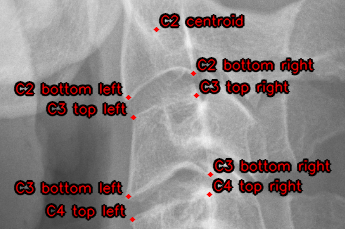
\includegraphics[width=0.5\linewidth]{images/c2_c3_labeled.png}
    \caption{Úkázka anotovaných bodů na obratlech C2 a C3}
    \label{fig:c2_c3_labeled}
\end{figure}

Nejprve se funkce \texttt{approx\_poly\_n} pokusí aproximovat konturu na tři vrcholy. Uvnitř se využívá funkce \texttt{cv2.approxPolyN}, která přijímá jako vstup konturu (např. výstup z \texttt{cv2.findContours}) a cílový počet vrcholů $n\_vertices$. Uvnitř funkce se volá:
\begin{verbatim}
approx = cv2.approxPolyDP(contour, epsilon, True)
\end{verbatim}
kde \texttt{epsilon} je parametr určující maximální odchylku od původní kontury. Hodnota \texttt{epsilon} se typicky zvyšuje v krocích (např. od 0.01 do 0.1 násobku délky kontury), dokud výstupní počet bodů neodpovídá požadovanému $n$.

Pokud tato aproximace selže, použije se záložní strategie složená ze dvou funkcí:

\begin{itemize}
  \item \texttt{bottom\_edge\_endpoints\_from\_contour} vybere levý a pravý dolní roh. Výpočet se omezuje na dolní pás kontury (50~\% výšky) a z něj se vyberou dva krajní body podél osy $x$.
  \item \texttt{apex\_top\_point\_from\_contour} určuje apex\footnote{V anatomii se termín apex používá pro označení vrcholu nebo nejvyššího bodu určité struktury. V tomto případě jde o nejvyšší bod identifikované oblasti obratle.} kontury jako průměr všech blízkých v rozsahu definovaném parametrem (počet pixelů od nejvyššího bodu na ose $y$).
\end{itemize}

Získané body jsou vylepšeny subpixelovou korekcí pomocí \texttt{refine\_subpix}, která využívá funkci \texttt{cv2.cornerSubPix}. Princip subpixelového zpřesnění vychází z analýzy změn jasových hodnot v okolí počátečně odhadnutého bodu. Předpokládejme, že \(q\) je počáteční poloha rohu a \(p\) je některý bod v jeho okolí. Pro správně určenou polohu rohu platí, že gradient obrazu v bodě \(p\) je kolmý na vektor \(q - p\), takže jejich skalární součin je přibližně nulový. Tento vztah se sestaví pro více bodů v okolí bodu \(q\), čímž vznikne soustava rovnic, jejímž řešením se získá přesnější odhad polohy rohu.

Nově vypočtená poloha se následně použije jako další počáteční odhad a celý postup se opakuje iterativně, dokud není splněna zadaná podmínka ukončení. Díky tomu lze určit polohu bodu s přesností vyšší, než odpovídá rozlišení jednoho pixelu.

Body jsou následně seřazeny jako: levý dolní, pravý dolní, apex (horní) pomocí funkce \texttt{order\_triangle\_bl\_br\_apex}.

Použité parametry funkcí jsou vypsané v tabulce \ref{tab:c2_extraction_params}.

\begin{table}[H]
\centering
\caption{Parametry funkcí používaných při extrakci bodů obratle C2.}
\label{tab:c2_extraction_params}
\begin{tabular}{p{5.2cm} p{8cm}}
\toprule
\textbf{Funkce} & \textbf{Parametry (použité hodnoty)} \\
\midrule
\texttt{approx\_poly\_n} & \texttt{contour: contour}, \texttt{n\_vertices: 3} \\
\texttt{cv2.approxPolyDP} & 
\begin{minipage}[t]{8cm}
\small
\texttt{contour: contour}, \\
\texttt{epsilon: np.linspace(...) * arcLength}, \\
\texttt{closed: True} 
\end{minipage} \\
\texttt{bottom\_edge\_endpoints \_from\_contour} & \texttt{band\_frac: 0.5}, \texttt{min\_band\_px: 8} \\
\texttt{apex\_top\_poin t\_from\_contour} & \texttt{y\_tol: 3} \\
\texttt{refine\_subpix} & \texttt{mask: mask}, \texttt{corners: pts}, \texttt{win: 7} \\
\texttt{cv2.cornerSubPix} & 
\begin{minipage}[t]{8cm}
\small
\texttt{image: cv2.GaussianBlur(mask\_u8,\- (5, 5), 0)}\\
\texttt{corners:\- corners\_xy.astype(np.float32)\-.reshape(-1, 1, 2)}\\
\texttt{winSize: (7, 7)}, \texttt{zeroZone: (-1, -1)}\\
\texttt{criteria: (cv2.TERM\_CRITERIA\_EPS +}\\
\texttt{cv2.TERM\_CRITERIA\_MAX\_ITER, 50, 1e-4)}
\end{minipage} \\
\texttt{order\_triangle \_bl\_br\_apex} & \texttt{pts\_xy: approx\_poly\_n(cnt, 3)} \\
\bottomrule
\end{tabular}
\end{table}

\section{Extrakce rohů u obratlů C3--C7}
U ostatních obratlů jsou anotovány čtyři body a to rohy obratlů (viditelné na obrázku~\ref{fig:c2_c3_labeled}). Navržený postup jejich získání vypadá následovně:

\begin{itemize}
  \item Funkce \texttt{approx\_quad} hledá čtyřúhelníkové přiblížení kontury pomocí polygonální aproximace. Pokud polygonální aproximace selže, postupuje se alternativně přes metodu \texttt{cv2.minAreaRect}, která odhaduje pomocí obdelníku.
  \item Pokud jsou rohy příliš blízko nebo zkreslené, funkce \texttt{merge\_close\_points} a \texttt{quad\_is\_valid} slouží ke kontrole a opravě.
  \item Rohy jsou doladěny pomocí \texttt{refine\_subpix}, stejně jako u obratle C2. Subpixelová korekce zajišťuje vyšší přesnost rohů, což má pozitivní vliv na následné klinické měření metrik.
  \item Následně jsou body seřazeny podle pozice dolních bodů předchozího obratle (funkce \texttt{order\_quad\_from\_previous\_bottom}). Například tedy levý horní roh obratle C4 bude bod z kontury, který je nejbližší levému dolnímu rohu obratle C5.
\end{itemize}

\begin{table}[H]
\centering
\caption{Parametry funkcí používaných při extrakci rohů obratlů C3--C7.}
\label{tab:c3_c7_extraction_params}
\begin{tabular}{p{5.2cm} p{8cm}}
\toprule
\textbf{Funkce} & \textbf{Parametry (použité hodnoty)} \\
\midrule
\texttt{approx\_quad} & \texttt{contour: contour} \\
\texttt{merge\_close\_points} & \texttt{pts: approx}, \texttt{merge\_dist: 6.0} \\
\texttt{quad\_is\_valid} & \texttt{pts: quad}, \texttt{min\_pair\_dist: 8.0}, \texttt{min\_area: 50.0}, \texttt{min\_edge: 6.0} \\
\texttt{cv2.minAreaRect} & \texttt{points: cv2.convexHull(contour)} \\
\texttt{cv2.boxPoints} & \texttt{rect: cv2.minAreaRect(...)} \\
\texttt{refine\_subpix} & \texttt{mask: vertebra mask}, \texttt{corners: quad}, \texttt{win: 7} \\
\texttt{order\_quad \_from\_previous\_bottom} & \texttt{pts\_xy: quad}, \texttt{prev\_bl: np.ndarray}, \texttt{prev\_br: np.ndarray} \\
\texttt{order\_quad\_clockwise (fallback)} & \texttt{pts\_xy: np.ndarray} \\
\bottomrule
\end{tabular}
\end{table}

Původně byly body seřazovány pouze na základě jejich souřadnic. Tento přístup však musel být nahrazen, protože u některých snímků (zejména při výrazném předklonu nebo záklonu krční páteře) docházelo k takovému natočení obratlů, že jeden ze spodních rohů se nacházel výše než horní. To vedlo k chybnému určení pořadí rohů (ukázka na obrázku \ref{fig:problematic_angle}) a následně k výrazným odchylkám při výpočtu metrik.

\begin{figure}
    \centering
    \includegraphics[width=0.5\linewidth]{images/problematic_angle.png}
    \caption{Ukázka chybné extrakce z důvodu velkého náklonu obratle}
    \label{fig:problematic_angle}
\end{figure}

\section{Výstup a formát JSON}
Každý detekovaný bod je zapsán do JSON ve formátu LabelMe pomocí funkce \texttt{labelme\-\_point}. Výsledný soubor generuje funkce \texttt{build\_labelme\_json}, který zahrnuje jméno souboru, rozměry obrazu a pole bodů.

Níže je ukázka výstupu JSON pro jeden obratel (C2):

\begin{verbatim}
{
  "shapes": [
    {
      "label": "C2 bottom left",
      "points": [[261.31, 342.77]],
      "shape_type": "point"
    },
    {
      "label": "C2 bottom right",
      "points": [[326.30, 318.75]],
      "shape_type": "point"
    },
    {
      "label": "C2 centroid",
      "points": [[289.37, 275.07]],
      "shape_type": "point"
    }
  ]
}
\end{verbatim}

Celý proces pro jednotlivý snímek je realizován ve funkci \texttt{process\_one\_mask}, která kombinuje všechny kroky výše a vytváří výstupní anotaci.

\chapter{Popis provedených experimentů}
\label{chap:workflow}

\section{Použitý dataset}

V této práci byl využit veřejně dostupný dataset \textbf{Cervical Spine X-ray Atlas (CSXA)}\cite{Ran2024}, publikovaný v roce 2024. Tento dataset obsahuje \textbf{4\,963} rentgenových snímků krční páteře ve formátu PNG. Ke každému snímku je přiložen soubor s anotací ve formátu JSON.

Každý obrázek byl ručně anotován sadou \textbf{23 anatomických klíčových bodů}, které zahrnují centroid a dva body dolní krycí plochy C2 a rohové body obratlů C3--C7.. Anotace byly třikrát ověřeny různými experty a validovány jak ručně, tak skriptem kontrolujícím úplnost a konzistenci.\cite{Ran2024}
Bohužel dataset i přes ověřované anotace obsahuje chybně anotované snímky (objevené při experimentování v rámci této práce), které byly v této práci opraveny (chybné anotace ručně změneny) za účelem nezkreslených výsledků.

Dataset je k dispozici na GitHubu\footnote{\url{https://github.com/yran888/CSXA-dataset}} a je archivován v úložišti Science Data Bank\footnote{\url{https://doi.org/10.57760/sciencedb.15391}}.

\section{Použité metriky hodnocení}
Pro trénování segmentačního modelu byly využity dvě běžně používané metriky: Dice koeficient a Intersection over Union (IoU). Dice koeficient je metrika překryvu definovaná jako:
\begin{equation}
\text{Dice} = \frac{2|A \cap B|}{|A| + |B|}
\label{eq:dice}
\end{equation}
kde $A$ je predikovaná maska a $B$ je referenční maska. IoU je pak poměr průniku a sjednocení těchto oblastí:
\begin{equation}
\operatorname{IoU} = \frac{|A \cap B|}{|A \cup B|}
\label{eq:iou}
\end{equation}

\begin{samepage}
Metriky byly v této práci počítány pomocí tříd \texttt{DiceMetric} a \texttt{IoUMetric} z frameworku MONAI \cite{MONAIRepo}.

Pro celkové zhodnocení výstupů a relevance vůči klinické praxi se však využívají specializované metriky určené k hodnocení stability krční páteře. Tyto metriky jsou popsány podrobně v kapitole \ref{sec:metrics}.
\end{samepage}

\section{Segmentační přístup}
\label{sec:segmentation}

\subsection{Trénink segmentačního modelu}

Segmentace obratlů byla řešena pomocí architektury \textbf{U-Net} implementované v knihovně MONAI. Vstupem jsou RGB snímky (3 kanály), výstupem je sedmikanálová mapa odpovídající šesti obratlům (C2–C7) a pozadí. Parametry modelu jsou popsány v tabulce \ref{tab:unet_arch_train}.

\begin{table}[H]
\centering
\caption{Parametry segmentačního modelu a trénovací konfigurace.}
\label{tab:unet_arch_train}
\begin{tabular}{p{5.2cm} p{8cm}}
\toprule
\textbf{Parametr} & \textbf{Hodnota} \\
\midrule
Vstupní kanály & 3 (RGB) \\
Výstupní kanály & 7 (C2–C7 + pozadí) \\
Počet úrovní (hloubka) & 5 \\
Kanály v jednotlivých úrovních & (16, 32, 64, 128, 256) \\
Downsampling strides & (2, 2, 2, 2) \\
Aktivační funkce & ReLU \\
Normalizace & výchozí konfigurace MONAI \\
Reziduální bloky & 2 na každé úrovni \\
Optimalizátor & Adam \\
Počáteční learning rate & 0.01 \\
Scheduler & CosineAnnealingWarmRestarts \cite{Loshchilov2017} (T\textsubscript{0}=5, T\textsubscript{mult}=2, $\eta_{\min}=10^{-8}$) \\
Ztrátová funkce & DiceCELoss (Dice + Cross-Entropy) \\
Počet epoch & 600 \\
\bottomrule
\end{tabular}
\end{table}

Model je vytvořen funkcí \texttt{UNet(...)}, přímo ve skriptu \texttt{atlas\_model\-\_multiclass\-\_patch.py} .

\subsection*{Patch-based trénink}

Vzhledem k vysokému rozlišení vstupních rentgenových snímků a relativně malé velikosti cílových struktur (obratlů) by použití celých obrazů během tréninku vedlo k neefektivnímu využití výpočetních prostředků i paměti GPU. Případně by z důvodů úspory paměti musel být obrázek přeškálován na nižší rozlišení. Z tohoto důvodu byl zvolen přístup tzv. \textbf{patch-based training}, kdy se model učí pouze na menších náhodně vyříznutých oblastech obrazu (patchech) o velikosti 512×512 pixelů. Každý vstupní snímek je v rámci jedné epochy reprezentován 20 náhodně vybranými výřezy. Tento způsob tréninku má několik výhod.

První výhodou je výrazné snížení paměťové náročnosti, protože jednotlivé patche obsahují pouze lokální informaci, a lze je zpracovávat ve větší dávce nebo s vyšším rozlišením než celé obrazy. Dále tento přístup zvyšuje datovou variabilitu, protože během tréninku jsou z každého obrázku vybírány různé části. Model se tak naučí rozpoznávat obratle v různých pozicích, s různým okolím a úrovní ořezu, což přispívá k lepší generalizaci. V neposlední řadě patch-based trénink eliminuje riziko přeučení na globální kontext snímku (například fixní polohu páteře vůči rozměrům obrazu), protože vstupy jsou vždy jen lokální.

Technicky je tento přístup realizován v konstruktoru třídy \texttt{AtlasDataset} v souboru \texttt{atlas\_dataset\_patch.py}, kde je nastaven parametr \texttt{patches\_per\_image=20}. Náhodné výřezy jsou generovány pomocí transformační komponenty \texttt{RandSpatialCropd} z knihovny MONAI, která zajišťuje, že každý patch bude rozměrově konzistentní a bude pocházet z náhodně zvoleného místa na vstupním snímku.

Celkově tak patch-based strategie umožňuje efektivnější trénování modelu, podporuje robustní učení na různorodých výřezech a zároveň poskytuje jistou míru augmentace bez nutnosti rozšiřovat původní dataset.

\newpage
\subsection*{Tréninkové transformace}

Transformační pipeline použitá při tréninku je popsána v tabulce \ref{tab:train_transforms}.

\begin{table}[H]
\centering
\caption{Tréninkové transformační kroky a jejich parametry.}
\label{tab:train_transforms}
\small
\begin{tabular}{p{3.5cm} p{5cm} p{5.5cm}}
\toprule
\textbf{Transformace} & \textbf{Třída (MONAI)} & \textbf{Hlavní parametry} \\
\midrule
Histogramová equalizace & \texttt{HistogramEqualizationd} (custom) & \texttt{keys=["image"]} \\
Normalizace intenzity & \texttt{ScaleIntensityd} & \texttt{keys=["image"]} \\
Padding na min. velikost & \texttt{SpatialPadd} & \texttt{keys=["image", "label"]}, \texttt{spatial\_size=(512, 512)} \\
Náhodné oříznutí (patch) & \texttt{RandSpatialCropd} & \texttt{keys=["image", "label"]}, \texttt{roi\_size=(512, 512)}, \texttt{random\_size=False} \\
Horizontální flip & \texttt{RandFlipd} & \texttt{keys=["image", "label"]}, \texttt{spatial\_axis=0}, \texttt{prob=0.5} \\
Vertikální flip & \texttt{RandFlipd} & \texttt{keys=["image", "label"]}, \texttt{spatial\_axis=1}, \texttt{prob=0.5} \\
Náhodná rotace o 90° & \texttt{RandRotate90d} & \texttt{keys=["image", "label"]}, \texttt{prob=0.5}, \texttt{max\_k=3} \\
Náhodný zoom & \texttt{RandZoomd} & \texttt{keys=["image", "label"]}, \texttt{min\_zoom=0.9}, \texttt{max\_zoom=1.1}, \texttt{prob=0.3} \\
Přidání gaussovského šumu & \texttt{RandGaussianNoised} & \texttt{keys=["image"]}, \texttt{prob=0.2} \\
Převod na tensor & \texttt{ToTensord} & \texttt{keys=["image", "label"]} \\
\bottomrule
\end{tabular}
\end{table}

\subsection*{Trénovací smyčka}

Trénink segmentačního modelu probíhá ve funkci \texttt{training\_loop}, která řídí jednotlivé epochy, vyhodnocení metrik a ukládání checkpointů. Optimalizace je zajištěna pomocí algoritmu \texttt{Adam}, jehož počáteční learning rate je nastaven na hodnotu 0.01. Aby se zamezilo přetrénování a podpořila stabilní konvergence, je použita ztrátová funkce \texttt{DiceCELoss}, což je implementace v knihovně MONAI kombinující Dice koeficient a klasickou vícetřídovou cross-entropy ztrátu. Dice složka optimalizuje podobnost predikované a referenční masky na úrovni celé segmentované oblasti, a je tak vhodná pro zachování správného tvaru a rozsahu objektu, zatímco cross-entropy složka působí na úrovni jednotlivých pixelů, kde penalizuje chybné klasifikace a doplňuje Dice loss o detailnější lokální informaci.

Trénink probíhal po dobu 600 epoch na grafické kartě NVIDIA A30. Pro efektivní řízení hodnoty learning rate v průběhu trénování je využit scheduler typu \break \texttt{\detokenize{CosineAnnealingWarmRestarts}} \cite{Loshchilov2017}, který periodicky snižuje learning rate podle kosinusového průběhu. V rámci jednoho cyklu je hodnota learning rate dána vztahem:
\begin{equation}
\eta_t = \eta_{\min} + \frac{1}{2}\left(\eta_{\max} - \eta_{\min}\right)\left(1 + \cos\left(\pi \frac{T_{cur}}{T_i}\right)\right),
\end{equation}
kde $\eta_t$ označuje aktuální learning rate, $\eta_{\max}$ je počáteční hodnota learning rate v daném cyklu, $\eta_{\min}$ je minimální hodnota learning rate, $T_{cur}$ je počet epoch od posledního restartu a $T_i$ je délka aktuálního cyklu. Po dosažení konce cyklu dojde k restartu scheduleru a learning rate se vrátí na vyšší hodnotu.

V implementaci je tento scheduler nakonfigurován s parametry $T_0 = 5$ a $T_{mult} = 2$, což znamená, že první restart nastává po 5 epochách a každé další období se zdvojnásobuje (5, 10, 20, \dots). Minimální hodnota learning rate je nastavena na $\eta_{\text{min}} = 10^{-8}$.


\begin{figure}
    \centering
    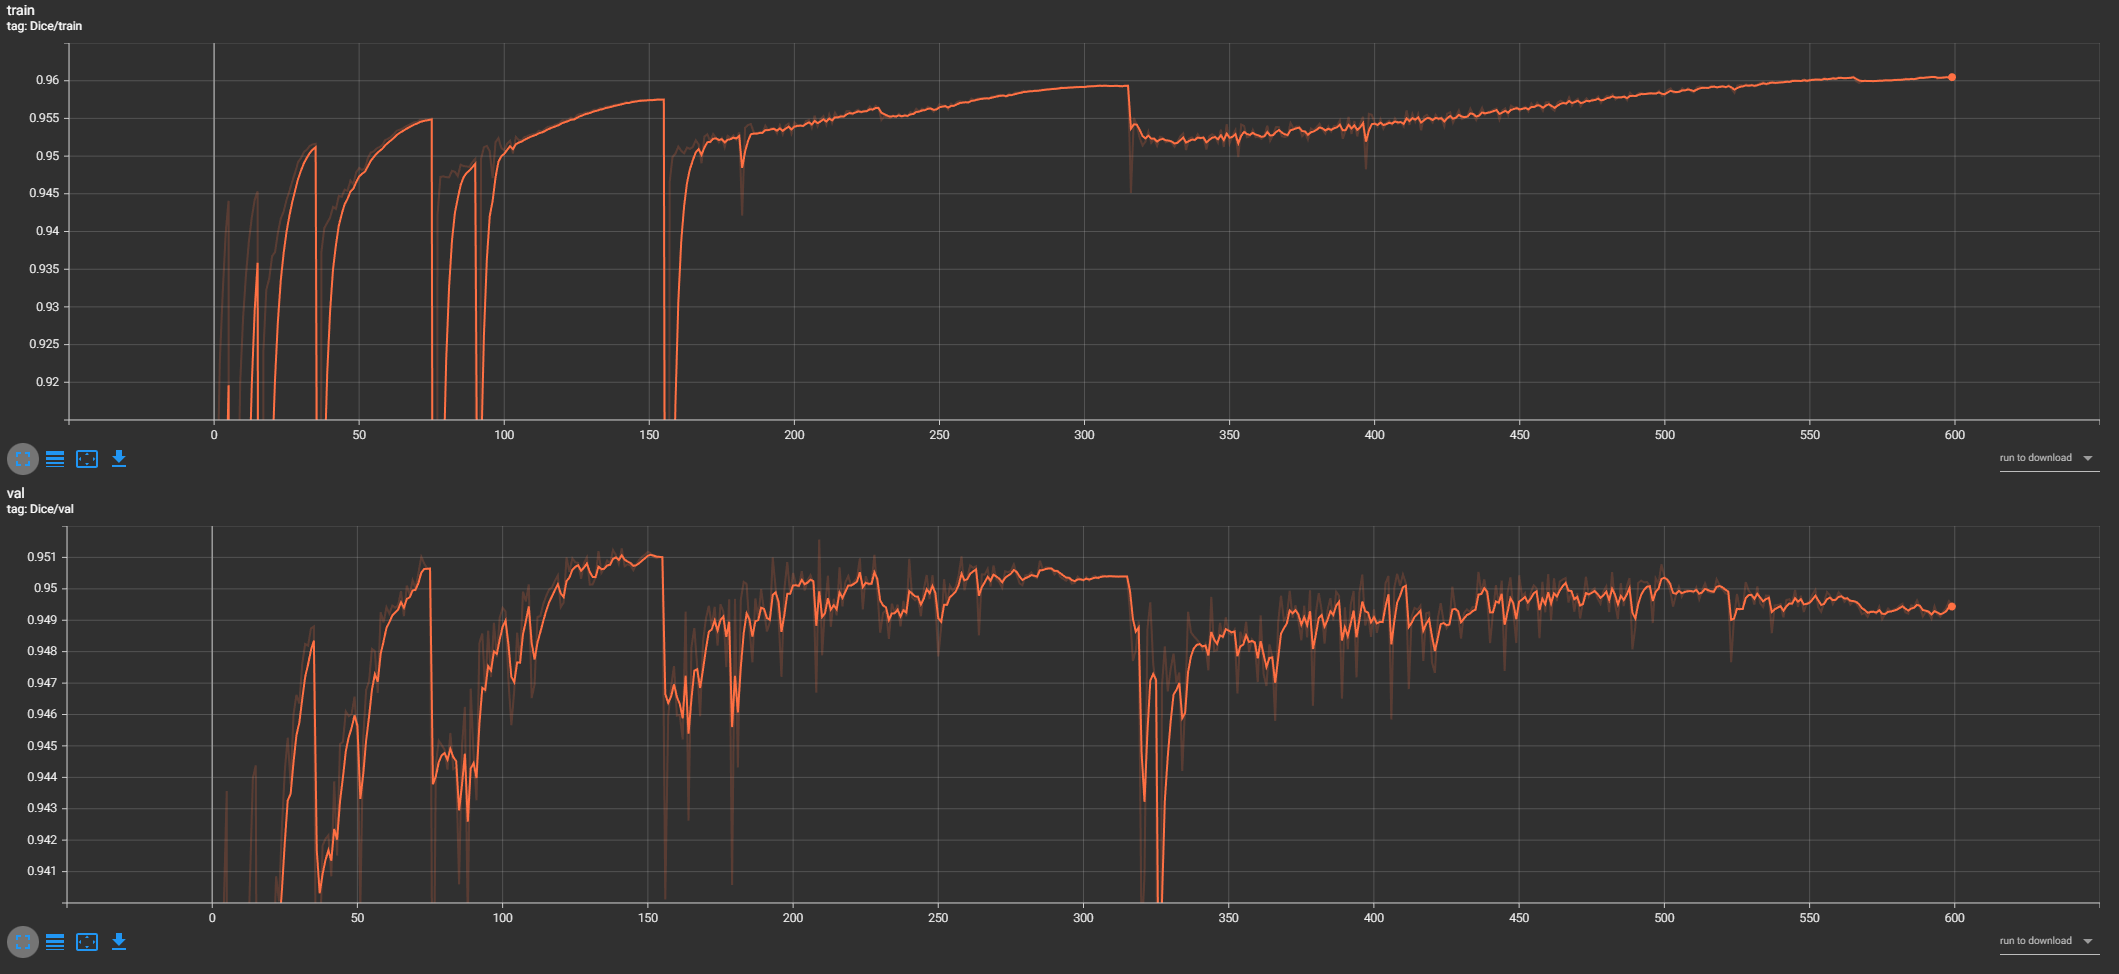
\includegraphics[width=1\linewidth]{images/Dice.png}
    \caption{Průběh metriky Dice trénovaného modelu (nahoře na trénovacích datech, dole na validačních)}
    \label{fig:Dice}
\end{figure}

\begin{figure}
    \centering
    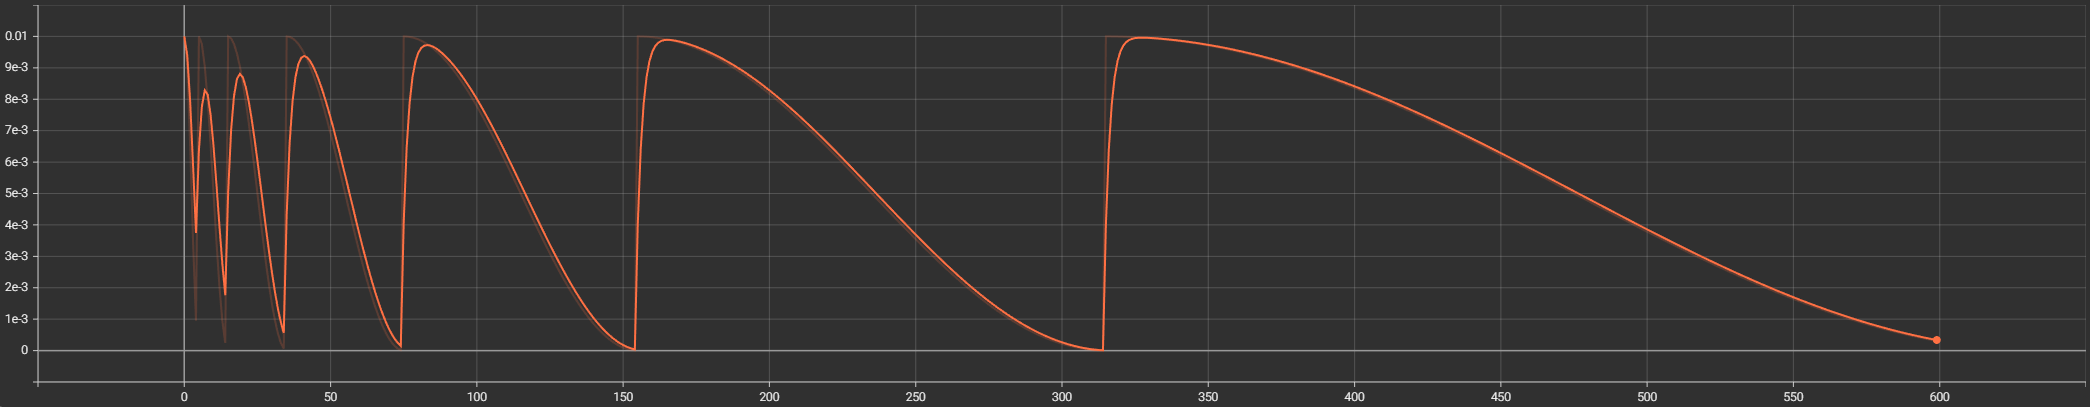
\includegraphics[width=1\linewidth]{images/LR.png}
    \caption{Průběh Learning rate trénovaného modelu}
    \label{fig:LR}
\end{figure}

Tento typ scheduleru umožňuje modelu opakovaně procházet fázemi rychlé a pomalé aktualizace, což může vést k lepší generalizaci – model se v pozdějších fázích tréninku vyhne „zamrznutí“ v lokálním minimu. Zároveň pomáhá stabilizovat učení při kombinaci s náhodnými augmentacemi a patch-based tréninkem, protože efektivně řídí rozsah úprav vah v různých fázích tréninku.

Celá strategie plánování learning rate je implementována v souboru \break \texttt{atlas\_model\_multiclass\_patch.py} ve funkci \texttt{get\_scheduler}.

\subsection*{Inference a sliding window}
\label{subsec:sliding_window}

Při inferenci je použit přístup \textbf{sliding window inference}, který umožňuje zpracování i větších snímků, než je trénovací velikost (512×512). Tento přístup spočívá v rozdělení vstupního obrazu na menší překrývající se oblasti (okna), které odpovídají velikosti vstupu modelu. Každé okno je následně zpracováno samostatně neuronovou sítí a výsledné predikce jsou zpětně skládány do výsledné výstupní mapy.

Klíčovým aspektem této metody je \textbf{překryv oken}, který zajišťuje, že každý pixel obrazu je predikován vícekrát z různých kontextů. To je důležité zejména pro oblasti poblíž hranic oken, kde by jinak mohlo docházet k artefaktům způsobeným omezeným zorným polem modelu.

Při skládání výsledků z jednotlivých oken se používá \textbf{vážené průměrování predikcí}. Každému pixelu v rámci okna je přiřazena váha (typicky vyšší ve středu okna a nižší u okrajů, např. pomocí gaussovského okna), aby se minimalizoval vliv méně spolehlivých predikcí na hranách. Výsledná hodnota pixelu ve finální mapě je pak získána jako průměr všech predikcí, které na danou pozici přispěly, vážený těmito koeficienty.

Tento postup umožňuje efektivní práci s pamětí, protože model nikdy nezpracovává celý obraz najednou. Nevýhodou je vyšší výpočetní náročnost způsobená opakovaným zpracováním překrývajících se oblastí.

\begin{figure}
    \centering
    \includegraphics[width=0.5\linewidth]{images/sliding_window_inference.png}
    \caption{Ukázka inference pomocí metody sliding window}
    \label{fig:sw_inference}
\end{figure}

Tento přístup je implementován pomocí funkce \texttt{sliding\-\_window\-\_inference} z kni\-hovny MONAI a je využit ve funkci \texttt{run\_inference\_on\-\_image\_sw} ve skriptu \texttt{infe\-rence.py}.

\subsection{Postprocessing segmentačních masek}

Po inferenci probíhá víceúrovňový postprocessing masky. Celý proces je implementován ve funkcích \texttt{postprocess\_mask} a \texttt{clean\_class} v souboru \texttt{inference.py} . Kroky jsou následující:

\begin{enumerate}
  \item \textbf{Práh jistoty:} Pomocí predikované softmax pravděpodobnosti je určen práh jistoty \texttt{conf\_thresh} (defaultně 0.5). Všechny pixely s maximální pravděpodobností nižší než tento práh jsou přepsány na třídu pozadí (0). Tento krok je realizován ve funkci \texttt{run\_inference\_on\_image\_sw}.

  \item \textbf{Čištění tříd:} Každá třída (1–6) je zpracována zvlášť funkcí \texttt{clean\_class}, která obsahuje následující podkroky:
  \begin{enumerate}
    \item \textit{Odstranění malých komponent:} Pomocí \texttt{skimage.measure.label} a \texttt{region\-props} se detekují jednotlivé komponenty a všechny s plochou menší než 500~px (\texttt{min\_size=500}, hodnota nastavena exeprimentálně) jsou odstraněny.
    \item \textit{Zachování největší komponenty:} Zbývající komponenty se znovu analyzují a ponechá se pouze ta s největší plochou.
    \item \textit{Morfologické operace:} Na binární masku největší komponenty se aplikuje:
    \begin{itemize}
      \item \texttt{binary\_opening} se strukturálním elementem \texttt{np.ones((3,3))} -- odstranění malých výčnělků,
      \item \texttt{binary\_closing} se stejným elementem -- vyplnění malých otvorů,
      \item \texttt{binary\_fill\_holes} -- finální vyplnění vnitřních děr.
    \end{itemize}
  \end{enumerate}

  Příklad postprocessingu lze vidět na obrázku \ref{fig:postprocessing}.

  \item \textbf{Přerelabelování tříd (volitelné):} Pokud je přepínač \texttt{apply\_relabel=True}, třídy 1–6 jsou seřazeny podle vertikální pozice jejich centroidu (odshora dolů). Tento krok je realizován funkcí \texttt{relabel\_by\_vertical\_position}, která opět využívá centroidy komponent získané přes \texttt{regionprops}. Cílem je zajistit konzistentní anatomické pořadí obratlů nezávisle na případném záměně tříd modelem.
\end{enumerate}

Tento postprocessing zvyšuje konzistenci výstupních masek, zajišťuje hladké okraje a minimalizuje chyby v pořadí obratlů, což je klíčové pro následnou extrakci klíčových bodů.

\begin{figure}
    \centering
    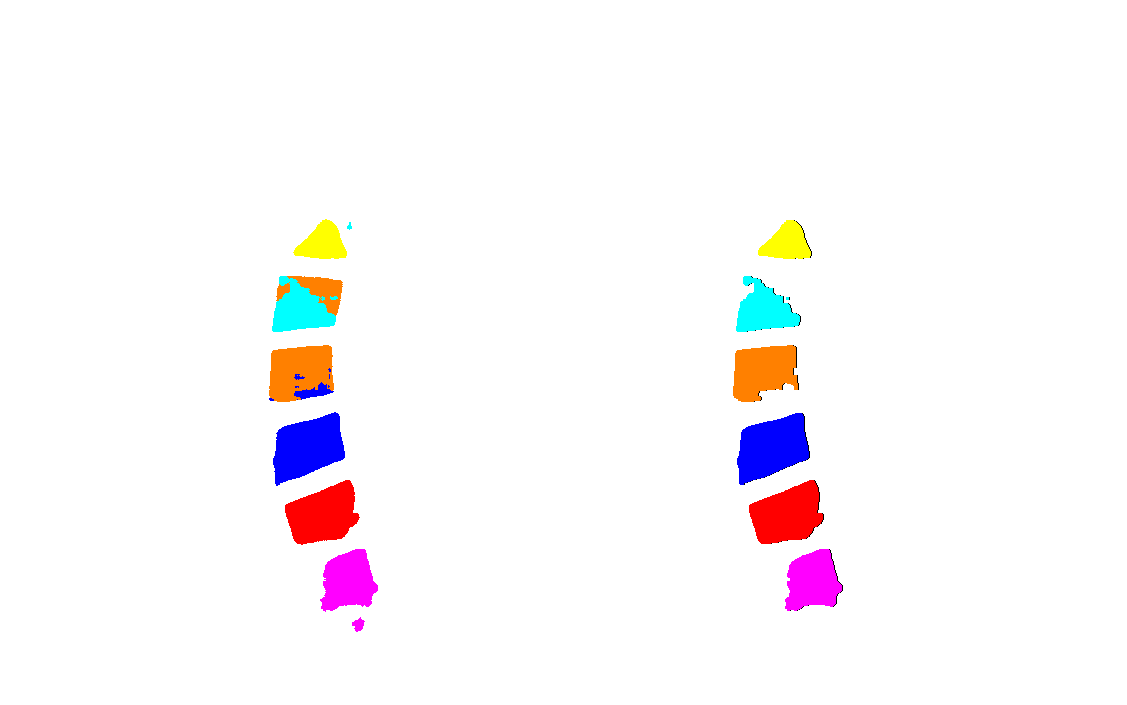
\includegraphics[width=0.6\linewidth]{images/postprocessing_showcase_whitebg.png}
    \caption{Ukázka postprocessingu segmentační masky (vlevo maska před a v pravo maska po postprocessingu). Pro ukázku byla zvolena maska s výraznými chybami pro lepší vizualizaci.}
    \label{fig:postprocessing}
\end{figure}


\section{Přímá detekce klíčových bodů}

Druhý zkoumaný přístup vychází z odlišné formulace úlohy než segmentační metoda popsaná v předchozí části. Zatímco u segmentačního přístupu je nejprve predikována maska jednotlivých obratlů a teprve následně jsou z této masky odvozovány referenční anatomické body, v přímém detekčním přístupu model předpovídá polohu klíčových bodů přímo z vstupního RTG snímku. Tím se celý problém redukuje na odhad omezeného počtu anatomicky významných klíčových bodů, z nichž lze následně dopočítat klinické metriky, jako je Cobbův úhel C2--C7, sagitální vertikální osa nebo segmentové úhly.

S ohledem na implementační náročnost modelů nebyl tento přístup v rámci této práce vyvíjen. Použitý model je vyvíjen Bc. Adélou Svítilovou v rámci její diplomové práce a v této práci je dále využit pro porovnání s navrženým segmentačním přístupem.

V použitém řešení je pro každý snímek detekováno celkem 23 klíčových bodů odpovídajících vybraným anatomickým strukturám obratlů C2 až C7. Konkrétně se jedná o body označené jako \texttt{bottom\_left}, \texttt{bottom\_right}, \texttt{top\_left}, \texttt{top\_right} a v případě obratle C2 také o centroid. Tyto body představují dostatečnou geometrickou reprezentaci pro výpočet sledovaných radiologických charakteristik.

Výhodou přímé detekce klíčových bodů je především jednodušší inferenční pipeline. Odpadá zde potřeba postprocessingu segmentačních masek, morfologického čištění i následné extrakce hran nebo centroidů z binárních oblastí. Model je optimalizován přímo na lokalizační úlohu, což může vést k přesnějšímu odhadu těch anatomických bodů, které jsou pro výpočet klinických metrik skutečně rozhodující. Nevýhodou naopak je, že model neposkytuje explicitní segmentační reprezentaci obratlů, a tudíž méně zachycuje tvarové informace o celé anatomické struktuře.

\subsection{Architektura detekčního modelu}

Pro přímou detekci klíčových bodů byl v této práci použit model typu \textbf{Stacked Hourglass} implementovaný v knihovně PyTorch. Architektura vychází z principu opakovaného zpracování obrazu ve více rozlišeních, kdy dochází ke střídání kroků snižování a následného obnovování prostorového rozlišení. Tím je možné současně zachytit globální kontext celého snímku i jemné lokální detaily potřebné pro přesnou lokalizaci anatomických klíčových bodů.

Použitá síť obsahuje vstupní konvoluční blok, na který navazují reziduální vrstvy a dvojice za sebou řazených hourglass modulů. V konfiguraci modelu je počet stacked bloků nastaven na $n = 2$, počet výstupních kanálů odpovídá počtu klíčových bodů, tedy 23, a model pracuje s RGB vstupem o velikosti $256 \times 256$ pixelů. Každý výstupní kanál reprezentuje jednu tepelnou mapu odpovídající jednomu anatomickému bodu.

Z hlediska zpracování obrazu lze architekturu rozdělit do tří částí:
\begin{enumerate}
    \item \textbf{Vstupní extrakce příznaků:} Na vstupní obraz je nejprve aplikována konvoluce se stride 2 a několik reziduálních bloků. Tato část redukuje prostorové rozlišení a současně vytváří bohatší příznakovou reprezentaci.
    \item \textbf{Hourglass moduly:} Každý hourglass blok obsahuje sestupnou větev s poolingem a reziduálními bloky, následovanou vzestupnou větví s upsamplingem. Díky tomu síť kombinuje lokální i globální informaci o poloze struktur v obraze.
    \item \textbf{Vícenásobná predikce:} Jelikož jde o stacked architekturu, výstup prvního hourglass modulu je využit nejen k vytvoření mezilehlé predikce, ale také jako vstup pro další hourglass blok. To umožňuje postupné zpřesňování odhadu polohy bodů.
\end{enumerate}

Výstup modelu má tvar:
\[
\mathbf{H} \in \mathbb{R}^{B \times N \times K \times 64 \times 64},
\]
kde $B$ značí velikost dávky, $N$ počet stacked modulů, $K = 23$ počet klíčových bodů a $64 \times 64$ rozlišení výstupních heatmap. Při vyhodnocení je pro další zpracování využívána poslední predikce v zásobníku, tedy poslední hourglass výstup, který reprezentuje finální odhad modelu.

Na rozdíl od segmentačního přístupu zde model nepředpovídá diskrétní třídy pixelů, ale spojité heatmapy s maximem v okolí správné polohy klíčového bodu. Tento způsob reprezentace je pro lokalizační úlohy výhodný, protože převádí odhad souřadnic na problém husté regresní predikce v obraze.

\begin{figure}[H]
    \centering
    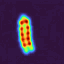
\includegraphics[width=0.5\linewidth]{images/heatmap.png}
    \caption{Výstupní heatmapa predikovaná modelem pro vstupní rentgenový snímek. Oblasti s vyšší intenzitou (teplejší) odpovídají místům s vyšší pravděpodobností výskytu hledaných klíčových bodů.}
    \label{fig:heatmap}
\end{figure}


\subsection{Reprezentace dat a trénování modelu}

Trénovací data jsou uložena ve formě tabulky, kde každému snímku odpovídá seznam souřadnic všech anotovaných klíčových bodů. Při načítání dat je původní RTG snímek převeden na formát \texttt{CHW}, normalizován do intervalu $\langle 0,1 \rangle$ a změněn na vstupní rozlišení $256 \times 256$ pixelů. Souřadnice anotovaných bodů jsou současně přepočteny do výstupního rozlišení $64 \times 64$, aby odpovídaly rozměrům predikovaných heatmap.

Pro každý klíčový bod je následně vytvořena referenční heatmapa pomocí dvourozměrného gaussovského rozložení se středem v anotované poloze. Pokud označíme souřadnice bodu jako $(k_x, k_y)$, pak hodnota referenční heatmapy v bodě $(x, y)$ je určena vztahem:
\begin{equation}
H(x,y) = \exp\left(-\frac{(x-k_x)^2 + (y-k_y)^2}{2\sigma^2}\right),
\end{equation}
kde v implementaci odpovídá parametr $\sigma$ hodnotě 2. Tím vzniká plynulý cíl, který je pro neuronovou síť vhodnější než přímá regrese diskrétních souřadnic.

Model je trénován pomocí optimalizačního algoritmu \texttt{Adam} s počáteční hodnotou learning rate $0{,}01$. Velikost dávky je nastavena na 8 a řízení learning rate je realizováno schedulerem \texttt{CosineAnnealingWarmRestarts} s parametry $T_0 = 4$, $T_{mult} = 2$ a $\eta_{\min} = 10^{-8}$. Tato strategie umožňuje periodické restartování procesu optimalizace a může přispět ke stabilnějšímu hledání minima ztrátové funkce.

Pro učení je v projektu použita vícestacková varianta Huberovy ztráty (\texttt{multi\_Huber}), která se počítá samostatně pro každý hourglass výstup a následně se přes všechny stacky průměruje. Tento postup motivuje síť, aby produkovala smysluplné heatmapy již v mezilehlých vrstvách, nejen v posledním výstupu. Trénování i validace probíhají nad heatmapovou reprezentací bodů, zatímco vyhodnocovací metriky pracují po převodu predikovaných heatmap zpět na souřadnice klíčových bodů.

Pro kvantitativní hodnocení byly použity dvě metriky:
\begin{itemize}
    \item \textbf{AED (Average Euclidean Distance)}, tedy průměrná eukleidovská vzdálenost mezi predikovanou a referenční polohou klíčových bodů,
    \item \textbf{PCK (Percentage of Correct Keypoints)}, která vyjadřuje podíl správně lokalizovaných bodů při zvolené toleranci. V implementaci je bod považován za správně určený tehdy, pokud jeho vzdálenost od reference nepřesáhne $0{,}5$ násobku normalizačního koeficientu, tj. referenční délky použité k převedení toleranční meze na relativní měřítko nezávislé na velikosti obrazu.
\end{itemize}

\subsection{Inference a převod heatmap na souřadnice}

Při inferenci je z načteného checkpointu obnovena naučená váha modelu a síť je přepnuta do evaluačního režimu. Vstupní snímky jsou zpracovávány po dávkách a pro každý snímek vzniká sada 23 heatmap. Z finálního stacku modelu je pro každý klíčový bod určena poloha maxima, tedy pixel s nejvyšší hodnotou v odpovídající heatmapě. Formálně lze predikovanou polohu $i$-tého bodu vyjádřit jako:
\begin{equation}
(\hat{x}_i, \hat{y}_i) = \arg\max_{x,y} H_i(x,y),
\end{equation}
kde $H_i$ značí predikovanou heatmapu příslušného bodu.

Tento krok představuje základní postprocessing detekčního modelu. Ve srovnání se segmentačním přístupem je výrazně jednodušší, protože nevyžaduje morfologické operace ani analýzu souvislých komponent. Výsledkem inference je přímo seznam souřadnic klíčových bodů, který lze uložit například ve formátu JSON nebo CSV a dále použít pro výpočet klinických metrik.

Je však třeba upozornit, že predikované souřadnice jsou v této podobě určeny v rozlišení výstupních heatmap, tedy v mřížce $64 \times 64$. Při výpočtu klinických charakteristik v původním měřítku snímku je proto nutné zajistit odpovídající zpětný přepočet do rozlišení originálního obrazu. Přesnost výsledných metrik tak nezávisí pouze na samotné kvalitě detekce bodů, ale také na korektním mapování mezi vstupním obrazem, heatmapou a původním souřadnicovým systémem snímku.

Volba rozlišení heatmap představuje důležitý kompromis mezi lokalizační přesností a výpočetní náročností. Pokud by byly použity heatmapy s vyšším rozlišením než $64 \times 64$, bylo by možné jemněji reprezentovat polohu maxima a snížit kvantizační chybu při převodu do souřadnic původního obrazu. To by mohlo být výhodné zejména v případech, kdy i malý posun bodu vede k citelné změně výsledné klinické metriky, například u výpočtu úhlů nebo vzdáleností mezi obratli.

Vyšší rozlišení heatmap však současně zvyšuje paměťové nároky modelu, množství výpočetních operací i dobu inference. Zároveň nelze předpokládat, že samotné zvětšení heatmap automaticky povede k lepší přesnosti, protože výsledná kvalita lokalizace závisí také na schopnosti modelu naučit se dostatečně diskriminační prostorové reprezentace. V praxi je proto rozlišení $64 \times 64$ často voleno jako rozumný kompromis mezi výpočetní efektivitou a přesností lokalizace. Další zvýšení rozlišení by bylo vhodné ověřit experimentálně, protože jeho přínos by se mohl projevit jen u některých bodů nebo pouze při současné úpravě architektury modelu a způsobu dekódování souřadnic.


\chapter{Výsledky}

Tato kapitola prezentuje výsledky experimentální části práce se zaměřením na porovnání segmentačního přístupu a přístupu založeného na detekci klíčových bodů. Vyhodnocení bylo provedeno na úrovni klinických metrik odvozených z predikovaných anatomických bodů, nikoli pouze na úrovni pixelové nebo bodové přesnosti. Hlavním cílem kapitoly je ukázat, s jakou přesností byly jednotlivé metriky určeny a který z obou přístupů poskytl přesnější výstupy vzhledem k zadání práce.

Pro každý snímek a každou metriku byla k dispozici referenční hodnota (\texttt{gt}), predikovaná hodnota (\texttt{pred}) a jejich rozdíl (\texttt{delta}). Kvantitativně byly hodnoceny metriky Cobbův úhel C2--C7, sklon C2, sagitální osa C2--C7 a segmentové úhly mezi sousedními obratli. Jacksonův úhel C2--C7 nebyl do výsledkové části zařazen, protože použitý dataset neobsahuje horní rohy obratle C2 ani jinou přímou anotaci zadní horní hrany C2, a metriku tak nebylo možné korektně spočítat bez dodatečného odhadu. Přesnost hodnocených metrik byla vyjádřena pomocí průměrné absolutní chyby (MAE), odmocniny střední kvadratické chyby (RMSE), směrodatné odchylky chyby a Pearsonova korelačního koeficientu.

\section{Sjednocení evaluační množiny}

Původní dataset obsahoval celkem 4\,963 snímků. Při samostatném vyhodnocení však nebyly oba přístupy vyhodnoceny nad totožnou množinou případů. U segmentačního přístupu bylo do souhrnných výsledků zařazeno 4\,955 snímků, zatímco u přístupu založeného na detekci klíčových bodů 4\,962 snímků.

Rozdíl v počtu vyhodnocených případů měl dva důvody. U segmentačního přístupu bylo 8 snímků vyřazeno při výpočtu klinických metrik z důvodu chybějícího bodu \texttt{C7 bottom left}, který je potřebný pro výpočet části sledovaných charakteristik. U detekčního přístupu naopak chyběl již ve vstupních predikcích 1 snímek. Pro přímé srovnání obou metod proto byla použita sjednocená evaluační množina tvořená průnikem obou množin, která obsahovala 4\,954 snímků.

Protože však není vhodné společně prezentovat výsledky na trénovacích i testovacích datech, byla tato sjednocená množina dále rozdělena podle rozdělení pro fold 0, na němž byly oba modely trénovány. Trénovací část tak obsahovala 3\,963 snímků a testovací část 991 snímků. Veškeré hlavní závěry v této kapitole jsou proto formulovány na základě testovací části sjednocené evaluační množiny. Výsledky na trénovací části jsou uváděny pouze doplňkově, zejména pro posouzení stability obou přístupů a rozdílu mezi oběma částmi dat.

\section{Srovnání podle jednotlivých metrik}

Podrobné srovnání obou přístupů pro jednotlivé klinické metriky na testovací části sjednocené evaluační množiny je uvedeno v tabulce~\ref{tab:metric_comparison}. Segmentační přístup dosáhl nižší MAE, nižší RMSE a vyšší Pearsonovy korelace u všech osmi hodnocených metrik. Nejmenší absolutní chyba byla u segmentačního modelu zaznamenána u sagitální osy C2--C7 a u sklonu C2. U detekčního přístupu byly nejvyšší chyby pozorovány u Cobbova úhlu C2--C7 a u segmentových úhlů.

\begin{table}[htbp]
\centering
\small
\caption{Srovnání přesnosti obou přístupů podle jednotlivých klinických metrik na testovací části sjednocené evaluační množiny.}
\label{tab:metric_comparison}
\begin{tabular}{p{3.3cm}rrrrrr}
\hline
Metrika & MAE seg. & MAE det. & RMSE seg. & RMSE det. & $r$ seg. & $r$ det. \\
\hline
Cobb. C2--C7 ($^\circ$) & 2.568 & 7.031 & 4.274 & 8.783 & 0.941 & 0.763 \\
SVA C2--C7 (px) & 1.627 & 3.643 & 3.198 & 4.583 & 0.995 & 0.989 \\
Seg. úhel C2--C3 ($^\circ$) & 2.176 & 6.126 & 3.076 & 7.879 & 0.791 & 0.265 \\
Seg. úhel C3--C4 ($^\circ$) & 1.898 & 6.246 & 2.458 & 7.993 & 0.870 & 0.428 \\
Seg. úhel C4--C5 ($^\circ$) & 1.873 & 6.329 & 2.464 & 7.975 & 0.887 & 0.392 \\
Seg. úhel C5--C6 ($^\circ$) & 1.897 & 6.204 & 2.515 & 7.776 & 0.880 & 0.435 \\
Seg. úhel C6--C7 ($^\circ$) & 2.473 & 6.400 & 4.677 & 7.917 & 0.600 & 0.267 \\
Sklon C2 ($^\circ$) & 1.695 & 4.963 & 2.564 & 6.278 & 0.958 & 0.753 \\
\hline
\end{tabular}
\normalsize
\end{table}

\begin{table}[htbp]
\centering
\small
\caption{Srovnání přesnosti obou přístupů podle jednotlivých klinických metrik na trénovací části sjednocené evaluační množiny.}
\label{tab:metric_comparison_train}
\begin{tabular}{p{3.3cm}rrrrrr}
\hline
Metrika & MAE seg. & MAE det. & RMSE seg. & RMSE det. & $r$ seg. & $r$ det. \\
\hline
Cobb. C2--C7 ($^\circ$) & 2.091 & 6.814 & 2.664 & 8.558 & 0.977 & 0.785 \\
SVA C2--C7 (px) & 1.179 & 3.495 & 1.505 & 4.333 & 0.999 & 0.990 \\
Seg. úhel C2--C3 ($^\circ$) & 1.893 & 6.531 & 2.405 & 8.319 & 0.879 & 0.307 \\
Seg. úhel C3--C4 ($^\circ$) & 1.795 & 6.319 & 2.291 & 7.965 & 0.898 & 0.430 \\
Seg. úhel C4--C5 ($^\circ$) & 1.743 & 6.256 & 2.267 & 7.894 & 0.903 & 0.427 \\
Seg. úhel C5--C6 ($^\circ$) & 1.742 & 6.058 & 2.257 & 7.671 & 0.897 & 0.395 \\
Seg. úhel C6--C7 ($^\circ$) & 2.083 & 6.294 & 2.701 & 7.812 & 0.829 & 0.271 \\
Sklon C2 ($^\circ$) & 1.334 & 5.154 & 1.709 & 6.359 & 0.981 & 0.756 \\
\hline
\end{tabular}
\normalsize
\end{table}


Tabulky~\ref{tab:metric_comparison} a \ref{tab:metric_comparison_train} ukazují, že segmentační přístup vykazoval nejlepší výsledky zejména u globálních metrik. U sagitální osy C2--C7 dosáhl na testovací části MAE 1{,}627~px a Pearsonova korelačního koeficientu 0{,}995, zatímco detekční přístup dosáhl MAE 3{,}643~px a korelace 0{,}989. Podobně u sklonu C2 dosáhla segmentace MAE 1{,}695$^\circ$, zatímco keypoint detection 4{,}963$^\circ$.

Výrazný rozdíl byl patrný také u Cobbova úhlu C2--C7, kde segmentační model dosáhl MAE 2{,}568$^\circ$ a Pearsonova koeficientu 0{,}941, zatímco detekční přístup vykázal MAE 7{,}031$^\circ$ a korelaci 0{,}763. U segmentových úhlů byly rozdíly mezi oběma přístupy ještě výraznější. Zatímco u segmentačního modelu se MAE na testovací části pohybovala přibližně mezi 1{,}87$^\circ$ a 2{,}47$^\circ$, u keypoint detection se pohybovala mezi 6{,}13$^\circ$ a 6{,}40$^\circ$.

\begin{figure}[H]
    \centering
    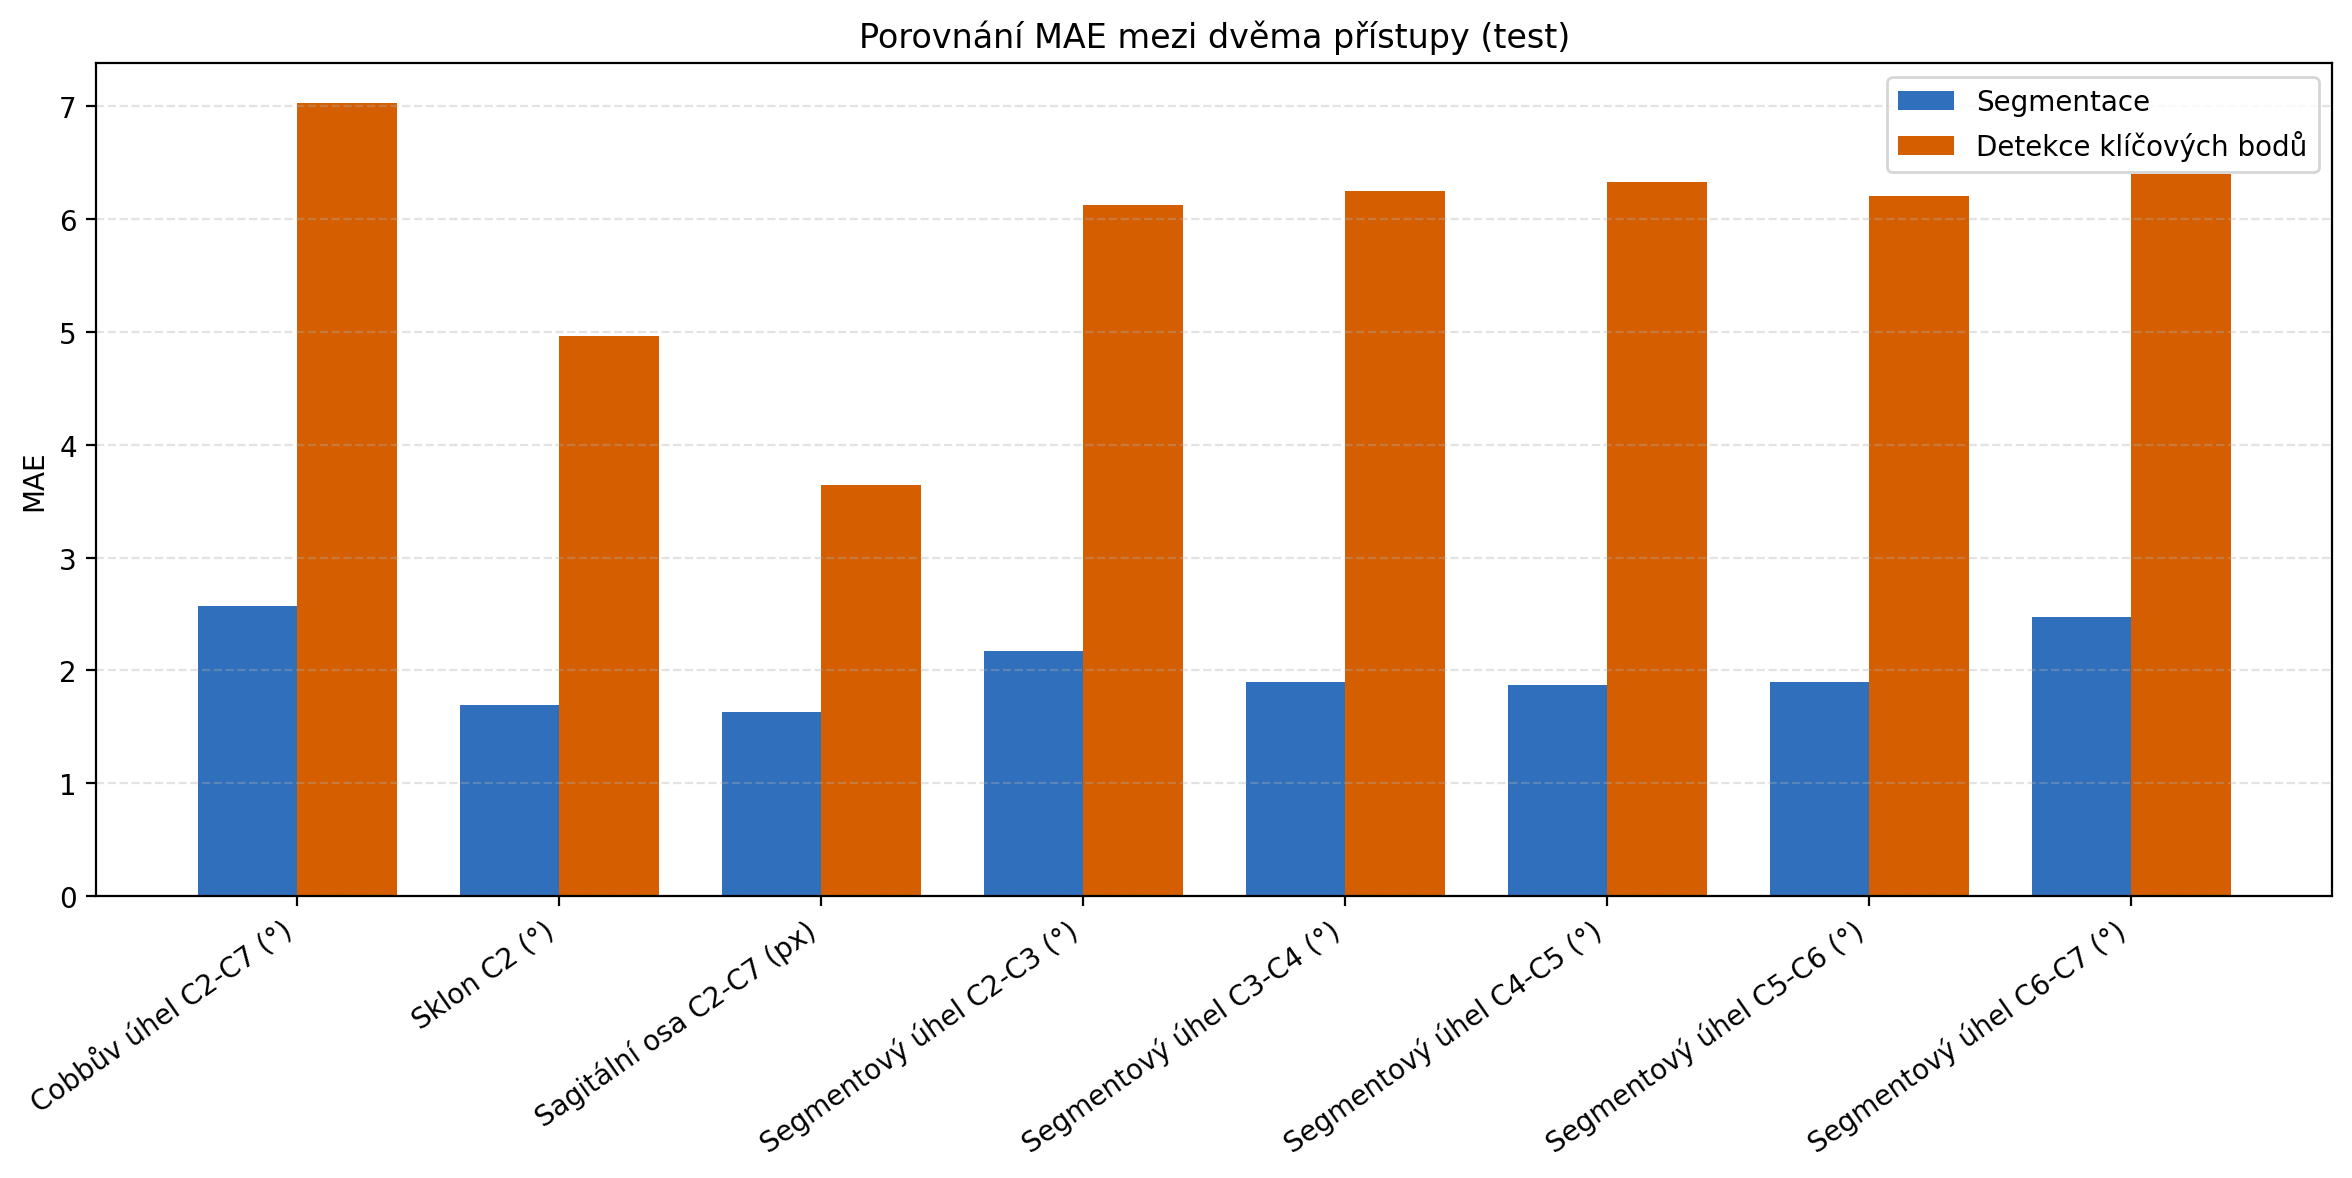
\includegraphics[width=0.95\linewidth]{images/results/test/mae_bar_comparison.png}
    \caption{Srovnání průměrné absolutní chyby jednotlivých klinických metrik mezi segmentačním a detekčním přístupem na testovacích datech. Pro úhly se jedná o chybu ve stupních a u vzdáleností v pixelech.}
    \label{fig:mae_comparison_test}
\end{figure}

\begin{figure}[H]
    \centering
    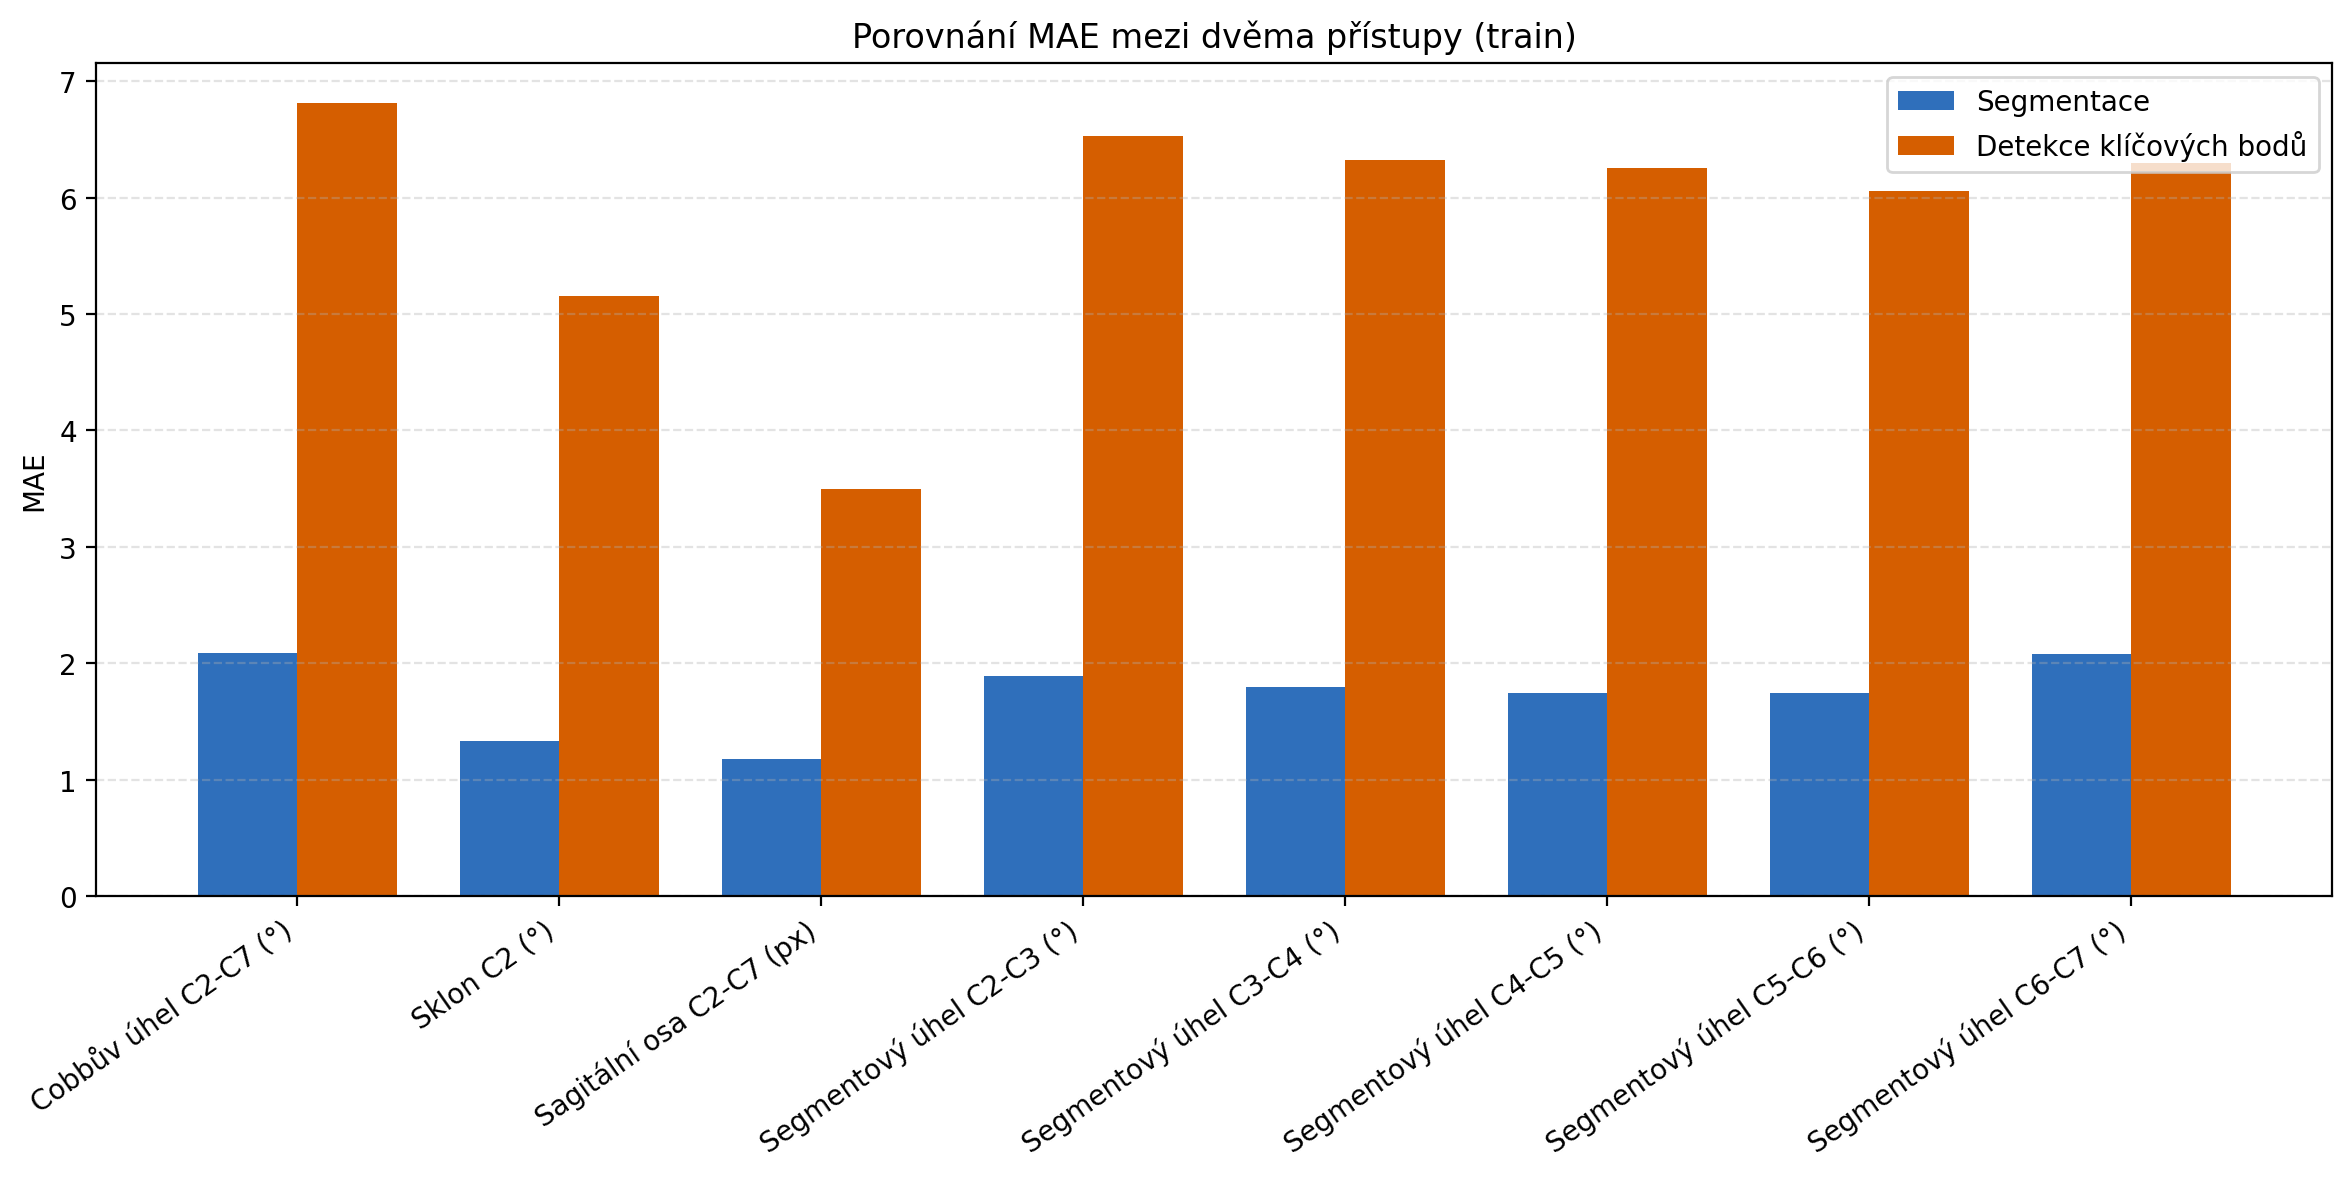
\includegraphics[width=0.95\linewidth]{images/results/train/mae_bar_comparison.png}
    \caption{Srovnání průměrné absolutní chyby jednotlivých klinických metrik mezi segmentačním a detekčním přístupem na trénovacích datech. Pro úhly se jedná o chybu ve stupních a u vzdáleností v pixelech.}
    \label{fig:mae_comparison_train}
\end{figure}

Grafy na obrázcích~\ref{fig:mae_comparison_test} a~\ref{fig:mae_comparison_train} současně ukazují, že pořadí obou přístupů zůstává stejné i na trénovací části dat. U segmentačního přístupu jsou však na testovací části patrné vyšší chyby zejména u Cobbova úhlu C2--C7, SVA C2--C7 a segmentového úhlu C6--C7. U detekčního přístupu jsou rozdíly mezi oběma částmi dat menší, což je v souladu i se souhrnnými výsledky z tabulky~\ref{tab:overall_comparison}.

\section{Výsledky hlavních klinických metrik}

\subsection{Cobbův úhel C2--C7}

U Cobbova úhlu C2--C7 byla i na testovací části zjištěna výrazně vyšší shoda mezi referenčními a predikovanými hodnotami u segmentačního přístupu. MAE dosáhla 2{,}568$^\circ$, RMSE činila 4{,}274$^\circ$ a Pearsonův korelační koeficient byl 0{,}941. U keypoint detection byla chyba vyšší, konkrétně MAE 7{,}031$^\circ$ a RMSE 8{,}783$^\circ$, přičemž korelace klesla na 0{,}763.

Ve srovnání s trénovací částí se u segmentačního modelu projevilo zhoršení z MAE 2{,}091$^\circ$ na 2{,}568$^\circ$, zatímco u detekčního přístupu se hodnota změnila pouze z 6{,}814$^\circ$ na 7{,}031$^\circ$. Segmentační přístup tak zůstal přesnější i po přechodu na neviděná data, přestože právě u Cobbova úhlu byl rozdíl mezi trénovací a testovací částí jedním z nejvýraznějších.

V bodovém grafu detekce klíčových bodů (obrázek \ref{fig:scatter_det_test_cobb_c2_c7}) je patrné, že se body u seskupují do několika podobných úrovní. Tento jev je způsoben převodem výstupu detekčního modelu z heatmapy na konkrétní souřadnice klíčových bodů. Protože heatmapa má omezené prostorové rozlišení, výsledné predikované body mohou nabývat pouze určitých diskrétních poloh, což se následně projeví i ve vypočtených klinických metrikách. Tento jev můžeme pozorovat i u dalších metrik (obrázky \ref{fig:scatter_det_test_sva_c2_c7} a \ref{fig:scatter_det_test_slope_c2})

\begin{figure}[H]
    \centering
    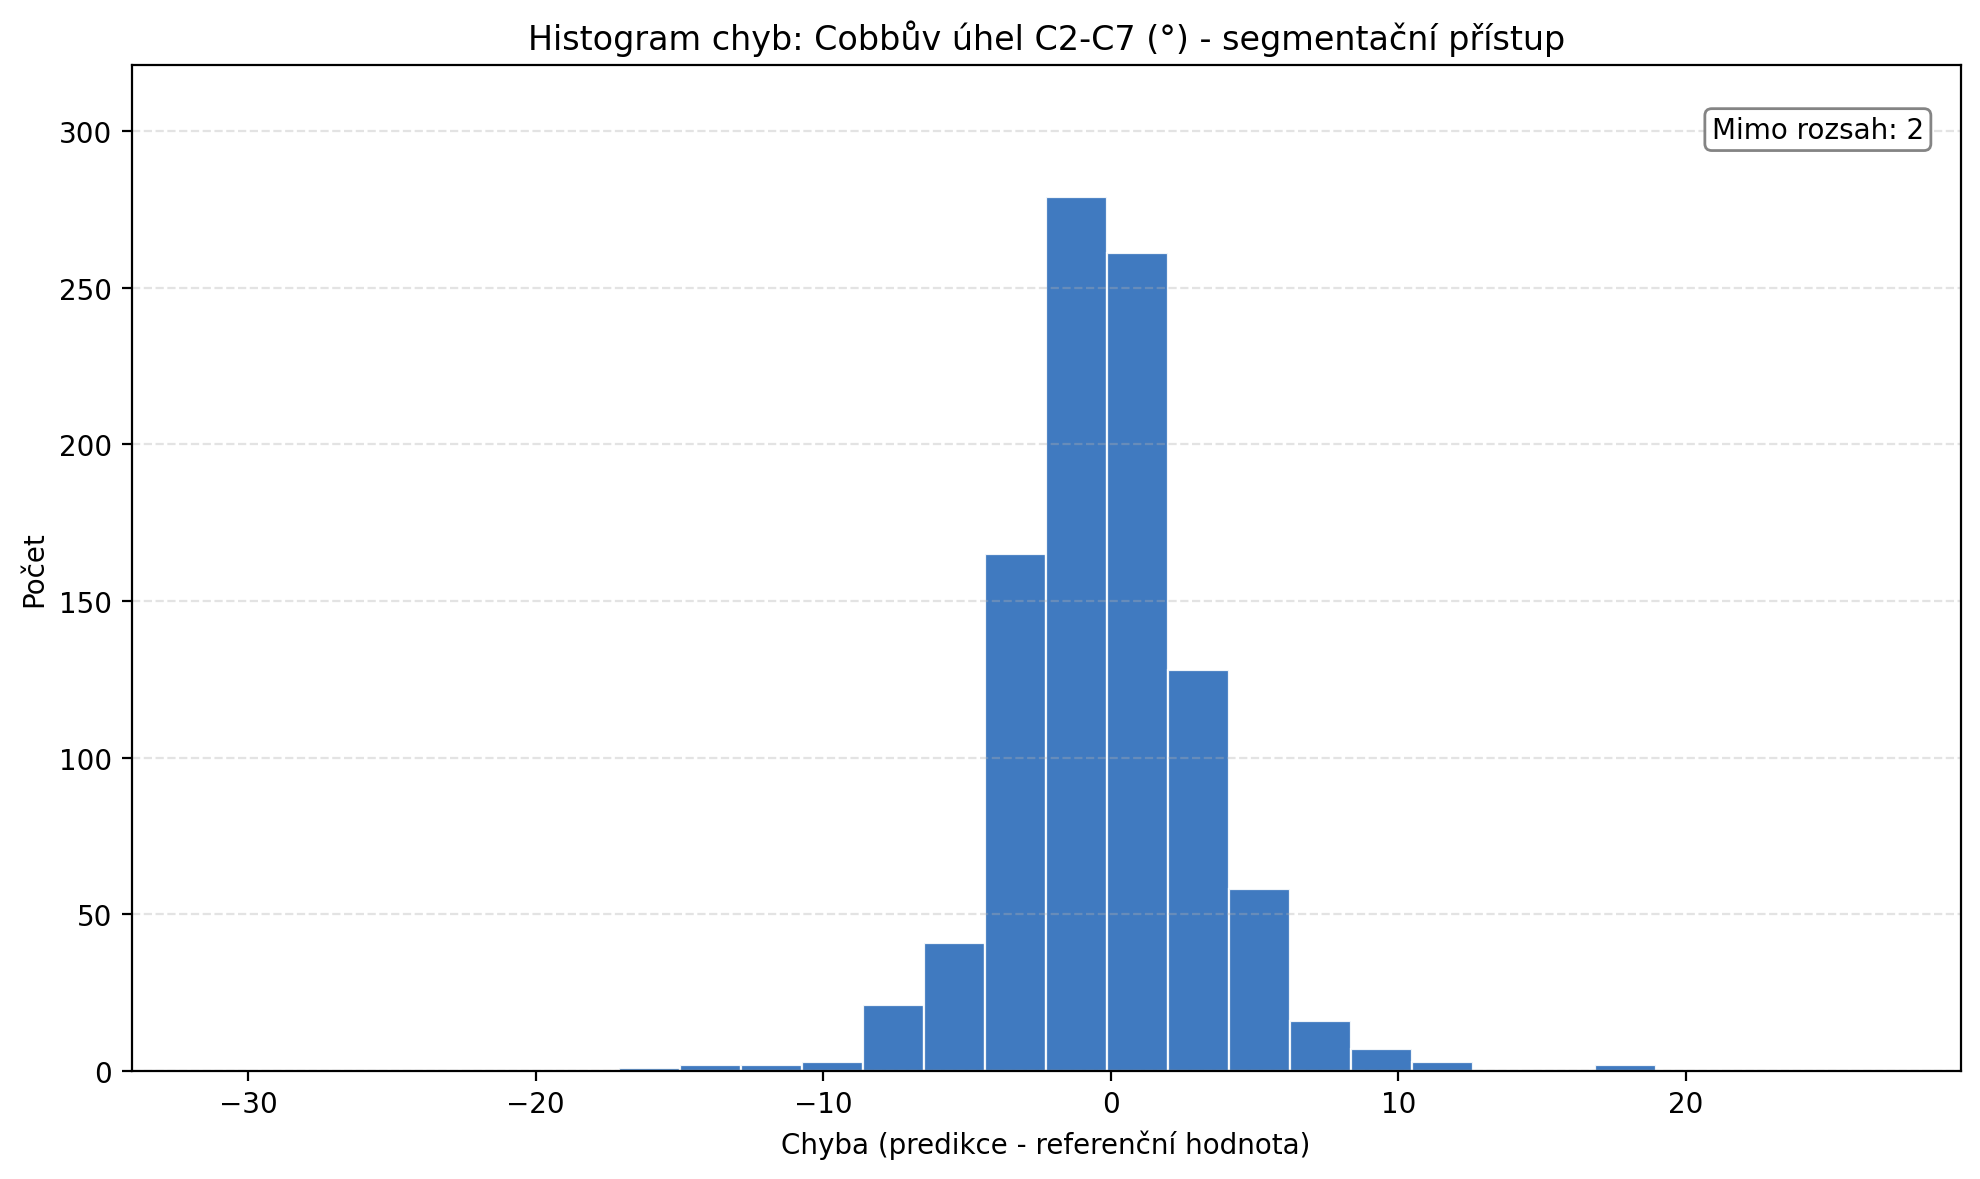
\includegraphics[width=0.75\linewidth]{images/results/test/seg/hist/Cobb_C2_C7_deg_error_histogram.png}
    \caption{Histogram chyb výpočtu Cobbova úhlu C2--C7 u segmentačního přístupu na testovací množině. Chyba je definována jako rozdíl mezi predikovanou a referenční hodnotou.}
    \label{fig:hist_seg_test_cobb_c2_c7}
\end{figure}

\begin{figure}[H]
    \centering
    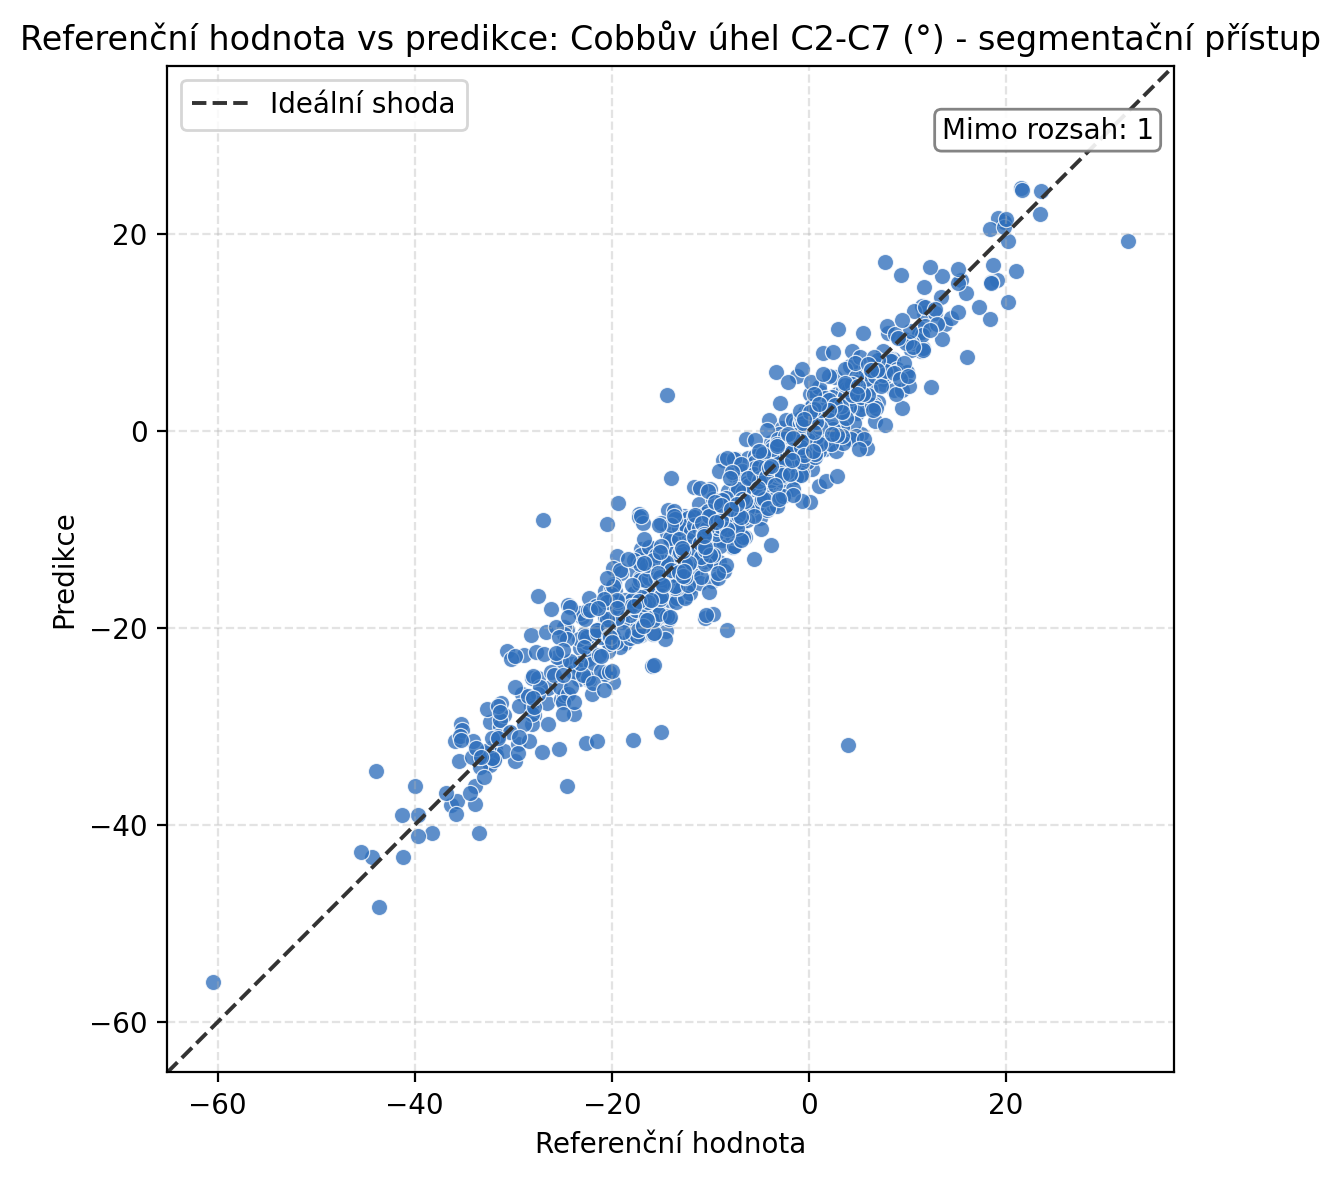
\includegraphics[width=0.75\linewidth]{images/results/test/seg/scatter/Cobb_C2_C7_deg_scatter_gt_vs_pred.png}
    \caption{Porovnání referenčních a predikovaných hodnot Cobbova úhlu C2--C7 u segmentačního přístupu na testovací množině. Přerušovaná přímka znázorňuje ideální shodu predikce s referencí.}
    \label{fig:scatter_seg_test_cobb_c2_c7}
\end{figure}

\begin{figure}[H]
    \centering
    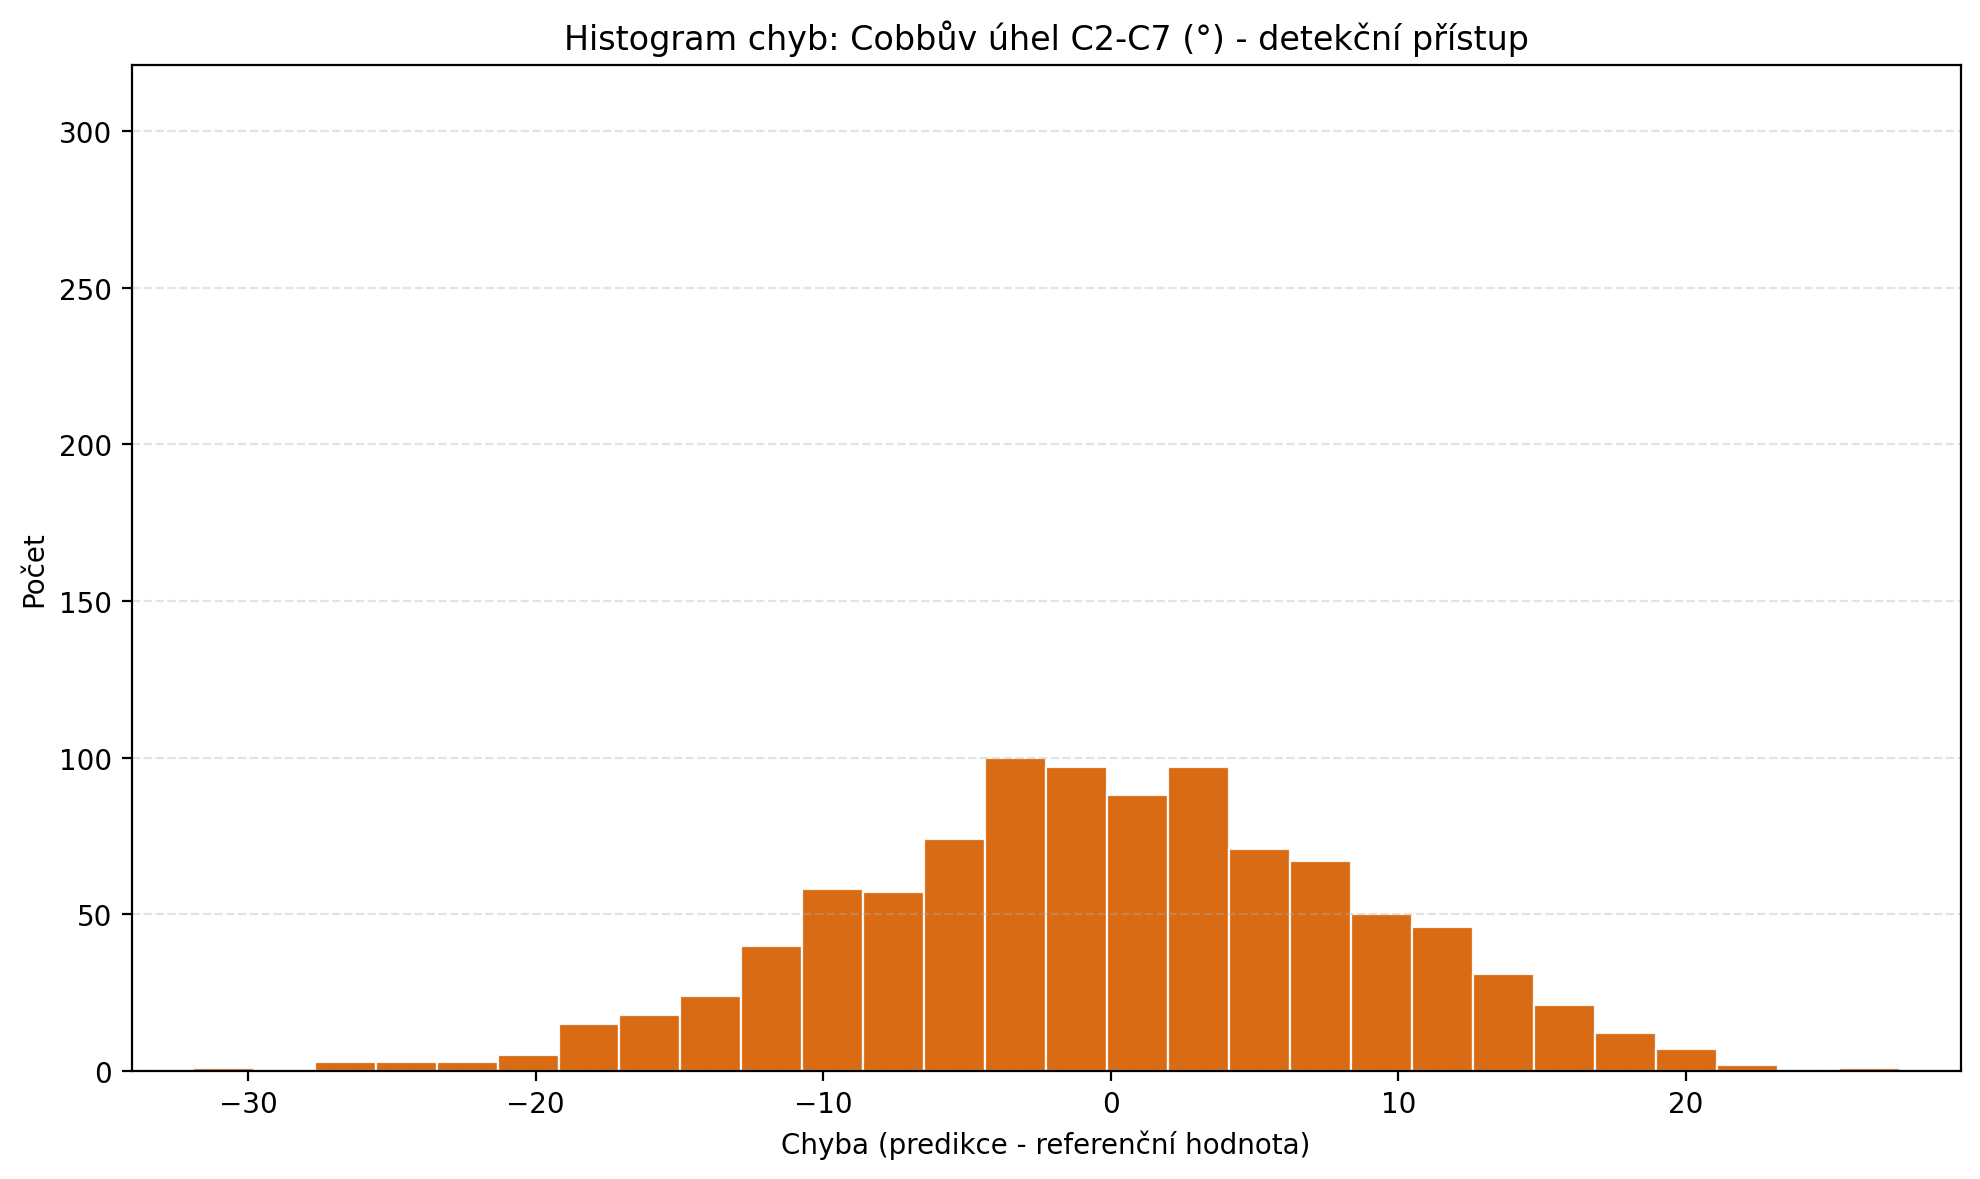
\includegraphics[width=0.75\linewidth]{images/results/test/det/hist/Cobb_C2_C7_deg_error_histogram.png}
    \caption{Histogram chyb výpočtu Cobbova úhlu C2--C7 u detekčního přístupu na testovací množině. Chyba je definována jako rozdíl mezi predikovanou a referenční hodnotou.}
    \label{fig:hist_det_test_cobb_c2_c7}
\end{figure}

\begin{figure}[H]
    \centering
    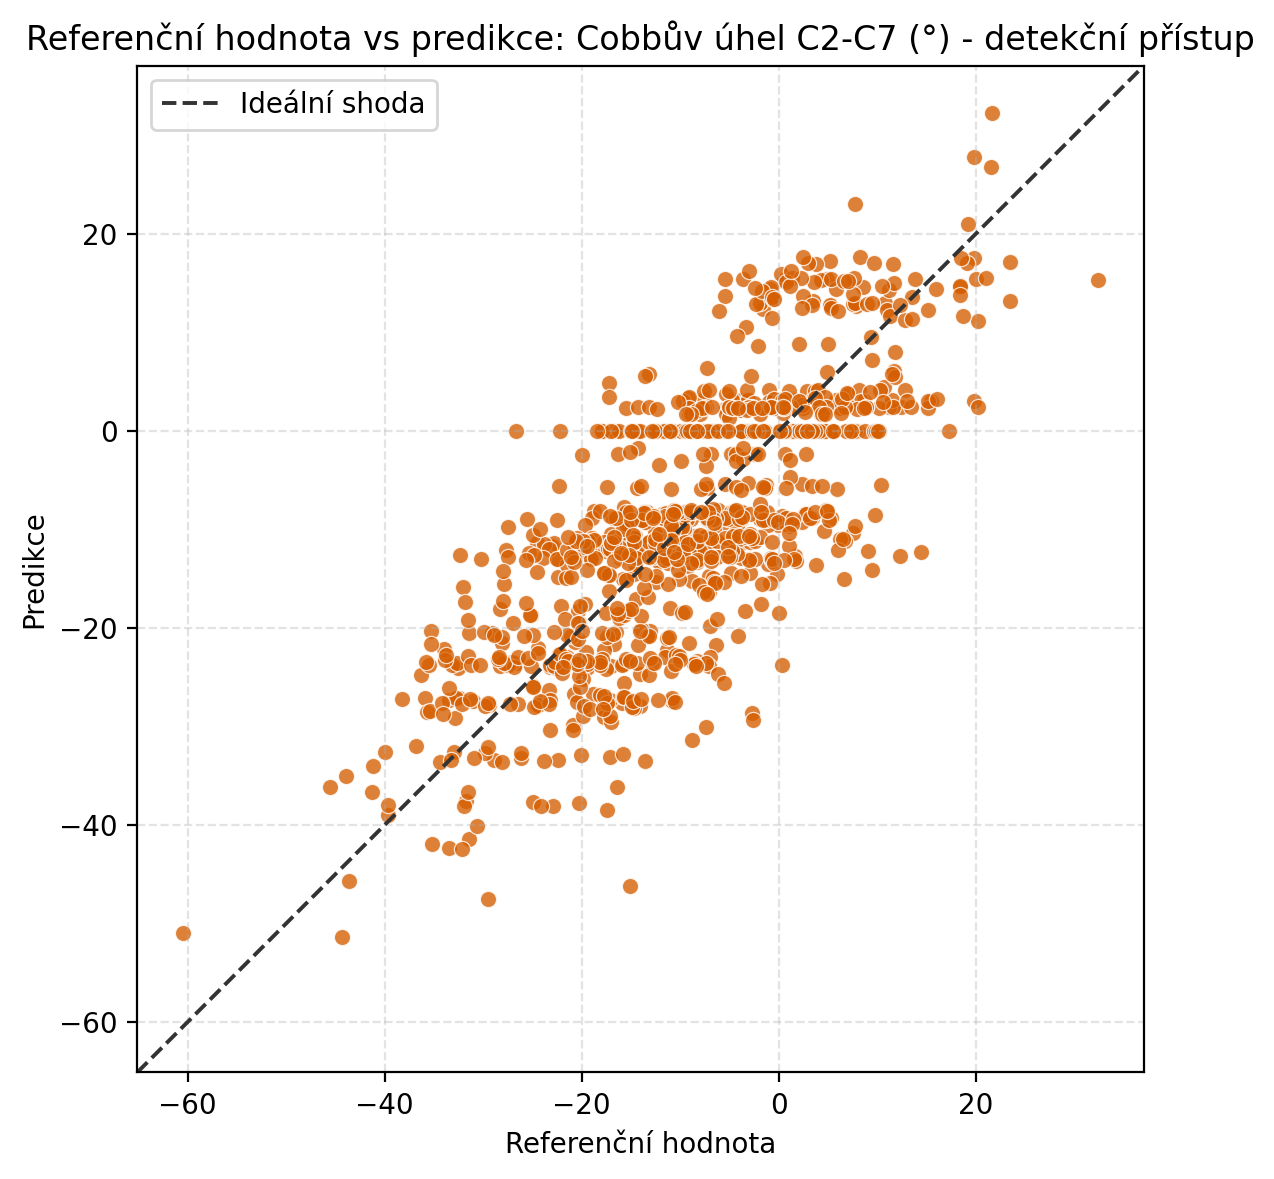
\includegraphics[width=0.75\linewidth]{images/results/test/det/scatter/Cobb_C2_C7_deg_scatter_gt_vs_pred.png}
    \caption{Porovnání referenčních a predikovaných hodnot Cobbova úhlu C2--C7 u detekčního přístupu na testovací množině. Přerušovaná přímka znázorňuje ideální shodu predikce s referencí.}
    \label{fig:scatter_det_test_cobb_c2_c7}
\end{figure}

\subsection{Sagitální osa C2--C7}

Sagitální osa C2--C7 představovala metriku s nejvyšší dosaženou shodou u obou přístupů i na testovací části. Segmentační model dosáhl MAE 1{,}627~px, RMSE 3{,}198~px a Pearsonova korelačního koeficientu 0{,}995. Keypoint detection dosáhla MAE 3{,}643~px, RMSE 4{,}583~px a Pearsonova koeficientu 0{,}989.

Přestože i detekční přístup vykázal u této metriky vysokou korelaci, segmentační model dosáhl nižší absolutní chyby i menšího rozptylu odchylek. Na trénovací části byly navíc chyby obou přístupů mírně nižší, zejména u segmentace, která zde dosáhla MAE 1{,}179~px. Sagitální osa C2--C7 tak byla nejpřesněji určovanou metrikou v celé studii.

\begin{figure}[H]
    \centering
    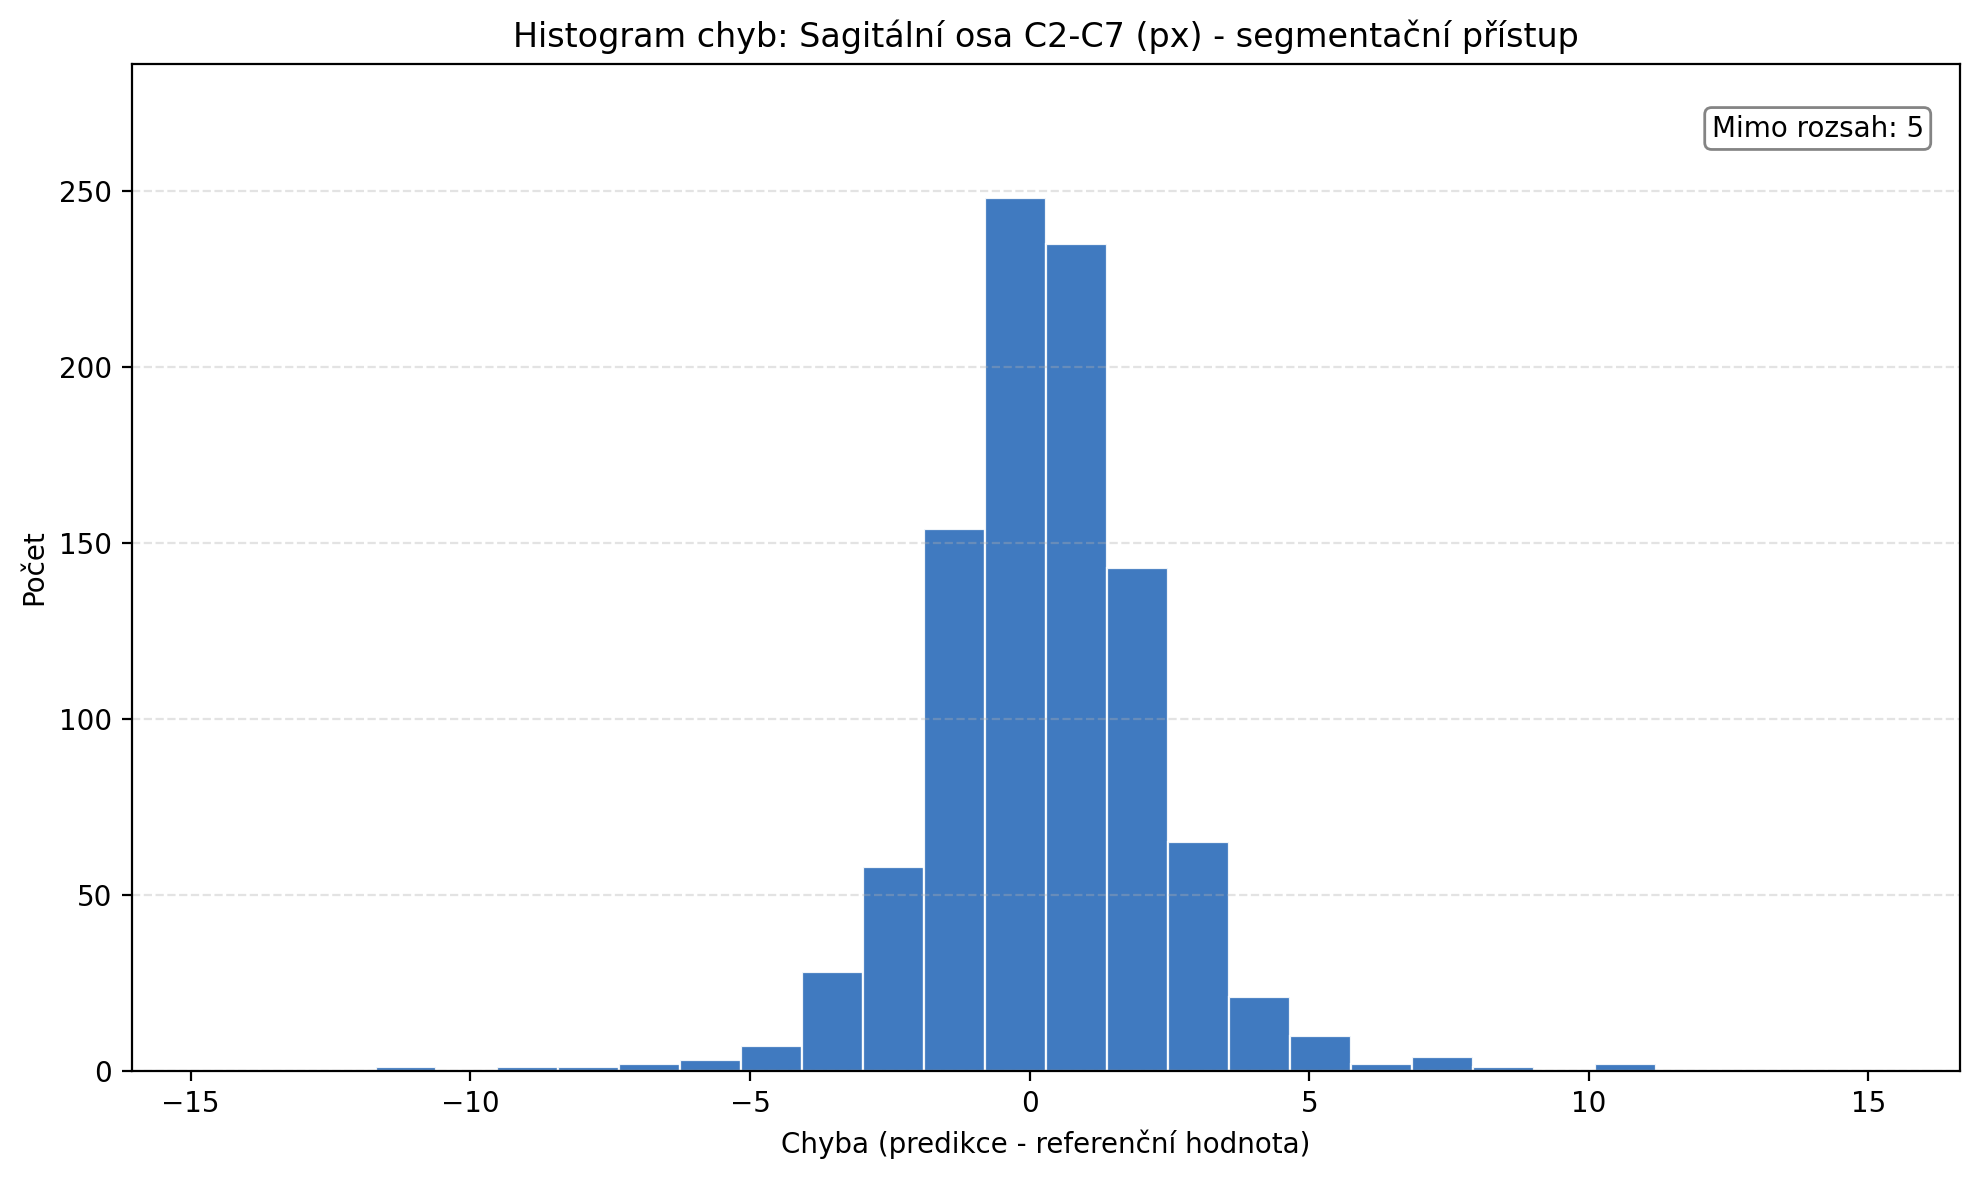
\includegraphics[width=0.75\linewidth]{images/results/test/seg/hist/SVA_C2_C7_px_error_histogram.png}
    \caption{Histogram chyb výpočtu sagitální vertikální osy C2--C7 u segmentačního přístupu na testovací množině. Chyba je definována jako rozdíl mezi predikovanou a referenční hodnotou.}
    \label{fig:hist_seg_test_sva_c2_c7}
\end{figure}

\begin{figure}[H]
    \centering
    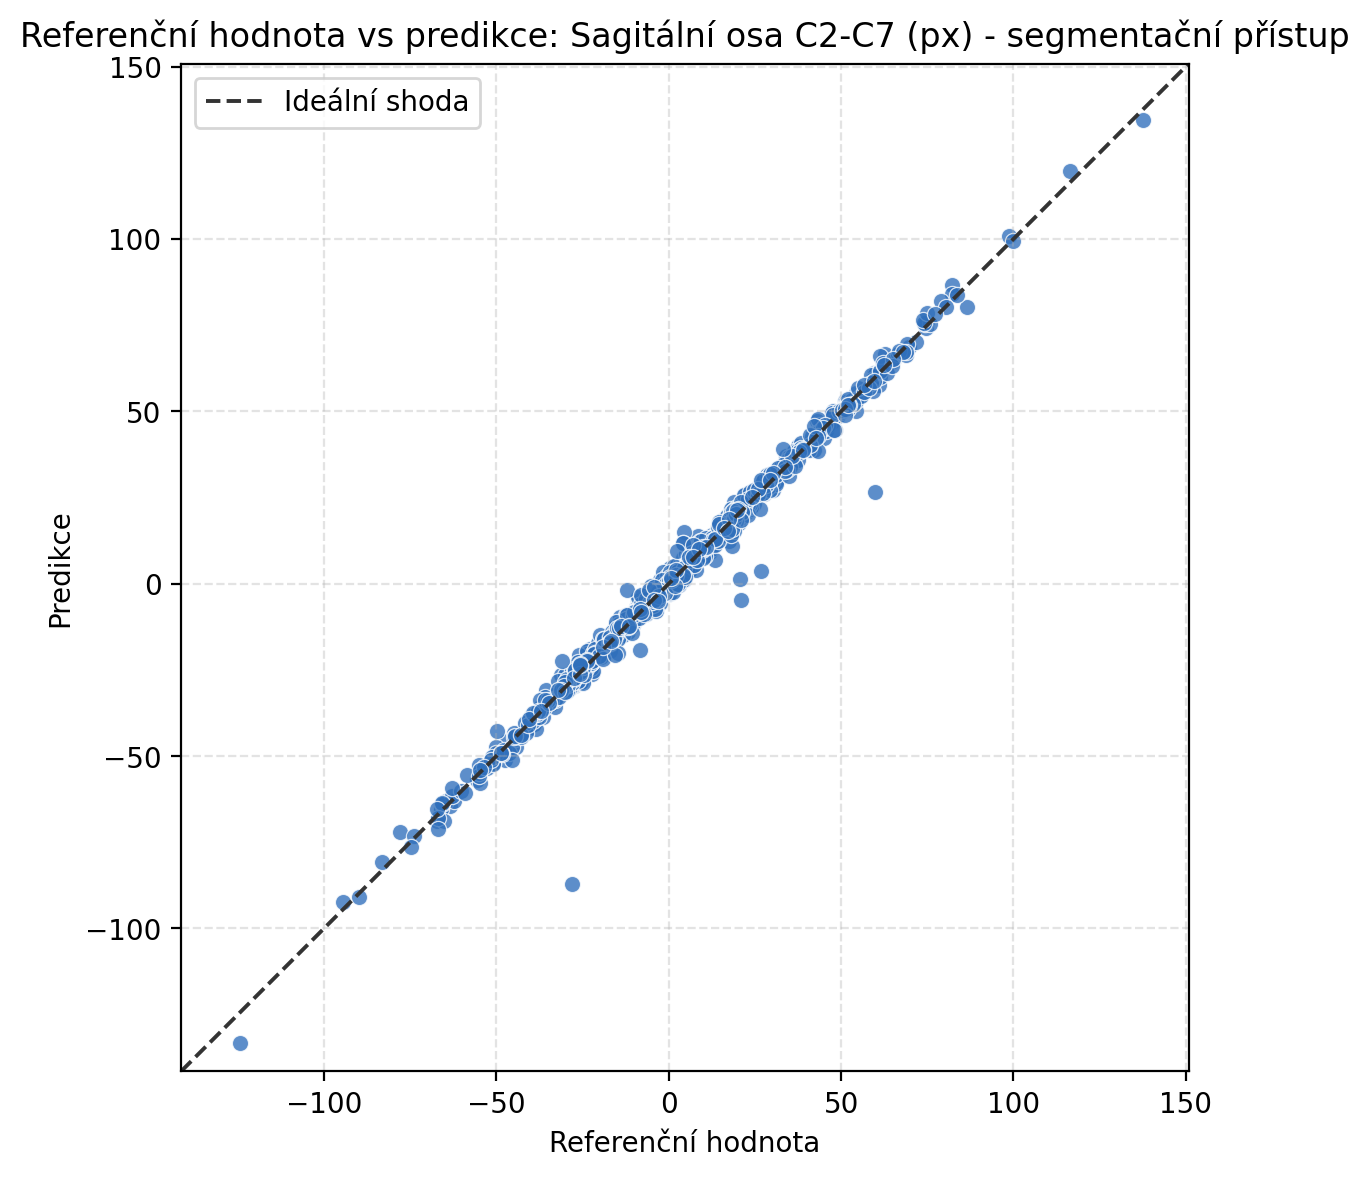
\includegraphics[width=0.75\linewidth]{images/results/test/seg/scatter/SVA_C2_C7_px_scatter_gt_vs_pred.png}
    \caption{Porovnání referenčních a predikovaných hodnot sagitální vertikální osy C2--C7 u segmentačního přístupu na testovací množině. Přerušovaná přímka znázorňuje ideální shodu predikce s referencí.}
    \label{fig:scatter_seg_test_sva_c2_c7}
\end{figure}

\begin{figure}[H]
    \centering
    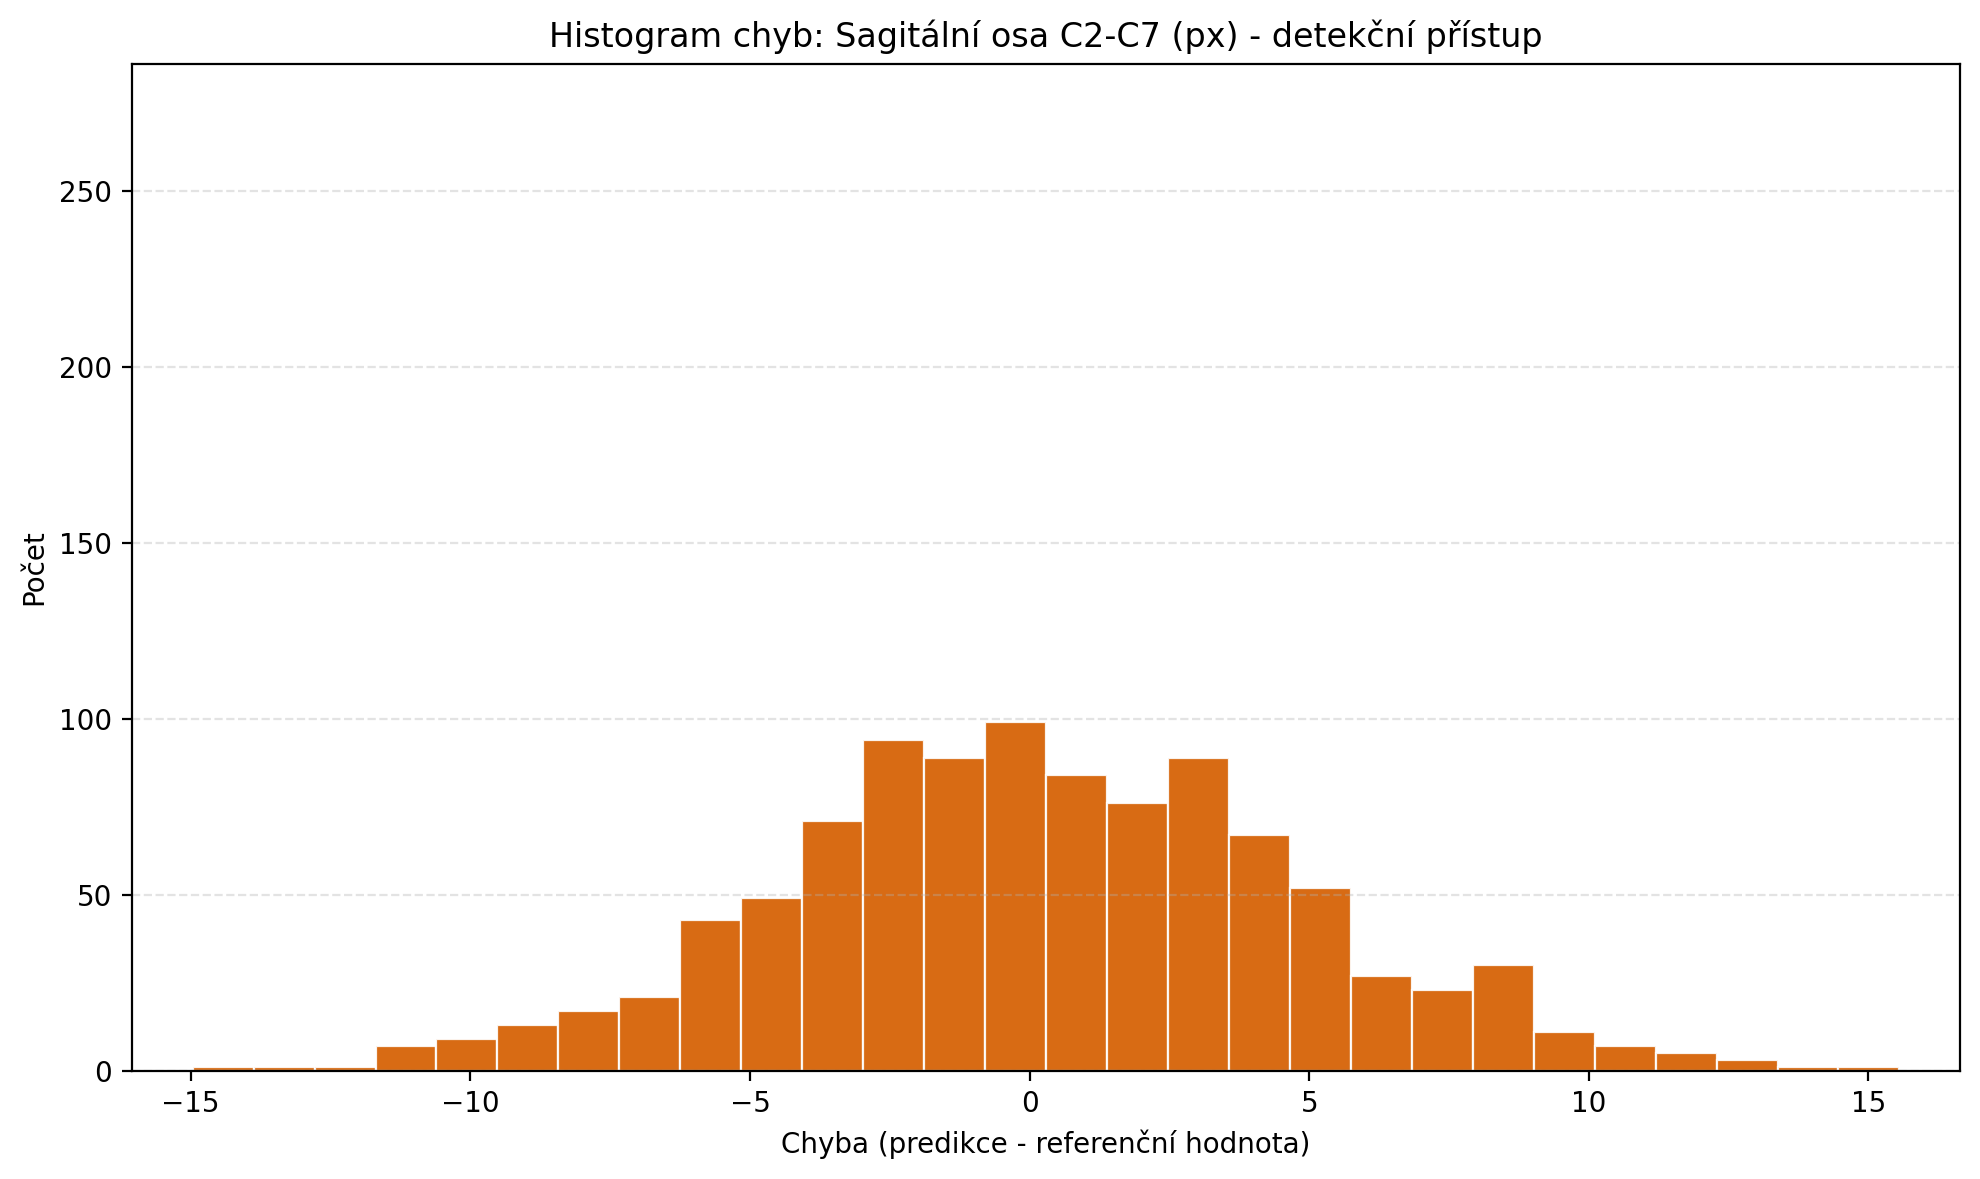
\includegraphics[width=0.75\linewidth]{images/results/test/det/hist/SVA_C2_C7_px_error_histogram.png}
    \caption{Histogram chyb výpočtu sagitální vertikální osy C2--C7 u detekčního přístupu na testovací množině. Chyba je definována jako rozdíl mezi predikovanou a referenční hodnotou.}
    \label{fig:hist_det_test_sva_c2_c7}
\end{figure}

\begin{figure}[H]
    \centering
    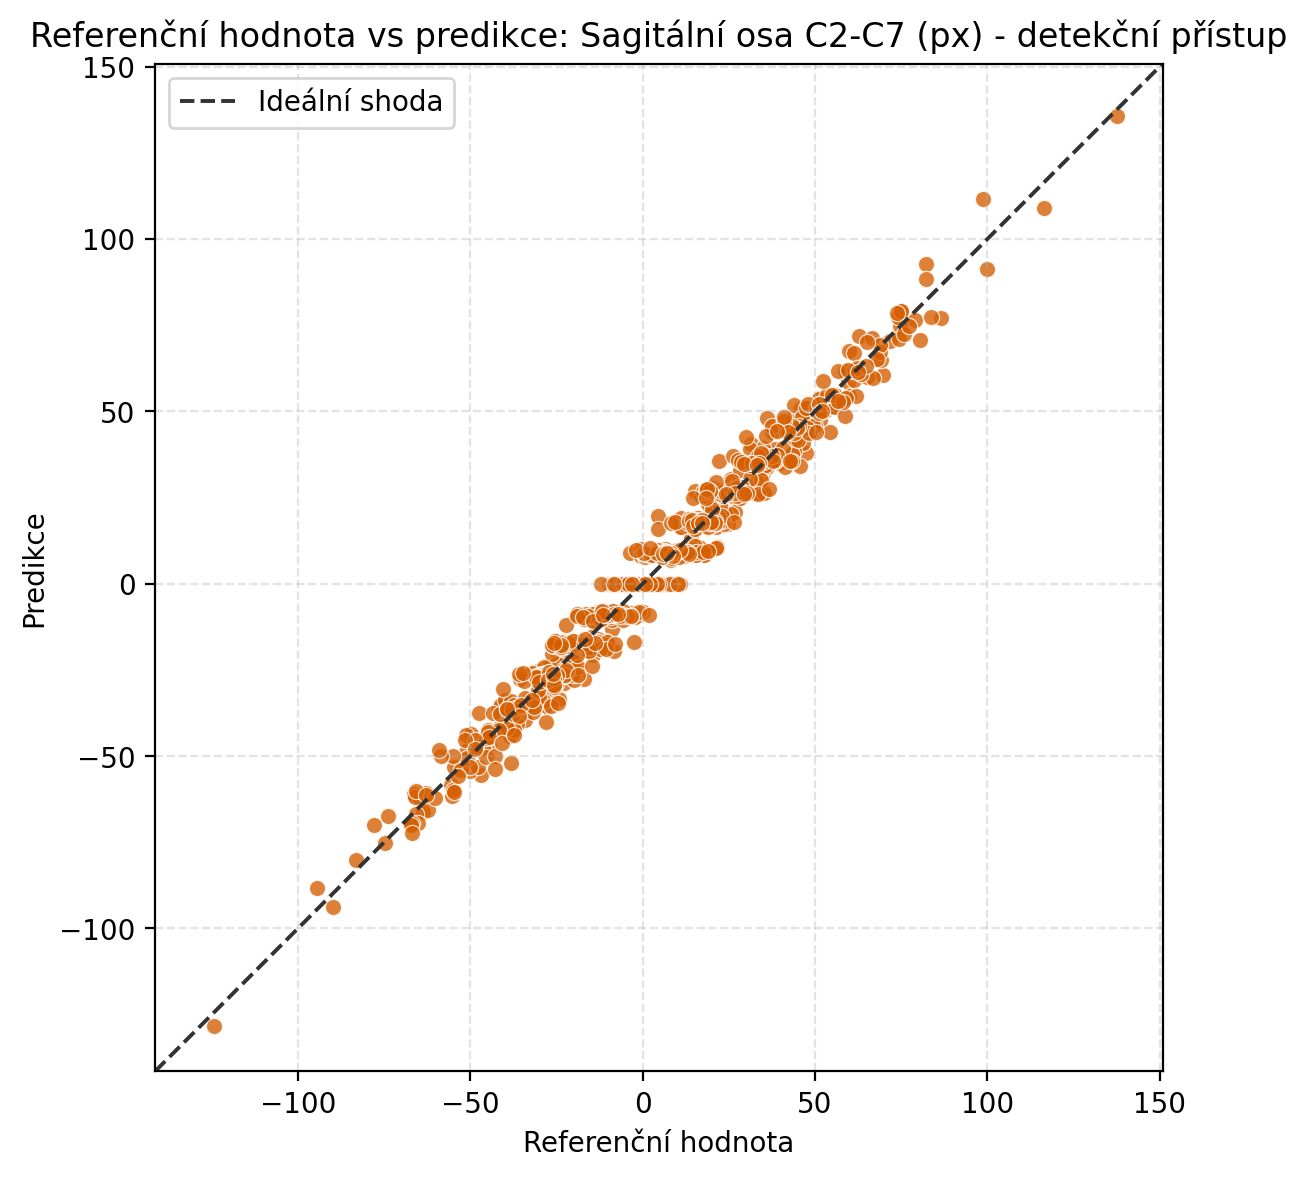
\includegraphics[width=0.75\linewidth]{images/results/test/det/scatter/SVA_C2_C7_px_scatter_gt_vs_pred.png}
    \caption{Porovnání referenčních a predikovaných hodnot sagitální vertikální osy C2--C7 u detekčního přístupu na testovací množině. Přerušovaná přímka znázorňuje ideální shodu predikce s referencí.}
    \label{fig:scatter_det_test_sva_c2_c7}
\end{figure}

\subsection{Sklon C2}

U metriky sklonu C2 dosáhl segmentační přístup na testovací části MAE 1{,}695$^\circ$ a RMSE 2{,}564$^\circ$, zatímco keypoint detection dosáhla MAE 4{,}963$^\circ$ a RMSE 6{,}278$^\circ$. Pearsonův korelační koeficient byl 0{,}958 pro segmentační model a 0{,}753 pro detekční přístup.

Rozdíl mezi oběma přístupy byl tedy výrazný nejen v úrovni absolutní chyby, ale také ve schopnosti zachovat vztah mezi referenčními a predikovanými hodnotami. Ve srovnání s trénovací částí se u segmentace zhoršila chyba z 1{,}334$^\circ$ na 1{,}695$^\circ$, zatímco u detekčního přístupu byla změna menší a hodnoty zůstaly velmi podobné.

\begin{figure}[H]
    \centering
    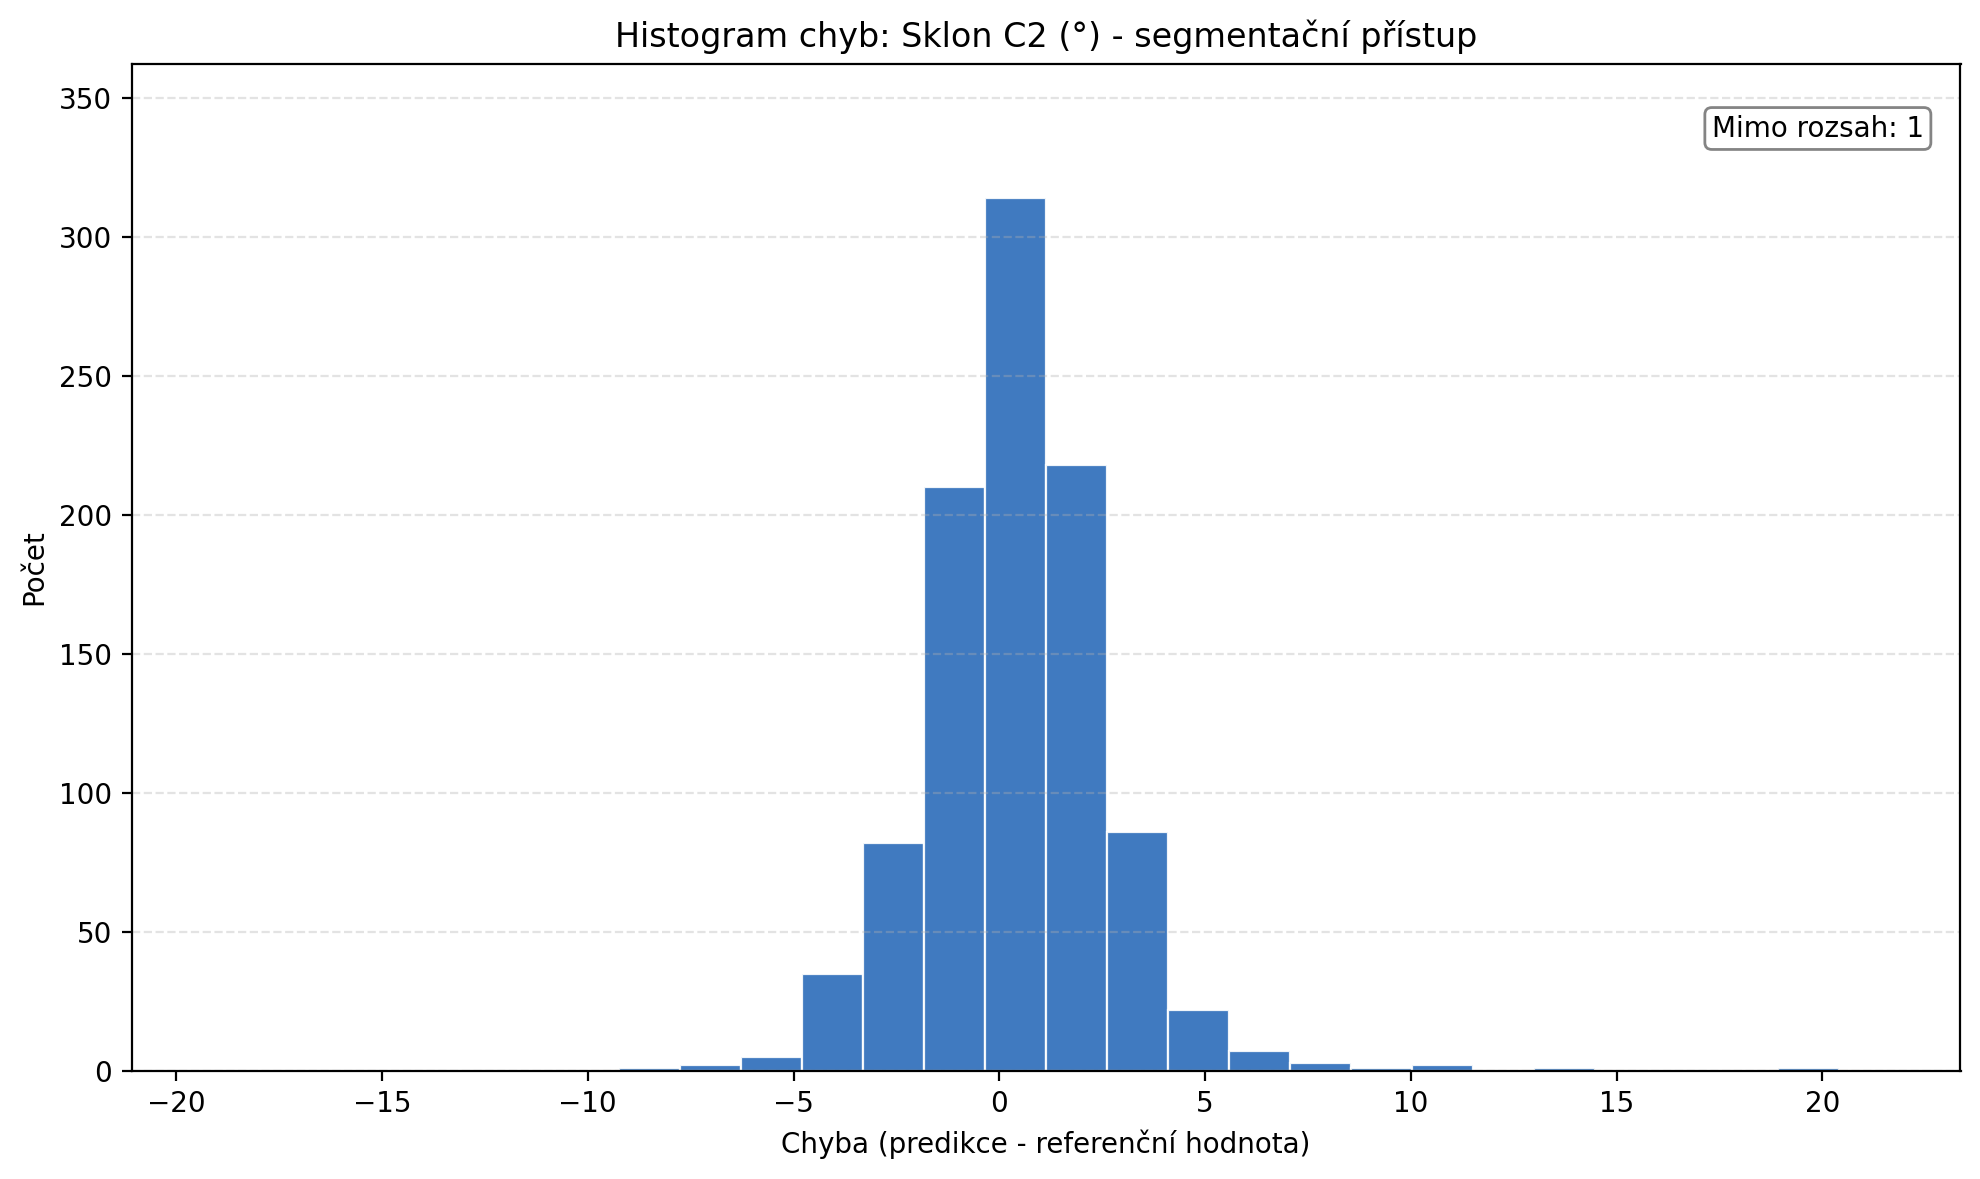
\includegraphics[width=0.75\linewidth]{images/results/test/seg/hist/Slope_C2_deg_error_histogram.png}
    \caption{Histogram chyb výpočtu sklonu obratle C2 u segmentačního přístupu na testovací množině. Chyba je definována jako rozdíl mezi predikovanou a referenční hodnotou.}
    \label{fig:hist_seg_test_slope_c2}
\end{figure}

\begin{figure}[H]
    \centering
    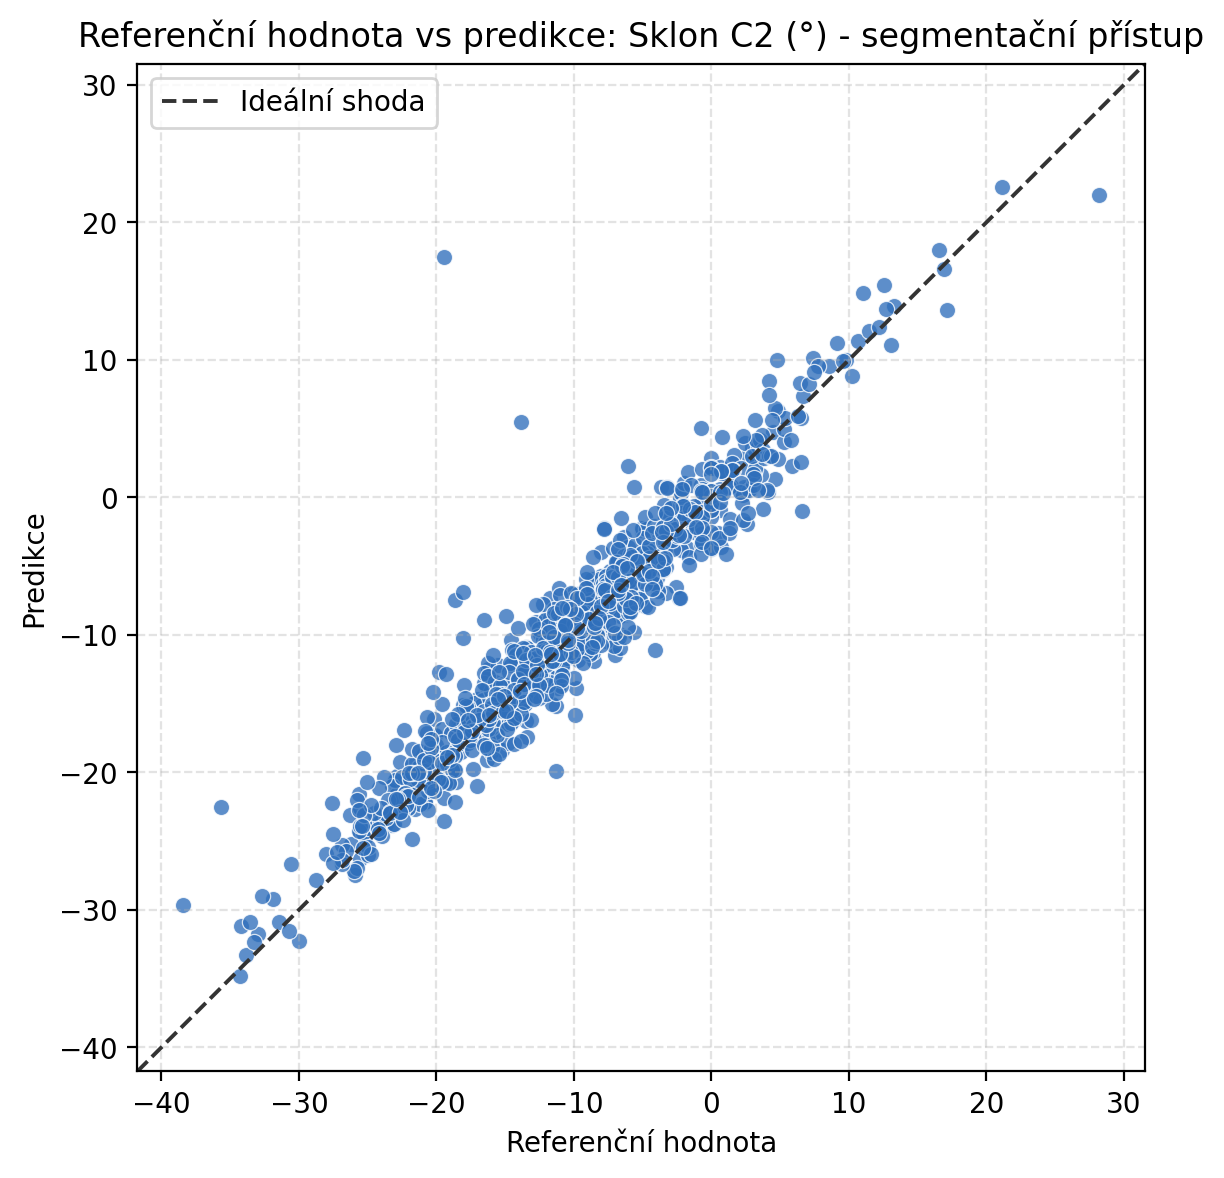
\includegraphics[width=0.75\linewidth]{images/results/test/seg/scatter/Slope_C2_deg_scatter_gt_vs_pred.png}
    \caption{Porovnání referenčních a predikovaných hodnot sklonu obratle C2 u segmentačního přístupu na testovací množině. Přerušovaná přímka znázorňuje ideální shodu predikce s referencí.}
    \label{fig:scatter_seg_test_slope_c2}
\end{figure}

\begin{figure}[H]
    \centering
    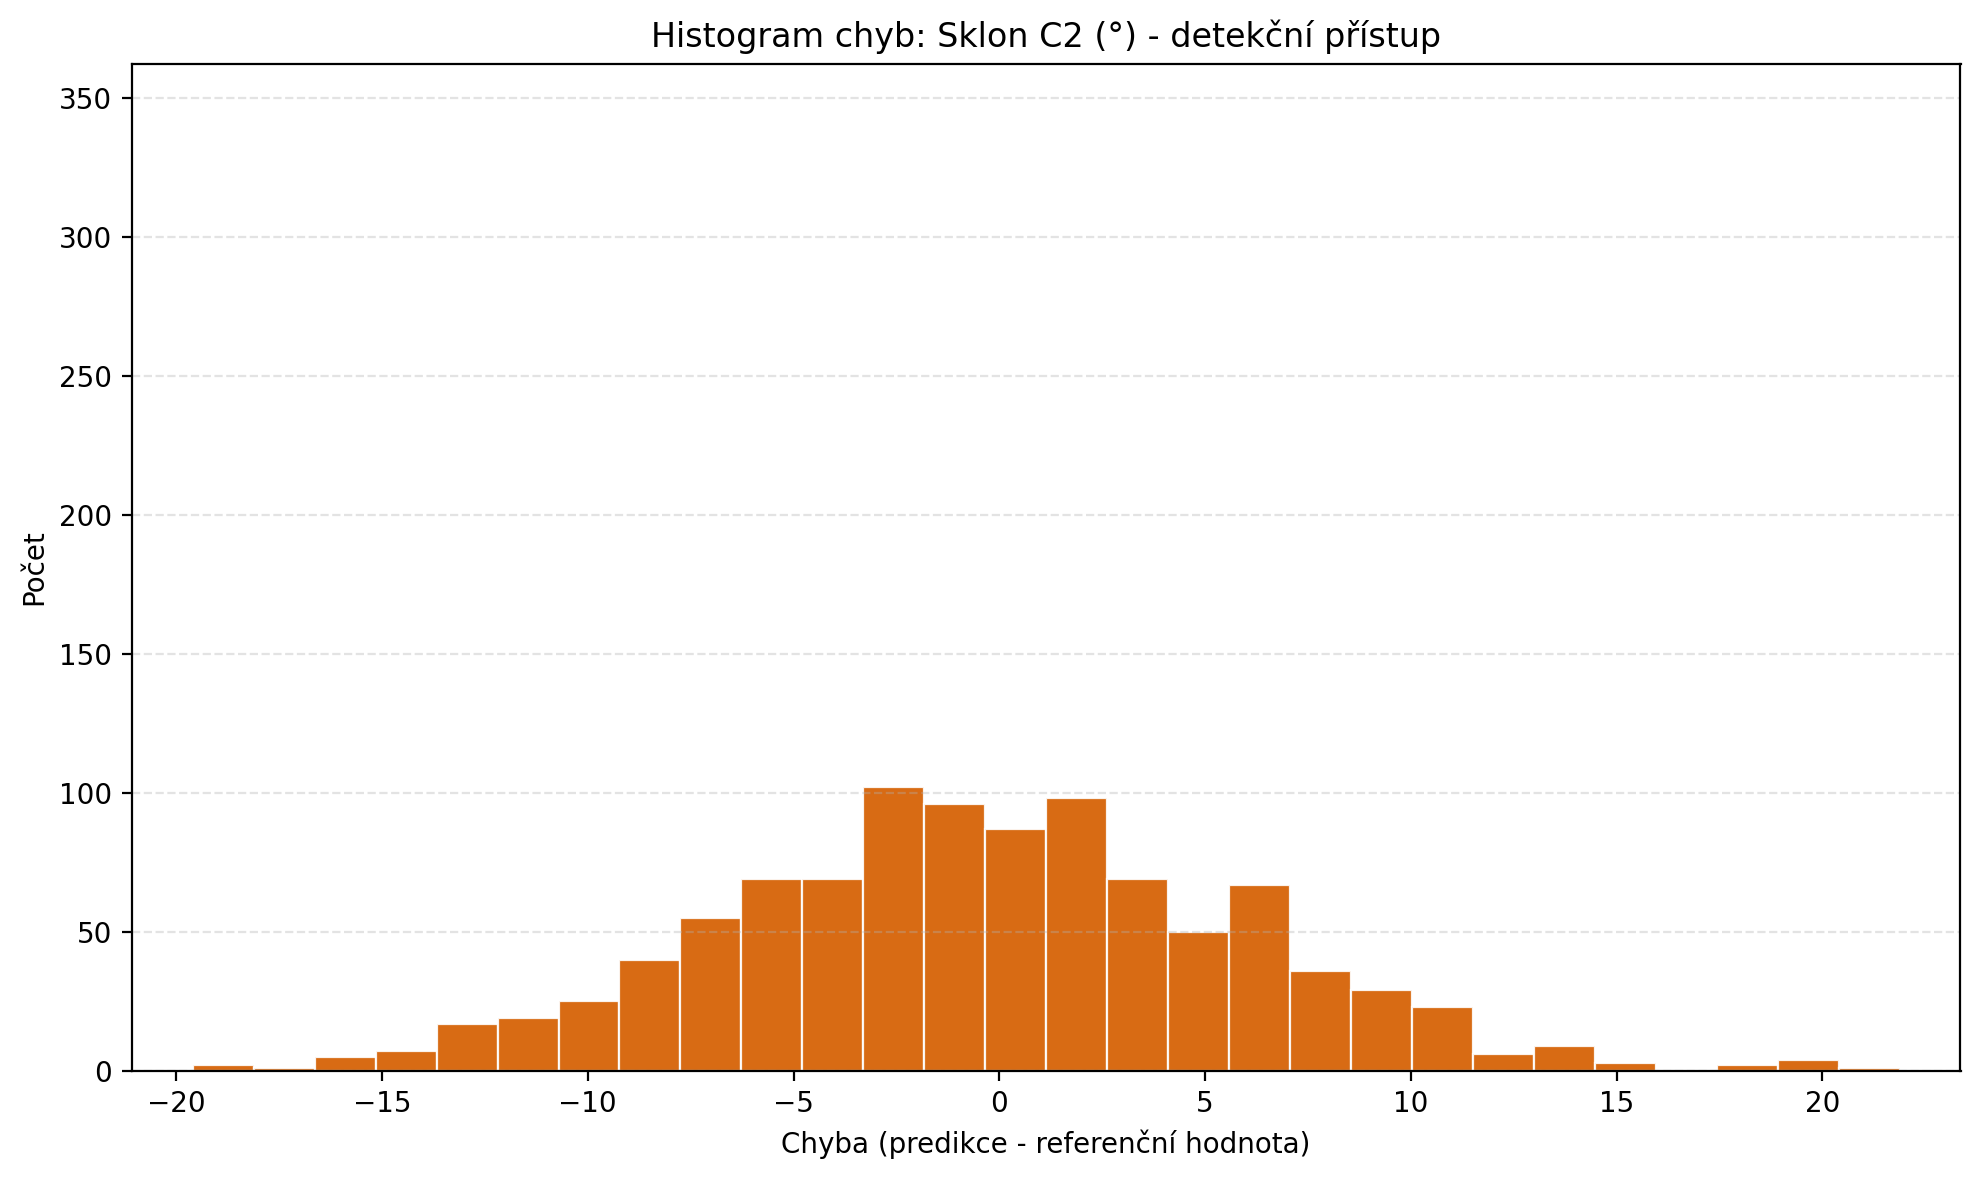
\includegraphics[width=0.75\linewidth]{images/results/test/det/hist/Slope_C2_deg_error_histogram.png}
    \caption{Histogram chyb výpočtu sklonu obratle C2 u detekčního přístupu na testovací množině. Chyba je definována jako rozdíl mezi predikovanou a referenční hodnotou.}
    \label{fig:hist_det_test_slope_c2}
\end{figure}

\begin{figure}[H]
    \centering
    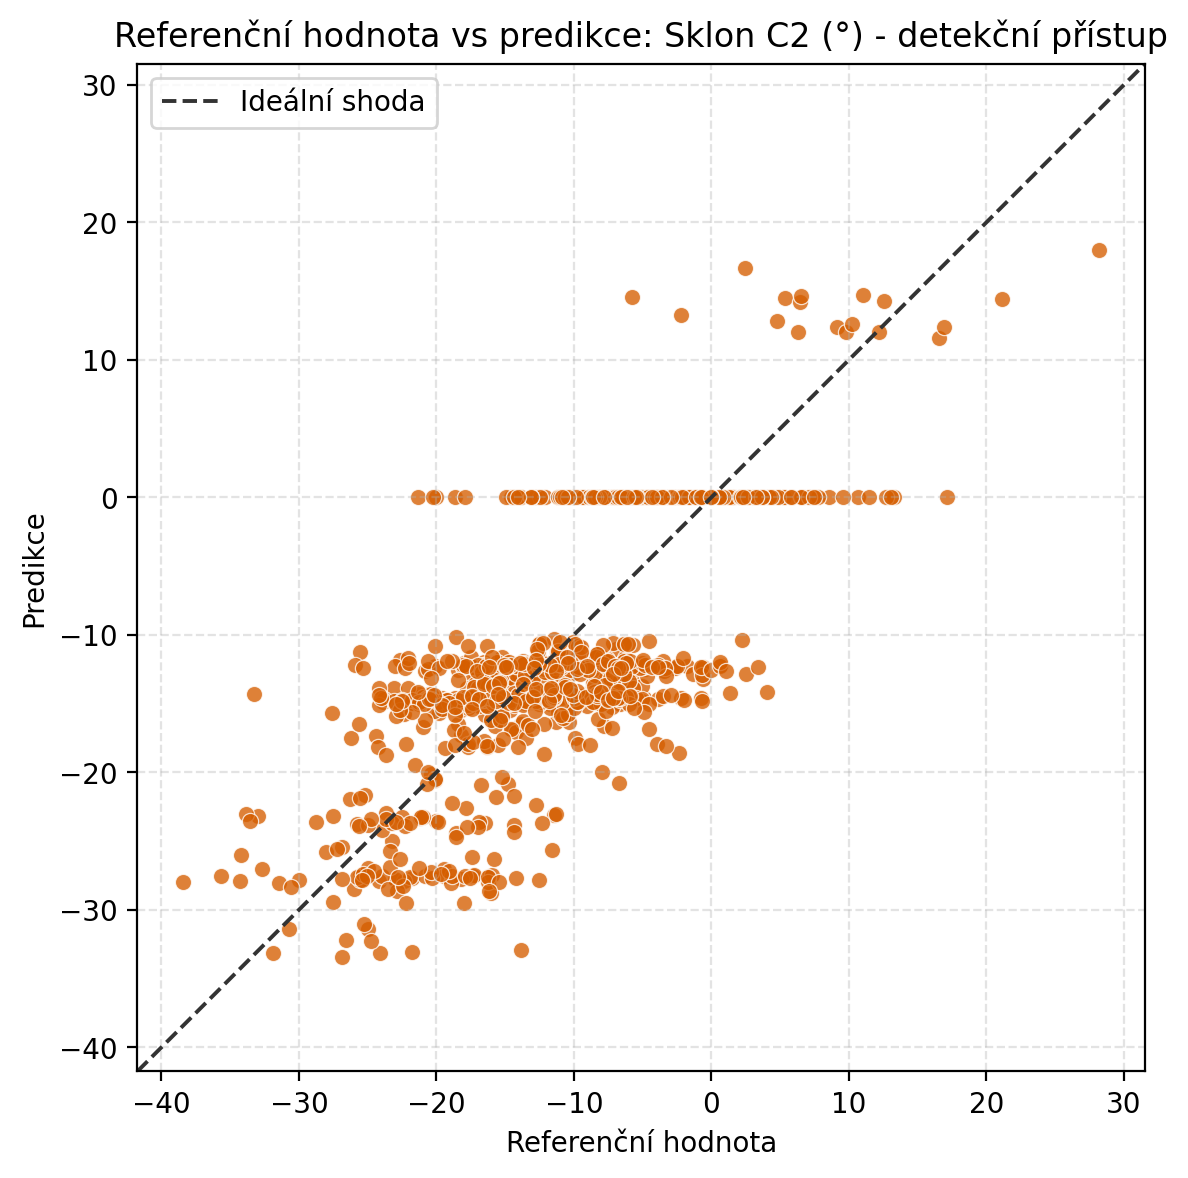
\includegraphics[width=0.75\linewidth]{images/results/test/det/scatter/Slope_C2_deg_scatter_gt_vs_pred.png}
    \caption{Porovnání referenčních a predikovaných hodnot sklonu obratle C2 u detekčního přístupu na testovací množině. Přerušovaná přímka znázorňuje ideální shodu predikce s referencí.}
    \label{fig:scatter_det_test_slope_c2}
\end{figure}

\subsection{Segmentové úhly}

U segmentových úhlů byl rozdíl mezi oběma přístupy nejvýraznější. Segmentační model dosahoval na testovací části napříč segmenty MAE přibližně 1{,}87$^\circ$ až 2{,}47$^\circ$, zatímco keypoint detection vykazovala MAE přibližně 6{,}13$^\circ$ až 6{,}40$^\circ$. Obdobný trend byl patrný i v hodnotách RMSE a Pearsonovy korelace.

Nejslabších výsledků dosáhly oba přístupy u segmentového úhlu C6--C7, přičemž segmentační model zde dosáhl korelace 0{,}600 a keypoint detection pouze 0{,}267. Naopak nejlepších výsledků ze segmentových úhlů bylo na testovací části dosaženo u segmentu C4--C5, kde segmentace dosáhla korelace 0{,}887. Ve srovnání s trénovací částí je u segmentových úhlů patrné zejména zhoršení segmentačního přístupu u segmentu C6--C7, kde korelace klesla z 0{,}829 na 0{,}600.


\section{Korelační analýza a analýza chyb}

Korelační matice absolutních chyb na testovací části ukazují, že segmentační přístup ve větší míře zachovával vzájemné vztahy mezi chybami jednotlivých klinických metrik než přístup založený na detekci klíčových bodů. Globální metriky zahrnuté do vyhodnocení, tedy Cobbův úhel C2--C7, sklon C2 a sagitální osa C2--C7, vykazovaly vyšší lineární shodu než segmentové úhly.

Z porovnání rozložení chyb je patrné, že u segmentačního modelu zůstávají absolutní chyby koncentrovány v užším okolí nižších hodnot, zatímco u keypoint detection jsou chyby rozprostřeny výrazně více. Tento trend se projevil zejména u Cobbova úhlu C2--C7 a u segmentových úhlů, kde detekční přístup vykazoval nejen vyšší MAE a RMSE, ale také nižší korelace.

\begin{figure}[H]
    \centering
    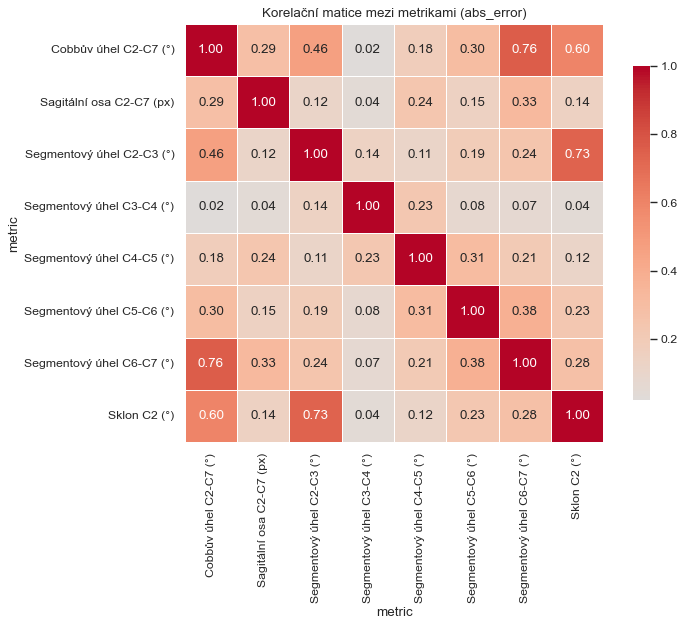
\includegraphics[width=0.95\linewidth]{images/results/test/seg/abs_error_correlation_matrix.png}
    \caption{Korelační matice absolutních chyb segmentačního modelu na testovací části sjednocené evaluační množiny.}
    \label{fig:corr_seg_test}
\end{figure}

\begin{figure}[H]
    \centering
    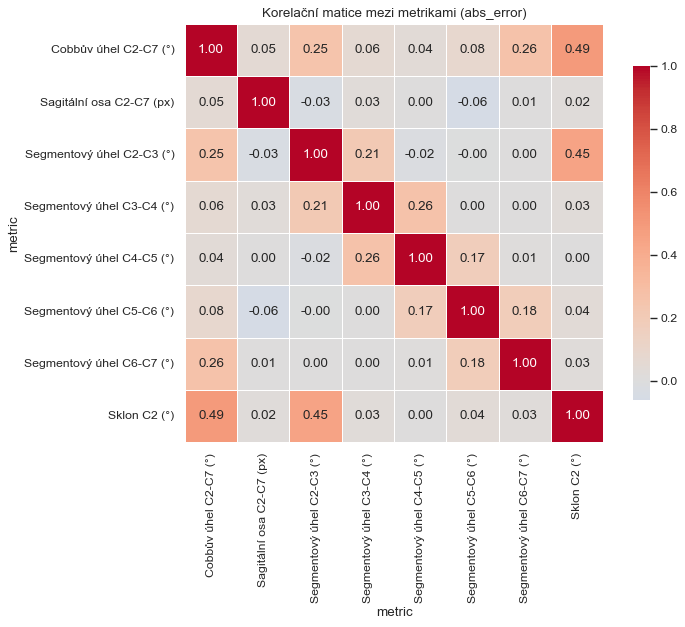
\includegraphics[width=0.95\linewidth]{images/results/test/det/abs_error_correlation_matrix.png}
    \caption{Korelační matice absolutních chyb detekčního modelu na testovací části sjednocené evaluační množiny.}
    \label{fig:corr_det_test}
\end{figure}

U segmentačního přístupu je patrná výraznější provázanost některých chyb. Nejsilnější vztah byl pozorován mezi chybou Cobbova úhlu C2--C7 a chybou segmentového úhlu C6--C7, dále mezi chybou sklonu C2 a segmentového úhlu C2--C3. To je očekávatelné, protože tyto metriky jsou geometricky závislé na podobných anatomických bodech nebo na krajních částech krční páteře. Pokud tedy dojde k nepřesné lokalizaci některých obratlů, chyba se může promítnout do více odvozených metrik současně.

U detekčního přístupu jsou korelace absolutních chyb obecně slabší a matice je méně strukturovaná. Výraznější vztah zůstává především mezi Cobbovým úhlem C2--C7 a sklonem C2 a mezi sklonem C2 a segmentovým úhlem C2--C3. To naznačuje, že chyby detekčního modelu jsou více rozptýlené mezi jednotlivé metriky a méně systematicky provázané než u segmentačního přístupu.

\section{Bland--Altmanova analýza}

Pro posouzení shody mezi referenčními hodnotami a hodnotami určenými automatickými metodami byla využita Bland-Altmanova analýza. Tato metoda byla navržena pro porovnávání dvou metod klinického měření a na rozdíl od korelačního koeficientu nehodnotí pouze sílu lineární závislosti, ale přímo rozdíly mezi oběma měřeními \cite{BlandAltman1986}. V grafu se pro každý snímek zobrazuje rozdíl mezi automaticky a referenčně určenou hodnotou proti jejich průměru. Díky tomu lze posoudit systematické vychýlení metody, rozptyl chyb, přítomnost odlehlých hodnot a případnou závislost chyby na velikosti měřené hodnoty.

V této práci je Bland-Altmanova analýza vhodná zejména proto, že cílem není pouze zjistit, zda automaticky vypočtené klinické metriky korelují s referenčními hodnotami, ale zda jsou s nimi dostatečně v souladu pro praktické použití. U metrik, jako je Cobbův úhel, segmentové úhly nebo sagitální vertikální osa, je důležité sledovat nejen průměrnou velikost chyby, ale také to, zda metoda hodnoty systematicky nadhodnocuje či podhodnocuje a zda se chyba nezvětšuje u vyšších nebo nižších hodnot dané metriky.

Pro každý vzorek se nejprve vypočítá rozdíl mezi predikcí a referenční hodnotou:
\[
d_i = \hat{y}_i - y_i,
\]
a průměr obou hodnot:
\[
m_i = \frac{\hat{y}_i + y_i}{2}.
\]
V Bland--Altmanově grafu je na vodorovné ose zobrazen průměr $m_i$ a na svislé ose rozdíl $d_i$. Dále se počítá průměrný rozdíl, označovaný jako systematická odchylka neboli bias:
\[
\bar{d} = \frac{1}{n}\sum_{i=1}^{n} d_i,
\]
a směrodatná odchylka rozdílů $s_d$. Meze shody jsou následně definovány jako:
\[
\bar{d} \pm 1{,}96s_d.
\]
Tyto meze přibližně určují interval, ve kterém by mělo ležet 95~\% rozdílů mezi predikcí a referenční hodnotou.

\begin{table}[H]
\centering
\caption{Bland--Altmanova analýza pro segmentační přístup na testovací množině.}
\label{tab:ba_seg_test}
\begin{tabular}{lrrrr}
\toprule
\textbf{Metrika} & \textbf{Bias} & \textbf{SD rozdílů} & \textbf{Dolní mez shody} & \textbf{Horní mez shody} \\
\midrule
Cobbův úhel C2--C7 [$^\circ$] & -0{,}14 & 4{,}27 & -8{,}52 & 8{,}24 \\
SVA C2--C7 [px] & 0{,}12 & 3{,}20 & -6{,}14 & 6{,}39 \\
Segmentový úhel C2--C3 [$^\circ$] & -0{,}24 & 3{,}07 & -6{,}25 & 5{,}78 \\
Segmentový úhel C3--C4 [$^\circ$] & -0{,}05 & 2{,}46 & -4{,}87 & 4{,}77 \\
Segmentový úhel C4--C5 [$^\circ$] & -0{,}01 & 2{,}47 & -4{,}84 & 4{,}82 \\
Segmentový úhel C5--C6 [$^\circ$] & 0{,}14 & 2{,}51 & -4{,}78 & 5{,}07 \\
Segmentový úhel C6--C7 [$^\circ$] & 0{,}01 & 4{,}68 & -9{,}16 & 9{,}18 \\
Sklon C2 [$^\circ$] & 0{,}47 & 2{,}52 & -4{,}48 & 5{,}41 \\
\bottomrule
\end{tabular}
\end{table}

\begin{table}[H]
\centering
\caption{Bland--Altmanova analýza pro detekční přístup na testovací množině.}
\label{tab:ba_det_test}
\begin{tabular}{lrrrr}
\toprule
\textbf{Metrika} & \textbf{Bias} & \textbf{SD rozdílů} & \textbf{Dolní mez shody} & \textbf{Horní mez shody} \\
\midrule
Cobbův úhel C2--C7 [$^\circ$] & -0{,}14 & 8{,}79 & -17{,}36 & 17{,}08 \\
SVA C2--C7 [px] & 0{,}24 & 4{,}58 & -8{,}73 & 9{,}22 \\
Segmentový úhel C2--C3 [$^\circ$] & 0{,}18 & 7{,}88 & -15{,}27 & 15{,}63 \\
Segmentový úhel C3--C4 [$^\circ$] & -0{,}52 & 7{,}98 & -16{,}16 & 15{,}12 \\
Segmentový úhel C4--C5 [$^\circ$] & 0{,}82 & 7{,}94 & -14{,}74 & 16{,}38 \\
Segmentový úhel C5--C6 [$^\circ$] & 0{,}10 & 7{,}78 & -15{,}14 & 15{,}35 \\
Segmentový úhel C6--C7 [$^\circ$] & -0{,}72 & 7{,}89 & -16{,}18 & 14{,}74 \\
Sklon C2 [$^\circ$] & -0{,}37 & 6{,}27 & -12{,}66 & 11{,}92 \\
\bottomrule
\end{tabular}
\end{table}


Z Bland--Altmanovy analýzy po jednotlivých metrikách (tabulky \ref{tab:ba_seg_test} a \ref{tab:ba_det_test}) vyplývá, že oba přístupy mají u většiny metrik malý bias, tedy nevykazují výrazné systematické nadhodnocování ani podhodnocování. Rozdíl mezi přístupy je však patrný především v šířce mezí shody. Segmentační přístup dosahuje u většiny úhlových metrik užších mezí shody, typicky přibližně v rozsahu $\pm 5^\circ$, což ukazuje na stabilnější predikce jednotlivých měření. Nejlepší shoda je patrná u segmentových úhlů C3--C4, C4--C5 a C5--C6, kde jsou meze shody relativně úzké a bias je blízký nule. Naopak slabší výsledek je u Cobbova úhlu C2--C7 a zejména u segmentového úhlu C6--C7, kde jsou meze shody širší. To může souviset s obtížnější lokalizací dolních krčních obratlů a větší citlivostí výsledného úhlu na chybu v poloze klíčových bodů.

\begin{figure}[H]
    \centering
    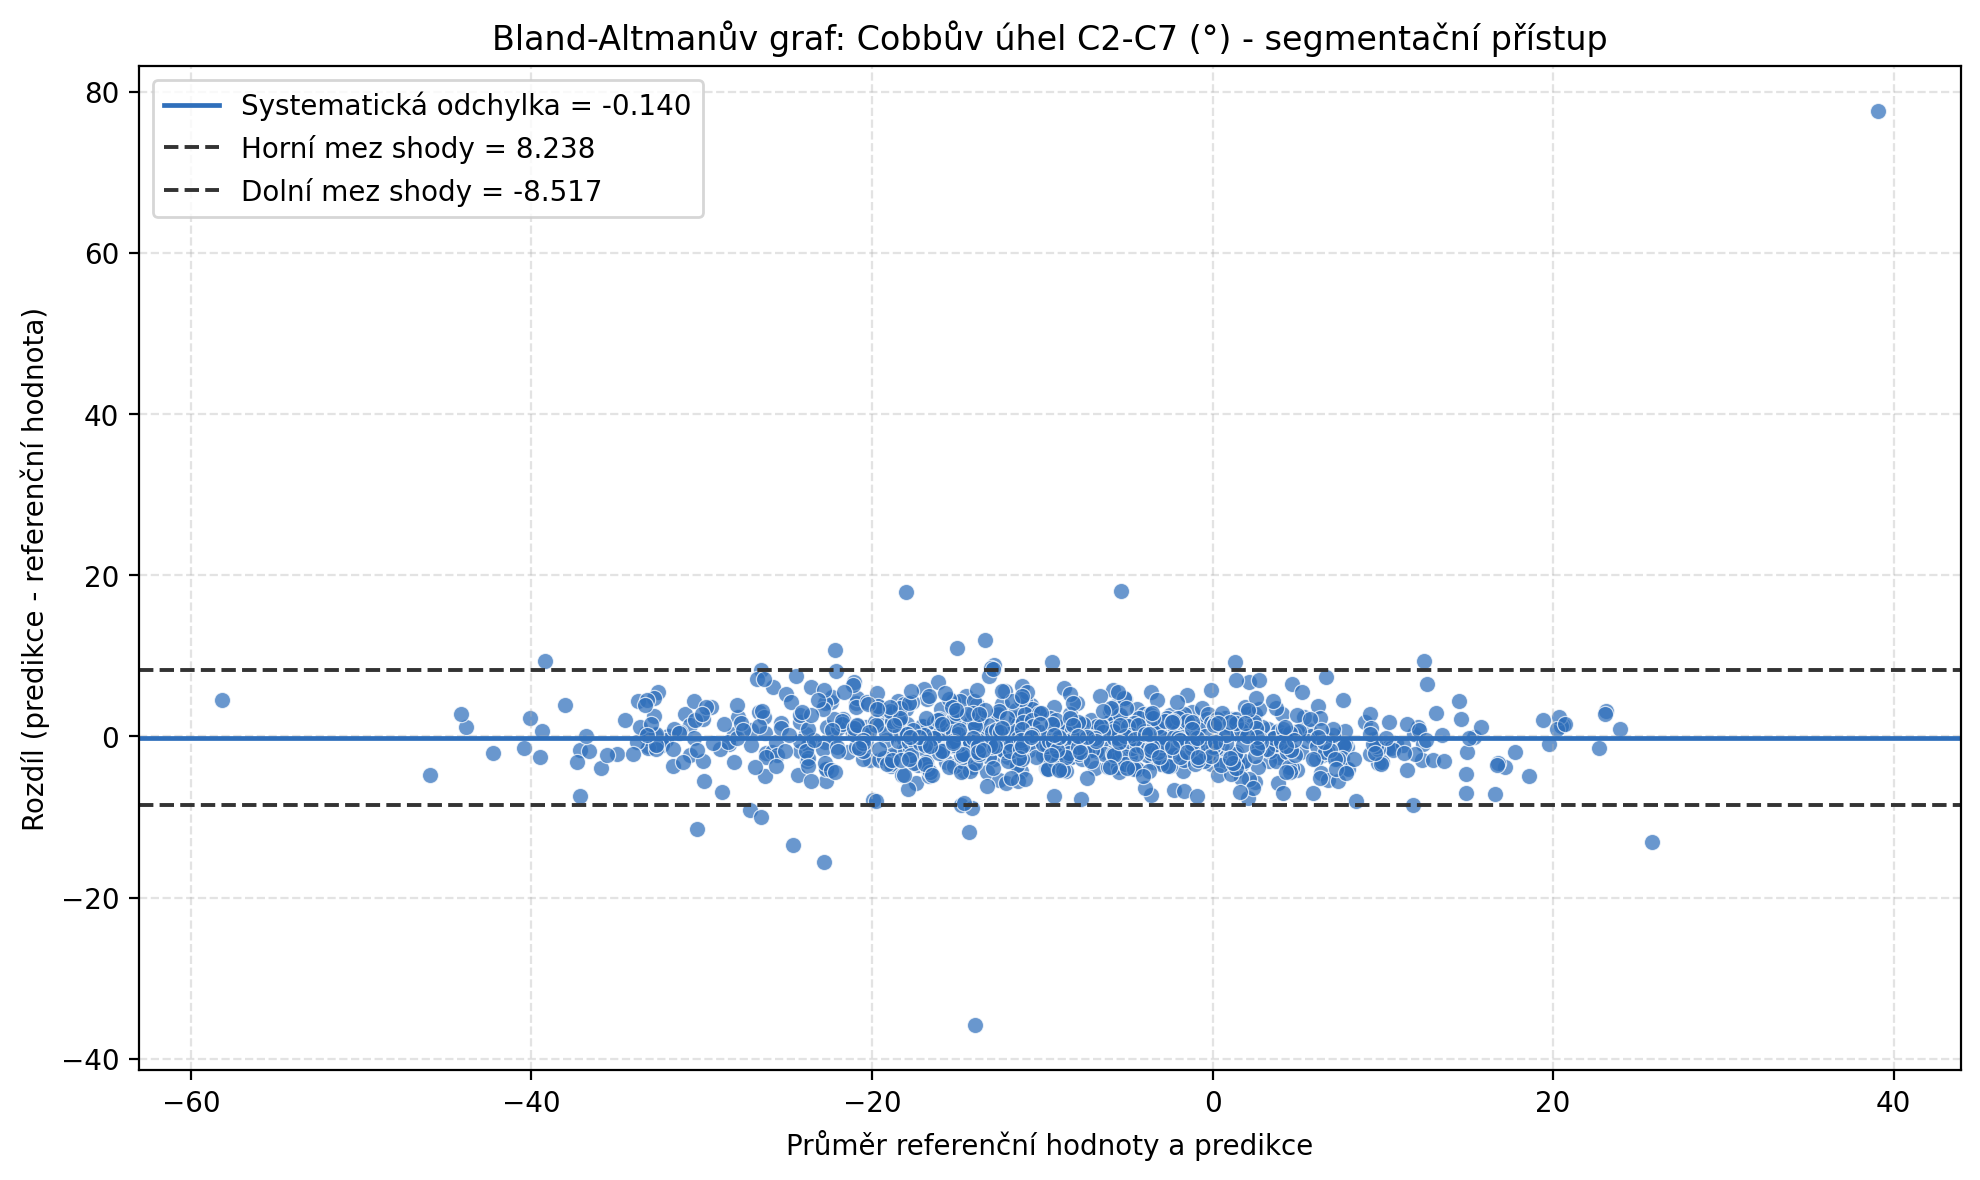
\includegraphics[width=0.95\linewidth]{images/results/test/seg/Cobb_C2_C7_deg_bland_altman.png}
    \caption{Bland--Altmanův graf pro Cobbův úhel C2--C7 u segmentačního přístupu na testovací množině.}
    \label{fig:bland_altman_seg}
\end{figure}

\begin{figure}[H]
    \centering
    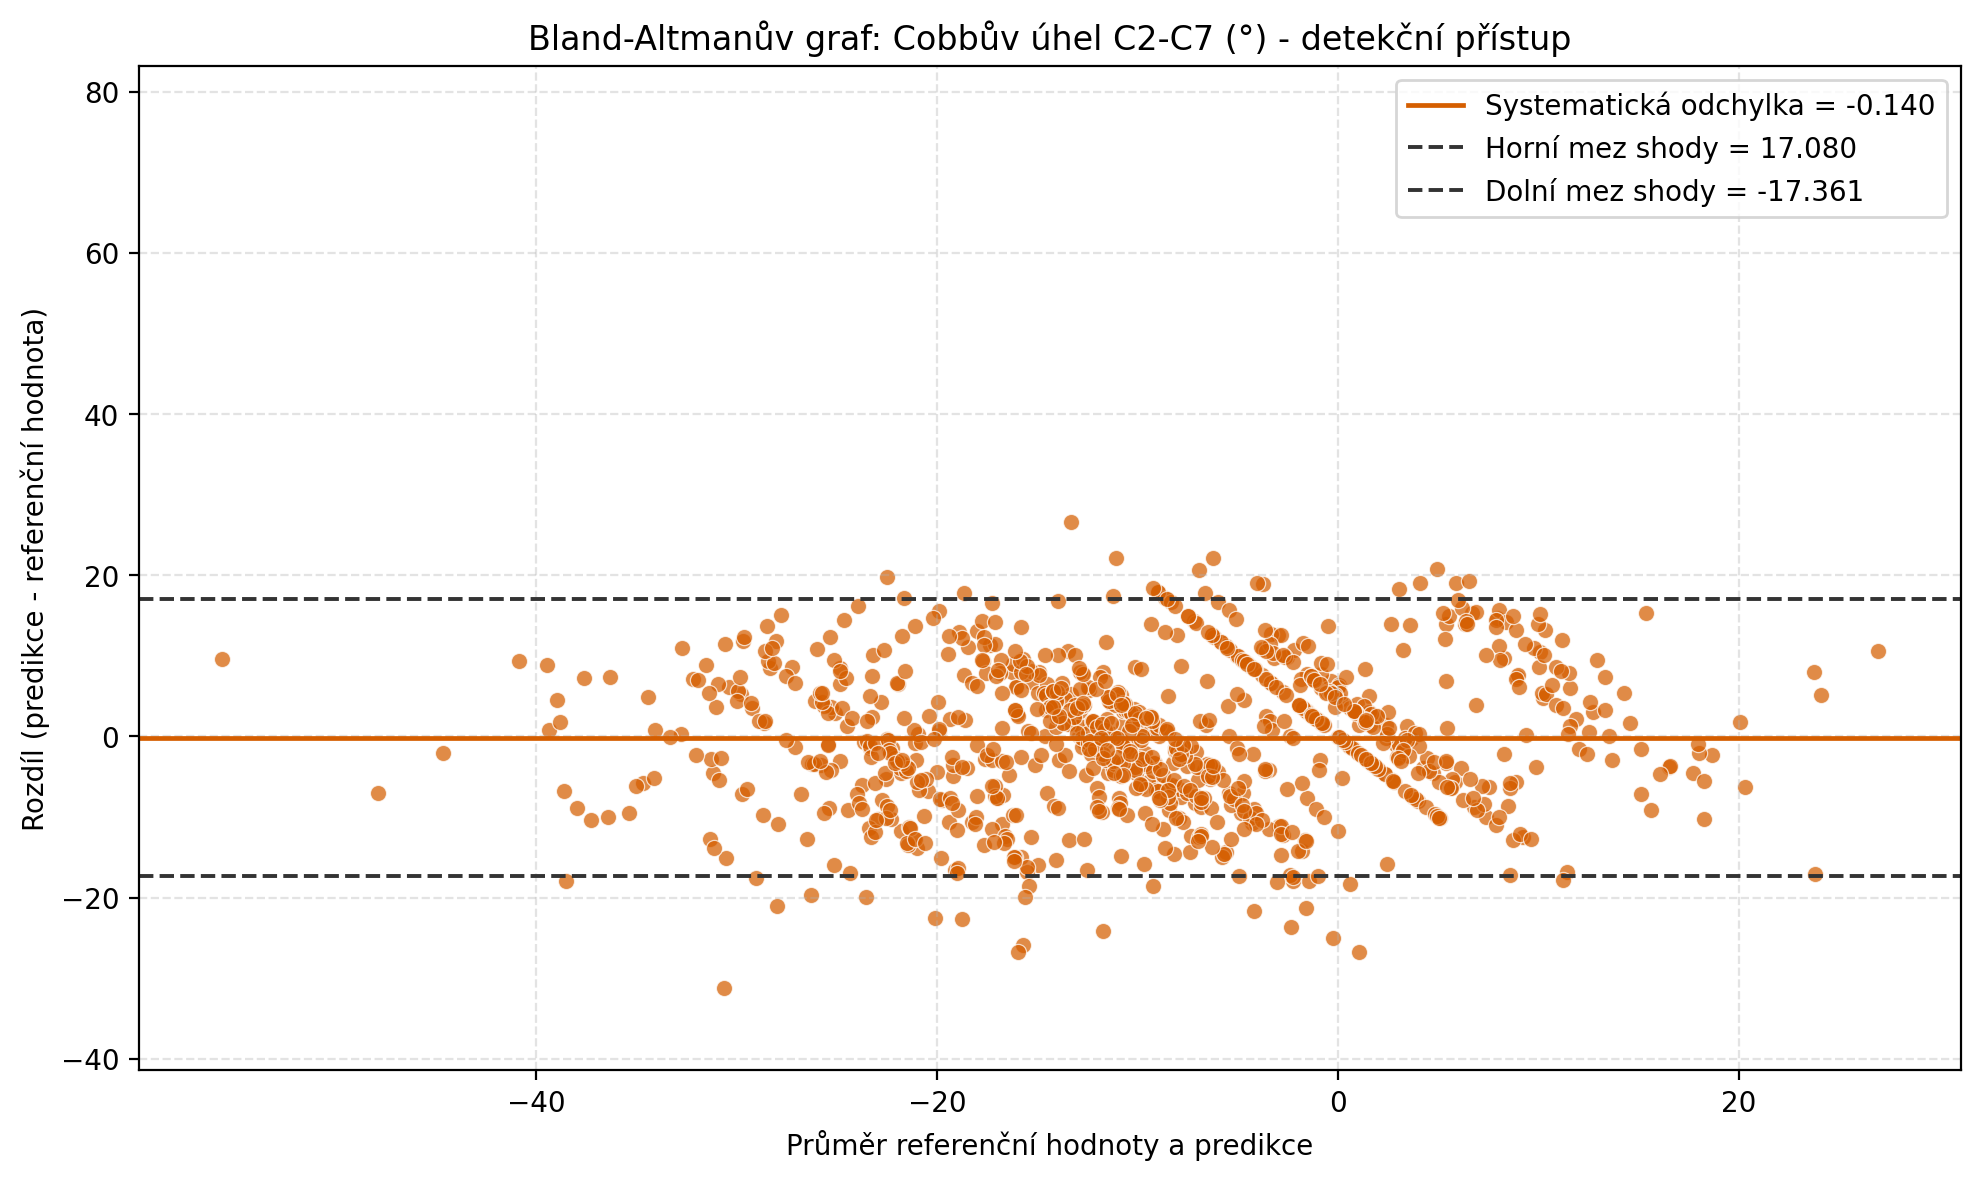
\includegraphics[width=0.95\linewidth]{images/results/test/det/Cobb_C2_C7_deg_bland_altman.png}
    \caption{Bland--Altmanův graf pro Cobbův úhel C2--C7 u přímé detekce klíčových bodů na testovací množině.}
    \label{fig:bland_altman_det}
\end{figure}


Detekční přístup má podobně nízký bias, avšak podstatně širší meze shody. U Cobbova úhlu C2--C7 dosahují meze shody přibližně $\pm 17^\circ$, což značí výrazně větší rozptyl chyb oproti segmentačnímu přístupu, kde se meze pohybují okolo $\pm 8^\circ$. Podobný trend je patrný také u segmentových úhlů, kde se meze shody pohybují přibližně v rozsahu $\pm 15^\circ$ (tento rozdíl je vidět na obrázcích \ref{fig:bland_altman_seg} a \ref{fig:bland_altman_det}). To znamená, že detekční model sice v průměru nemusí být výrazně vychýlený, ale jednotlivé predikce jsou méně stabilní. Výjimkou je metrika SVA C2--C7, kde jsou meze shody u detekčního přístupu stále relativně úzké v porovnání s ostatními metrikami, i když zůstávají širší než u segmentačního přístupu.

Celkově lze říci, že segmentační přístup dosahuje podle Bland--Altmanovy analýzy lepší shody s referenčními hodnotami. Rozhodující není pouze velikost biasu, který je u obou metod nízký, ale zejména šířka mezí shody. Užší meze shody u segmentačního přístupu ukazují, že tento model poskytuje konzistentnější výsledky a je vhodnější pro přesnější výpočet klinických metrik.


\section{Srovnání výpočetní náročnosti}

Výpočetní náročnost obou přístupů byla hodnocena na výpočetním uzlu GPU clusteru, jehož hardwarová a softwarová konfigurace je uvedena v tabulce~\ref{tab:runtime_hw_sw}. Měření bylo provedeno při dávce o velikosti jednoho snímku a bez započítání ukládání mezivýstupů na disk. Před vlastním měřením bylo provedeno 20 inicializačních průchodů, které nebyly zahrnuty do výsledného vyhodnocení. Samotné hodnocení bylo následně provedeno na 4\,943 snímcích. U keypoint detection bylo možné úspěšně vypočítat klinické metriky pro všechny vyhodnocené snímky. U segmentačního přístupu bylo úspěšně dokončeno 4\,935 z 4\,943 případů, přičemž v osmi případech nebylo možné dopočítat všechny metriky z důvodu chybějícího bodu \texttt{C7 bottom left}. Jednalo se tedy o stejné omezení, které se projevilo i v předchozí analýze přesnosti metrik.

\begin{table}[htbp]
\centering
\caption{Hardwarová a softwarová konfigurace výpočetního uzlu použitého pro měření výpočetní náročnosti.}
\label{tab:runtime_hw_sw}
\begin{tabular}{ll}
\hline
Parametr & Hodnota \\
\hline
GPU & NVIDIA L4 \\
Grafická paměť GPU & 23~GB \\
CPU & 2$\times$ AMD EPYC 7513 32-Core Processor \\
Počet fyzických jader CPU & 64 \\
Počet vláken CPU & 128 \\
Operační paměť & 125~GiB \\
Python & 3.10.4 \\
PyTorch & 2.4.1+cu121 \\
CUDA v PyTorch buildu & 12.1 \\
Verze ovladače NVIDIA & 565.57.01 \\
CUDA verze hlášená ovladačem & 12.7 \\
\hline
\end{tabular}
\end{table}

\subsection{Časová náročnost}

Časová náročnost byla hodnocena měřením doby preprocessingu, času vlastní inference modelu, času postprocessingu, času výpočtu klinických metrik a celkového end-to-end času zpracování jednoho snímku. Souhrnné výsledky jsou uvedeny v tabulce~\ref{tab:runtime_total}. Keypoint detection dosáhla průměrného celkového času 22{,}73~ms na snímek, zatímco segmentační přístup 221{,}63~ms na snímek. Z hlediska celkového end-to-end zpracování byl tedy segmentační přístup přibližně 9{,}8krát pomalejší. Při přepočtu na průchodnost odpovídaly tyto hodnoty přibližně 43{,}99 snímku za sekundu pro keypoint detection a 4{,}51 snímku za sekundu pro segmentační přístup.

\begin{table}[htbp]
\centering
\caption{Souhrnné srovnání celkového času zpracování jednoho snímku.}
\label{tab:runtime_total}
\begin{tabular}{lrrrrr}
\hline
Přístup & $n$ & \shortstack{Průměr\\{[ms]}} & \shortstack{Medián\\{[ms]}} & \shortstack{95. percentil\\{[ms]}} & Snímky/s \\
\hline
Keypoint detection & 4943 & 22.73 & 22.59 & 24.70 & 43.99 \\
Segmentace & 4943 & 221.63 & 219.59 & 251.36 & 4.51 \\
\hline
\end{tabular}
\end{table}

Podrobnější rozklad času na jednotlivé části pipeline je uveden v tabulce~\ref{tab:runtime_breakdown}. U keypoint detection byly preprocessing a vlastní inference modelu časově srovnatelné, oba kroky se pohybovaly okolo 11~ms na snímek. Postprocessing i samotný výpočet klinických metrik představovaly pouze malou část celkového času.

U segmentačního přístupu byla situace odlišná. Uváděný čas inference 8{,}27~ms odpovídá celému volání \texttt{sliding\_window\_inference} nad jedním snímkem, tedy všem výřezům potřebným pro zpracování daného obrazu, nikoli času jednoho jednotlivého okna. Rozhodující část časové náročnosti však tvořil postprocessing, který zahrnoval prahování masky, morfologické čištění, anatomické přeznačení segmentovaných oblastí a extrakci anatomických bodů. Tento krok dosáhl u segmentačního přístupu průměrné hodnoty 191{,}17~ms na snímek, zatímco u keypoint detection pouze 0{,}43~ms. Právě postprocessing tedy představoval hlavní příčinu vyšší celkové časové náročnosti segmentační metody.

\begin{table}[htbp]
\centering
\caption{Rozklad průměrného času zpracování jednoho snímku na jednotlivé části pipeline.}
\label{tab:runtime_breakdown}
\begin{tabular}{lrrrr}
\hline
Přístup & \shortstack{Preprocessing\\{[ms]}} & \shortstack{Inference\\{[ms]}} & \shortstack{Postprocessing\\{[ms]}} & \shortstack{Výpočet\\metrik {[ms]}} \\
\hline
Keypoint detection & 11.12 & 11.12 & 0.43 & 0.05 \\
Segmentace & 22.10 & 8.27 & 191.17 & 0.06 \\
\hline
\end{tabular}
\end{table}

Výsledky ukazují, že přístup založený na detekci klíčových bodů je z hlediska časové náročnosti výrazně rychlejší. Zároveň je však patrné, že rozdíl mezi metodami nevychází primárně z doby samotné inference neuronové sítě, ale především z odlišné náročnosti navazujícího postprocessingu.

\subsection{Paměťová náročnost}

Paměťová náročnost byla hodnocena na stejném výpočetním uzlu a stejné evaluační množině pomocí samostatného benchmarku. Ten sledoval využití pracovní paměti procesu a u CUDA zařízení také paměť GPU. Pro porovnání metod byl jako hlavní ukazatel zvolen špičkový nárůst alokované GPU paměti během zpracování jednoho snímku (vzorec \ref{eq:gpu_peak_memory_increase}). Tento údaj vyjadřuje, o kolik se zvýšila alokovaná paměť GPU oproti stavu před začátkem zpracování daného snímku.

\begin{equation}
\Delta M_{\mathrm{GPU}}^{\mathrm{peak}}
=
\max_{t \in T}
\left(
M_{\mathrm{GPU}}^{\mathrm{alloc}}(t)
\right)
-
M_{\mathrm{GPU}}^{\mathrm{alloc}}(t_0),
\label{eq:gpu_peak_memory_increase}
\end{equation}

kde $\Delta M_{\mathrm{GPU}}^{\mathrm{peak}}$ označuje špičkový nárůst alokované GPU paměti, $M_{\mathrm{GPU}}^{\mathrm{alloc}}(t)$ je alokovaná GPU paměť v čase $t$, $t_0$ je okamžik před začátkem zpracování snímku a $T$ představuje interval zpracování daného snímku.


Nejde tedy o celkovou obsazenou paměť GPU ani o velikost modelu, ale o dodatečnou paměť potřebnou pro samotnou inferenci jednoho snímku, tedy zejména pro vstupní tenzory, mezivýpočty a výstupy modelu. Tento ukazatel byl zvolen proto, že medián přírůstku pracovní paměti procesu byl u obou metod nulový a rezervovaná GPU paměť se v průběhu benchmarku prakticky neměnila.

Souhrnné výsledky jsou uvedeny v tabulce~\ref{tab:memory_total}. Keypoint detection dosáhla průměrného špičkového nárůstu alokované GPU paměti 21{,}72~MB na snímek, zatímco segmentační přístup 530{,}08~MB. Segmentační pipeline tedy vyžadovala přibližně 24{,}4krát vyšší špičkovou GPU paměť než přímá detekce klíčových bodů. Tento rozdíl je patrný i z mediánu a 95. percentilu, které u segmentačního přístupu dosáhly 535{,}05~MB a 546{,}29~MB, zatímco u keypoint detection pouze 21{,}08~MB a 25{,}11~MB.

\begin{table}[htbp]
\centering
\caption{Souhrnné srovnání špičkového nárůstu alokované GPU paměti při zpracování jednoho snímku.}
\label{tab:memory_total}
\begin{tabular}{lrrrr}
\hline
Přístup & $n$ & Průměr [MB] & Medián [MB] & 95. percentil [MB] \\
\hline
Keypoint detection & 4943 & 21.72 & 21.08 & 25.11 \\
Segmentace & 4943 & 530.08 & 535.05 & 546.29 \\
\hline
\end{tabular}
\end{table}

Podrobnější rozklad paměťové náročnosti na jednotlivé části pipeline je uveden v tabulce~\ref{tab:memory_breakdown}. U keypoint detection byla dominantním krokem inference modelu, která vyžadovala v průměru 20{,}70~MB špičkového nárůstu alokované GPU paměti. Preprocessing přidal pouze 0{,}75~MB a postprocessing ani výpočet klinických metrik již nevedly k měřitelnému navýšení GPU paměti.

U segmentačního přístupu byla rozhodující vlastní inference modelu, která dosáhla průměrného špičkového nárůstu 510{,}00~MB. Další navýšení paměťové náročnosti bylo spojeno s preprocessingem (4{,}84~MB) a zejména s postprocessingem (17{,}03~MB), který zahrnoval práci s více mezivýstupy segmentační masky a extrakci bodů. Z pohledu paměťové náročnosti je tedy segmentační metoda výrazně náročnější nejen časově, ale i paměťově, a to především kvůli inferenci modelu.

\begin{table}[htbp]
\centering
\caption{Rozklad průměrného špičkového nárůstu alokované GPU paměti na jednotlivé části pipeline.}
\label{tab:memory_breakdown}
\begin{tabular}{lrrrr}
\hline
Přístup & \shortstack{Preprocessing\\{[MB]}} & \shortstack{Inference\\{[MB]}} & \shortstack{Postprocessing\\{[MB]}} & \shortstack{Výpočet\\metrik {[MB]}} \\
\hline
Keypoint detection & 0.75 & 20.70 & 0.00 & 0.00 \\
Segmentace & 4.84 & 510.00 & 17.03 & 0.00 \\
\hline
\end{tabular}
\end{table}

Z hlediska praktického nasazení tedy keypoint detection nabízí nejen výrazně kratší dobu zpracování, ale také podstatně nižší nároky na GPU paměť. Segmentační přístup naproti tomu zůstává výpočetně i paměťově náročnější.

\section{Shrnutí hlavních zjištění}

Hlavní srovnání na testovací části sjednocené evaluační množiny ukázalo, že segmentační model dosáhl lepších výsledků ve všech osmi sledovaných klinických metrikách. Nižší chyby byly dosaženy jak u globálních charakteristik, tedy Cobbova úhlu C2--C7, sklonu C2 a sagitální osy C2--C7, tak u všech segmentových úhlů. Celkově se ukázalo, že rozdíly mezi segmentačním a detekčním přístupem se neprojevují pouze na úrovni lokalizace bodů, ale i na úrovni klinicky interpretovatelných metrik, které tvoří hlavní výstup této práce.

Zároveň se ukázalo, že segmentační přístup na testovacích datech mírně ztrácí oproti trénovací části, avšak i po tomto zhoršení zůstává výrazně přesnější než přímá detekce klíčových bodů. Detekční přístup si naproti tomu zachovává velmi podobné výsledky na trénovací i testovací části, ale jeho dosažená přesnost je ve všech sledovaných metrikách nižší.

Detekční přístup byl časově úspornější zejména díky jednodušší inferenční pipeline: po průchodu modelem stačí z jednotlivých heatmap určit polohu maxim a přepočítat souřadnice zpět do původního měřítka snímku. Segmentační přístup naproti tomu vyžaduje nejen samotnou predikci masek, ale také další kroky postprocessingu, například morfologické úpravy, analýzu souvislých komponent, extrakci kontur a odvození klíčových bodů. Z praktického hlediska tedy segmentační metoda představuje přesnější, ale výpočetně náročnější řešení z hlediska časové i paměťové náročnosti.

\chapter{Závěr}

Cílem této práce bylo navrhnout a ověřit postup pro automatickou analýzu RTG snímků krční páteře se zaměřením na segmentaci obratlů C2 až C7, extrakci anatomických klíčových bodů a následný výpočet vybraných radiologických metrik. Práce se soustředila na dvě odlišné formulace úlohy: na segmentační přístup, v němž jsou nejprve segmentovány jednotlivé obratle a teprve následně jsou ze segmentačních masek odvozeny klíčové body, a na přímou detekci klíčových bodů, kdy model predikuje body přímo ze vstupního snímku.

V rámci práce byla implementována a testována segmentační pipeline založená na architektuře U-Net. Součástí řešení bylo předzpracování dat, nastavení trénovací a validační pipeline, návrh postprocessingu segmentačních masek a vytvoření algoritmu pro extrakci 23 klíčových bodů odpovídajících anatomickým strukturám obratlů C2 až C7. Na základě těchto bodů lze dále stanovovat klinicky významné parametry, jako jsou Cobbův úhel C2--C7, sagitální vertikální osa nebo segmentové úhly. Důležitým přínosem práce je tedy nejen samotná segmentace obratlů, ale také převod obrazové informace na geometrickou reprezentaci přímo využitelnou pro další klinické hodnocení.

Současně byl do práce zahrnut i přístup založený na přímé detekci klíčových bodů, který představuje alternativu k segmentačnímu řešení. Porovnání obou přístupů ukazuje, že segmentační metoda poskytuje explicitní informaci o tvaru a rozsahu jednotlivých obratlů, zatímco přímá detekce klíčových bodů nabízí jednodušší inferenční pipeline z hlediska výpočetní náročnosti.

Za hlavní přínos práce lze považovat vytvoření uceleného zpracovatelského postupu, který propojuje segmentaci, postprocessing, extrakci klíčových bodů a přípravu podkladů pro výpočet radiologických metrik. Práce zároveň ukazuje, že metody hlubokého učení mají v oblasti automatické analýzy RTG snímků krční páteře značný potenciál, avšak jejich praktické nasazení je podmíněno dostatečnou kvalitou anotací, robustností vůči variabilitě vstupních snímků a pečlivou validací výsledků.

Možným směrem dalšího výzkumu je zejména rozšíření datasetu, důkladnější porovnání segmentačních a detekčních přístupů na větším souboru dat a případně také zlepšení extrakce klíčových bodů. Přínosné by bylo rovněž ověřit navržený postup na datech z jiných pracovišť a posoudit jeho generalizační schopnost v reálných klinických podmínkách.

\sloppy
\printbibliography[title=Seznam použitých zdrojů]

\appendix
\chapter{Externí přílohy\label{sec:ep}}

Externí přílohy této bakalářské práce jsou umístěny na adrese:\\ \url{https://github.com/JaroslavRadimsky/bp_ki_ujep}.

V~GitHub repozitáři se nachází tyto externí přílohy:

\begin{longtable}{ll}
	\hline
	bakalarska\_prace.pdf & text práce v~PDF \\
	bakalarska\_prace.tex & zdrojový kód práce v~\LaTeX{}u \\
	kitheses.cls & definice třídy dokumentů \\
	literature.bib & bibliografická databáze \\
	%zadani-bakalarske-prace.pdf & digitálně podepsané zadání bakalářské práce\\
	images & složka se všemi použitými i nepoužitými obrázky \\
	code & zdrojové kódy použité v~této práci \\
	\hline
\end{longtable}

Všechny tyto soubory jsou potřeba pro překlad dokumentu.

\end{document}
